\documentclass[11pt,letterpaper]{article}
\usepackage[utf8]{inputenc}
\usepackage[spanish]{babel}
\usepackage{graphicx}
\usepackage{subfigure}
\usepackage[top=1in, bottom=1in, right=1in, left=1in]{geometry}

%Paqueteria del glosario
\usepackage[hidelinks]{hyperref}
\usepackage[toc,style=altlistgroup,hyperfirst=false]{glossaries}
\makeindex
\makeglossaries

%%FORMATO PARA INGRESAR DEFINICION
%%%  \newglossaryentry{nombre} %como será escrito en el texto
%%%   {
%%%	   name={Nombre}, %como será escrito en el %%%   glosario
%%%	   description={aquí defines que es nombre}
%%%   }

\newglossaryentry{IPS}
{
	name={In-Plane Switching},
	description={Es un panel LCD clásico que tiene una disposición interna de los cristales líquidos que evita las fugas y pérdidas de luz, fenómeno que degradaría la calidad de imagen y la definición de colores, especialmente los oscuros. Cabe destacar que los colores dispuestos en dicho cristal líquido son iluminados por detrás con una segunda capa de focos LED.}
}

\newglossaryentry{CC BY-NC-SA}
{
	name={Atribución-NoComercial-CompartirIgual },
	description={Esta licencia permite a otros distribuir, remezclar, retocar, y crear a partir de tu obra de modo no comercial, siempre y cuando te den crédito y licencien sus nuevas creaciones bajo las mismas condiciones.}
}

\newglossaryentry{NPC}
{
	name={Non-playable character},
	description={Personaje no jugable en un juego.}
}

\newglossaryentry{Checkpoint}
{
	name={Punto de control},
	description={Punto de progreso temporal en el que el juego guardará esa posición y funcionara como punto de inicio mientras estés jugando.}
}

\newglossaryentry{Centla}
{
	name={Centla},
	description={Centla es un municipio del estado mexicano de Tabasco, localizado en la región del río Usumacinta y en la subregión de los Pantanos.}
}



\begin{document}
	\author{Hernández Bautista Yasmine Pilar, Márquez 		Hernández Karla Rocío}
	\title{Documento de diseño}
	\maketitle
	\tableofcontents
	
	\section{Concepto}
		\subsection{Título:} Yolotl.
		\subsection{Diseñadoras:} Hernández Bautista 				Yasmine Pilar, Márquez Hernández Karla Rocío.
    	\subsection{Género:} Plataforma. Aventura.
   		\subsection{Plataforma:} Dispositivos móviles Android. 
   		Dispositivo de prueba 1:
   		\begin{itemize}
   			\item Versión 7.0
   			\item Modelo ASUS X008DC
   			\item CPU MediaTek Quad Core Processor
   			\item GPU Mali T720
   			\item RAM 3GB LPDDR3
   			\item PANEL 5.2-inch
   			HD(1280 x 720) IPS display 
   			75 por ciento screen-to-body ratio
   			400nits brightness 
   		\end{itemize}
   		
   		Dispositivo de prueba 2:
   		\begin{itemize}
   			\item Versión 5.2
   			\item Modelo Huawei TAG-L13
   			\item CPU MediaTek MT6753 1,50 GHz
   			\item IPS TFT 16M colors 720 x 1280 px (5,00) 294 ppi
   			\item RAM 2GB
   			
   		\end{itemize}
   		
    	\subsection{Versión:} V02.12/07/17
   		\subsection{Sinopsis de jugabilidad:} 
 Haciendo uso de la pantalla touch del teléfono móvil y de una interfaz gráfica, el jugador controlara a Malinalli, siendo ella el personaje jugable durante todo el juego, salvo en un nivel en donde tanto ella como Xólotl serán los personajes jugables.   El jugador hará que Malinalli pueda moverse de izquierda a derecha, realice un salto o un salto doble, ataque con tonalli o dialogue con otros personajes.
\\
\par
En total el jugador deberá de pasar 10 niveles para terminar el juego. Cada nivel está diseñado para que el jugador tenga que superar diferentes plataformas y derrotar enemigos (enemigos comunes y jefes de nivel). Algunos niveles están más orientados a la superación de obstáculos, otros a la exploración y algunos al combate, siendo la constante entre todos (salvo el nivel introductorio), el tener que derrotar a un jefe al final del nivel.
\\
\par
La GUI contendrá cuatro botones(ver  figura): uno para moverse a la izquierda, otro para moverse a la derecha, otro más para saltar y uno para disparar tonalli. En la parte superior de la pantalla habrá dos iconos uno para indicar la cantidad de vida de Malinalli y otro para la cantidad de tonalli para disparar. La cantidad de tonalli disminuirá con cada ataque que el jugador efectué y cuando éste llegué a cero, el jugador podrá disparar hasta después de que se reestablezca la barra de tonalli o si logra obtener el ítem Flor de vainilla(ver figura \ref{fig:UsoTonalli} ). Cuando un disparo de tonalli colisiona con un enemigo, éste desaparece si es un enemigo común o se le infringe una cantidad de daño determinada en caso de que sea un jefe (Ver figura \ref{fig:InterEnemigo}). La vida de Malinalli disminuirá si recibe ataques de los enemigos o colisiona con alguno (ver figura \ref{fig:Danio}). Cada enemigo tiene una cantidad de daño asignada, siendo los jefes de cada nivel los enemigos con mayor capacidad de infringir daño. La partida acabará si la vida de Malinalli llega a cero. El jugador podrá recuperar vida con el ítem Grano de Cacao.

\begin{figure}
				\centering
				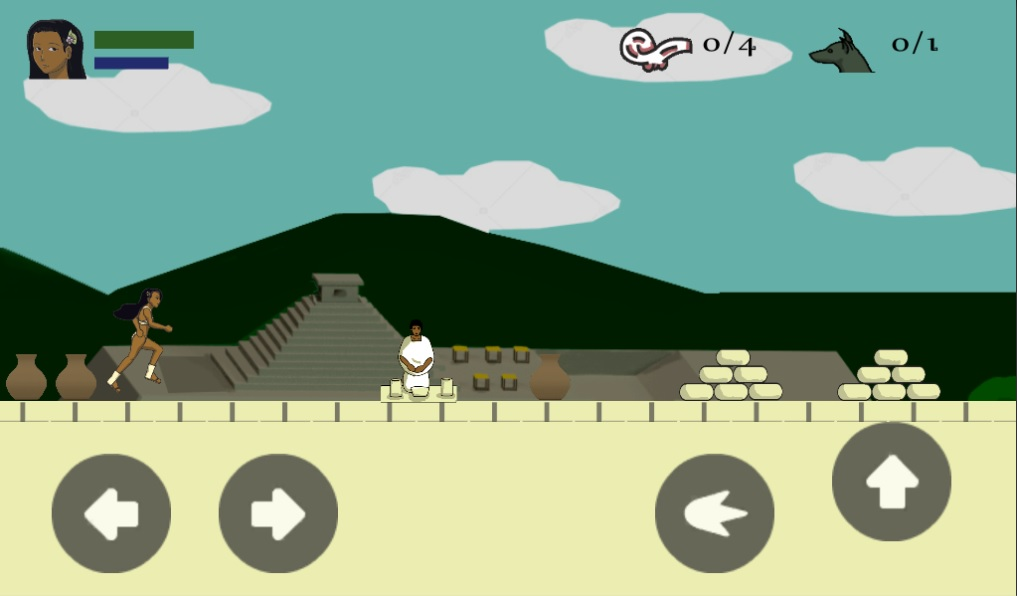
\includegraphics[height=0.3 \textheight]{Imagenes/ControlCorrerDer}
				\caption{1 Información del personaje jugable, barra verde indicador de la cantidad de vida, barra azul cantidad de tonalli. 2 Objetivos del nivel o información útil. 3 Botón moverse izquierda. 4 Botón moverse derecha. 5 Botón disparar tonalli. 6 Botón saltar.}
				\label{fig:GUI}
\end{figure}

\begin{figure}
				\centering
				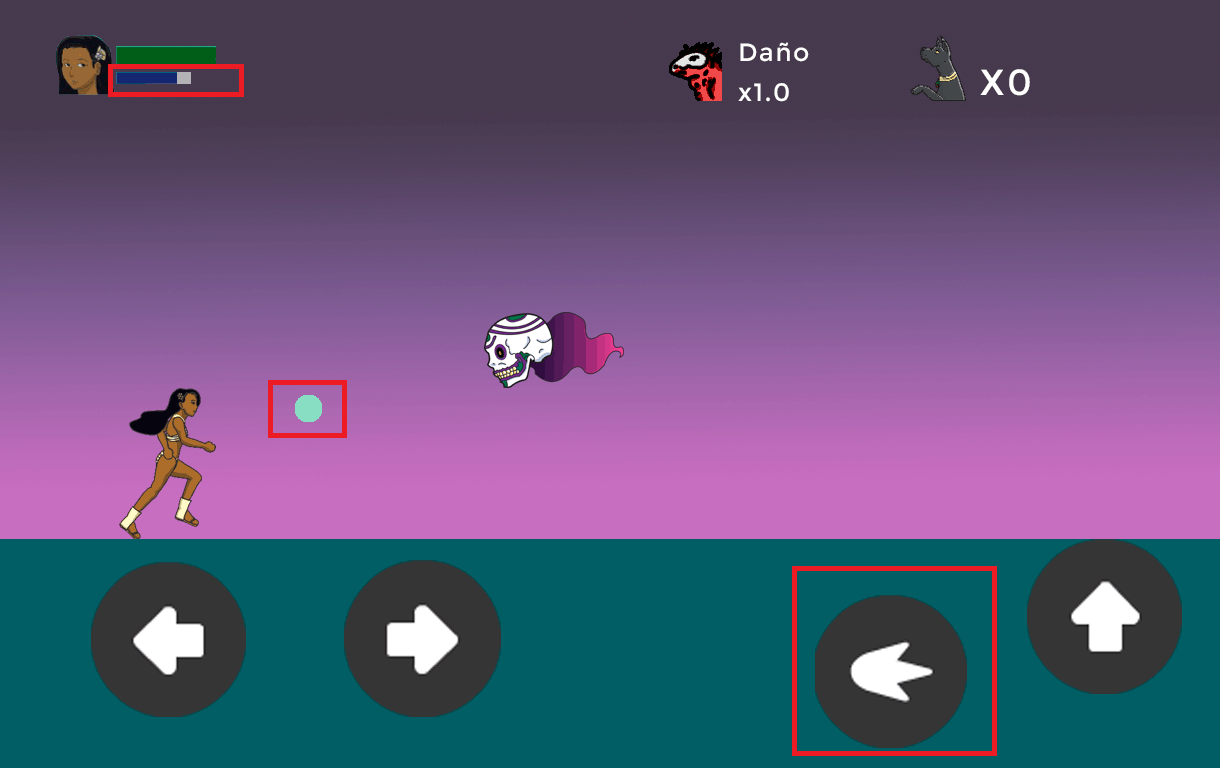
\includegraphics[height=0.3 \textheight]{Imagenes/nivel02_tonalli}
				\caption{Cuando el jugador dispara se consume una fracción de la barra de tonalli.}
				\label{fig:UsoTonalli}
\end{figure}

	\begin{figure}
  \centering
  \subfigure[Disparo de tonalli.]{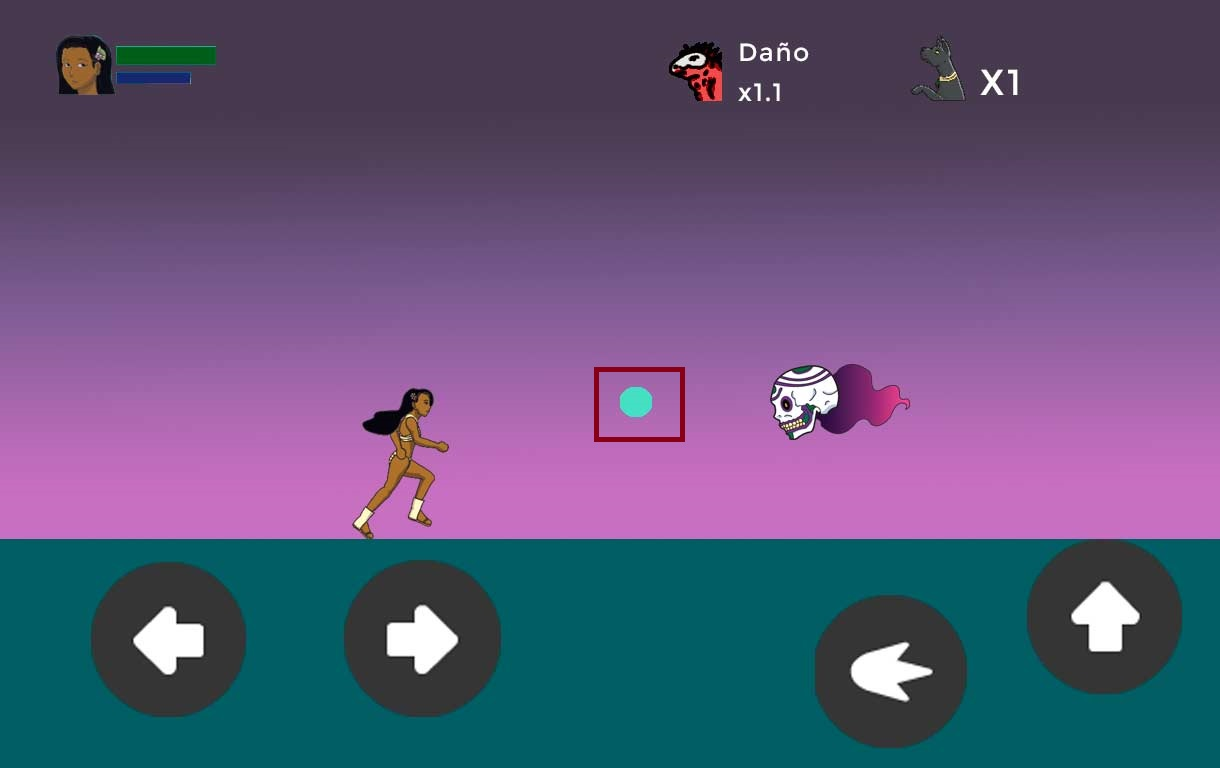
\includegraphics[width=0.45 \textwidth]{Imagenes/PantallaInteraccionEnemigo}}
   \subfigure[Colisión disparo de tonalli con enemigo común.]{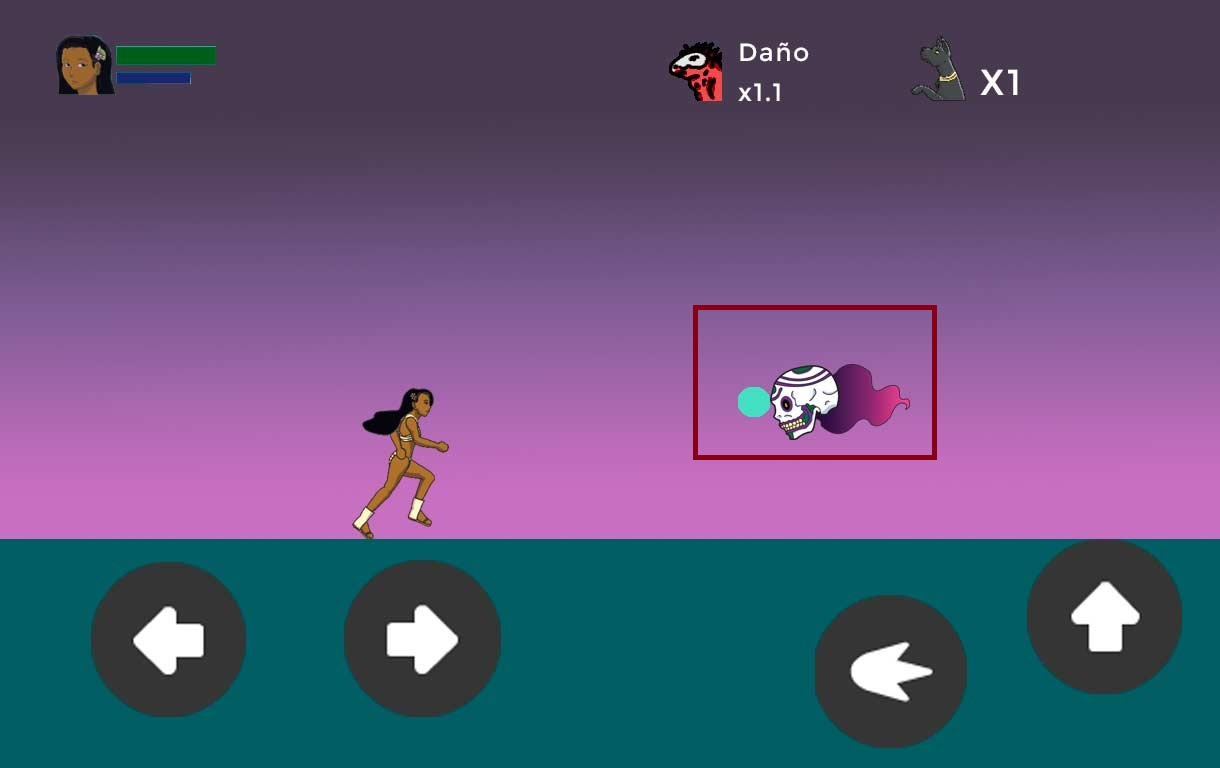
\includegraphics[width=0.45 \textwidth]{Imagenes/PantallaInteraccionEnemigo02}}
   \subfigure[Destrucción del enemigo y el disparo de tonalli.]{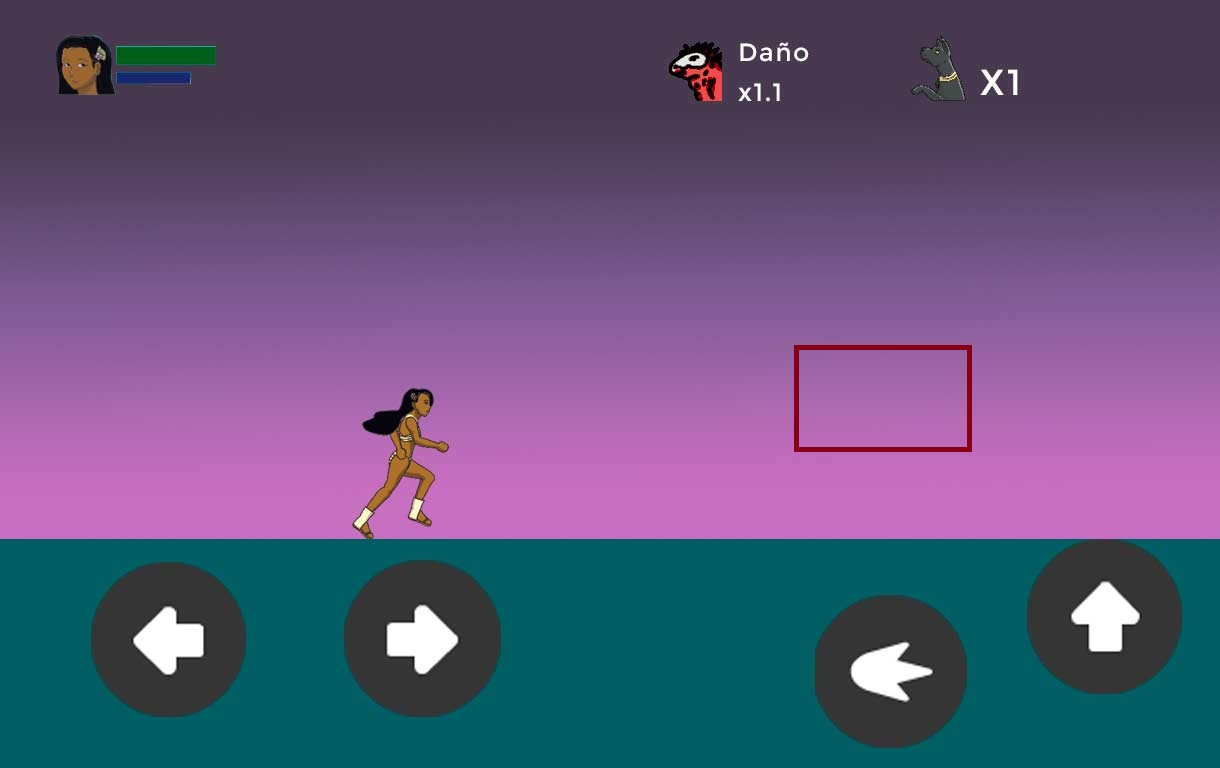
\includegraphics[width=0.45 \textwidth]{Imagenes/PantallaInteraccionEnemigo03}}
  \caption{Interacción entre el enemigo y el disparo de tonallia}
  \label{fig:InterEnemigo}
\end{figure} 

\begin{figure}
				\centering
				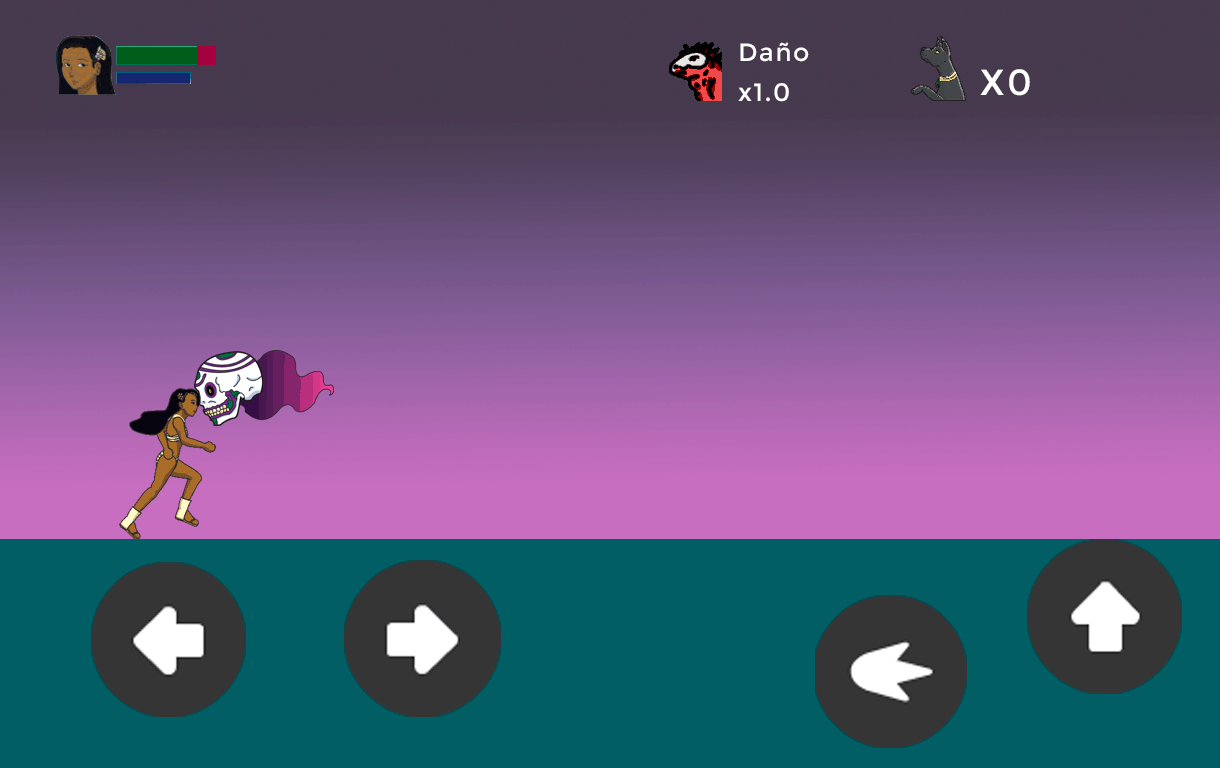
\includegraphics[height=0.3 \textheight]{Imagenes/nivel02_danio}
				\caption{Cuando el jugador colisiona con un enemigo el personaje jugable recibe daño y su cantidad de  vida disminuye, el daño recibido depende del enemigo.}
				\label{fig:Danio}
\end{figure}
  		
    	\subsection{Sinopsis de contenido:} 
La historia se centra en Malinalli Tenelpan, una joven esclava que desea revivir a su padre, y el dios Xólotl, un Dios exiliado que se ha ofrecido a revivir al padre de Malinalli a cambio de su ayuda, cuyo objetivo es restaurar el orden de la jerarquía divina luego de que Tezcatlipoca y Quetzalcóatl la sumergieran en un espiral de caos con sus múltiples batallas por el liderazgo de los dioses. 
\\
\par
Para cumplir sus objetivos, Malinalli y Xólotl bajaran al Mictlan. Ahí enfrentaran a los guardianes del Mictlan, que son Dioses de gran poder cuyas habilidades se relacionan con un aspecto de la muerte. Siendo el último a vencer el señor y gobernante del Mictlan: el dios Mictlantecuhtli.
\\
\par
A lo largo de la narrativa, el jugador irá descubriendo el pasado de los dos protagonistas, así como aprenderá sobre el funcionamiento del mundo de los dioses, sus reglas, su jerarquía y sus integrantes.

	\subsection{Categoría:}
A continuación se presentará una tabla comparativa que muestra la diferentes juegos que, por sus mecánicas o temática, pueden ser considerados como productos similares a Yolotl.
\begin{itemize}
	\item Guacamelee!!
	\begin{itemize}
		\item Microsoft Windows, OS X, Linux, PlayStation 3, PlayStation 4, PlayStation Vita, Wii U, Xbox 360, Xbox One.
		\item 103.12 a 206.03 (dependiendo de la plataforma)
		\item Plataforma, Metrodvania.
		\item Personas mayores de 10 años
		\item Diferencia: No es contexto de caracter histórico, no es móvil.
	\end{itemize}

\item Never Alone
\begin{itemize}
	\item Linux, Microsoft Windows, OS X, PlayStation 3, PlayStation 4, Wii U, Xbox One, iOS, Android.
	\item 150.00 a 89.00 (dependiendo de la plataforma)
	\item Plataforma, puzzle.
	\item Personas mayores de 10 años.
	\item Diferencia: No cuenta con estatus de vida o elementos de ataque del personaje, no es móvil.
\end{itemize}


\item Valiant Hearts
\begin{itemize}
	\item Microsoft Windows, Xbox One, PlayStation 4, PlayStation 3, wiistation 360, Android y iOS.
	\item 285.00
	\item Juego de Lógica. 
	\item Personas mayores de 13 años.
	\item Diferencia: No es un juego de plataforma, no es móvil.
\end{itemize}


\item Olympia rising.
\begin{itemize}
	\item Wii U.
	\item 95.11
	\item Acción y aventura.
	\item Mayores de 10 años.
	\item Diferencia: No es un juego móvil.
\end{itemize}


\item Jotun: Valhalla Edition.
\begin{itemize}
	\item PlayStation 4, Xbox One, Wii U, Microsoft Windows, GNU/Linux, Mac OS.
	\item 150.00
	\item Acción Aventura.
	\item Personas mayores de 13 años.
	\item Diferencia: No es un juego móvil, no es de plataforma.
\end{itemize}

\end{itemize}

	\subsection{Licencia:}
Atribución-NoComercial-CompartirIgual 
CC BY-NC-SA
	\subsection{Mecánica:}
	Por medio de la pantalla táctil el jugador tiene diferentes botones con acciones de movimiento izquierdo y derecho, saltar y atacar.
	El juego presenta obstáculos y enemigos que el jugador debe superar.
	\subsection{Tecnología:}
\textbf{Hardware}:
\begin{itemize}
	\item Computadora DELL Inspiron 15.Procesador Intel Core i3-4005U CPU de 1.70 GHz de 64 bits. Memoria ram de 8GB.
	\item Lenovo G40. Intel Core i3 4005U CPU 1.7 Khz de 64 bits. Memoria ram de 8GB. Tarjeta gráfica AMD Radeon R5 235 de 1GB
	\item Tableta digitalizadora Intuos pen small
	\item Huawei TAG-L13. CPU de ocho núcleos a 1.5 GHZ, RAM 2GB, resolucion de 720 X 1280.
	\item ASUS X008DC. CPU MediaTek Quad Core Processor, RAM 3GB LPDDR3.
\end{itemize}
\textbf{Software}:
\begin{itemize}
	\item Sistema operativo Windows 10.
	\item Unity 3D 5.6.2.f1(64 Bits).
	\item Adobe Photoshop CS6.
	\item Corel Draw X5.
	\item TexMaker 4.5.
	\item StarUML 2.8.
	\item MiKTeX 2.9
	\item Git-2.13.3 (64 bits).
	\item Blender 2.78c.
	\item Android Studio version 2.3.3.
	\item Sistema Adroid 5.1.
	\item Unity Remote 5.
	
\end{itemize}		
\subsection{Público:}
Jóvenes mexicanos mayores de 13 años que cuenten con un dispositivo mobil con Android 5.1.
\section{Historial de versiones}
ver.$01 26/04/2017$ Primera versión sujeta a revisión.
\\
\par
ver.$02 18/09/2017$ 
\section{Visión general del juego}
En la época del México prehispánico, cuando estaba bajo el dominio mexica, Malinalli hija de un cacique ve su vida tomar un cambio radical cuando asesinan a su padre. Sin saber que su muerte se debió a un intento de rebelación contra el dominio de su pueblo. Su madre de Malinalli preocupada por conservar su estilo de vida lujoso apresuradamente la vende como esclava para poder casarse nuevamente.

Por otro lado en el mundo espiritual, los dioses siguen tomando el destino de cada ser humano sobre la tierra, pero Xolotl un dios escondiéndose de la furia de los dioses a consecuencia del pasado, está decidido a terminar con el control caótico y sin juicio que existe.

Ahora Malinalli sola y Xolotl marginado se unen para robar el tonalli -un poder sagrado- de los dioses, empezando por el Mictlán -el inframundo-, así Xolotl obtendrá poder y Malinalli d vuelta a su padre.

El jugador deberá dominar los obstáculos y enemigos de un ambiente místico con habilidades de reacción motriz, vencer a cada unos de los dioses a través del tonalli que le ha dado Xolotl en el momento acertado y descubrir las verdaderas intenciones de los protagonistas en el proceso.

\section{Mecánica de juego}
	\subsection{Cámara}
El juego se manejara en 2D, desde una perspectiva lateral. La cámara será ortogonal y seguirá al jugador en sus movimientos sobre el eje x y y, existiendo algunas secciones de los niveles limites en cuanto a su desplazamiento, tal como muestra la figura \ref{fig:Camara}. 

\begin{figure}
  \centering
  \subfigure[Seguimiento horizontal]{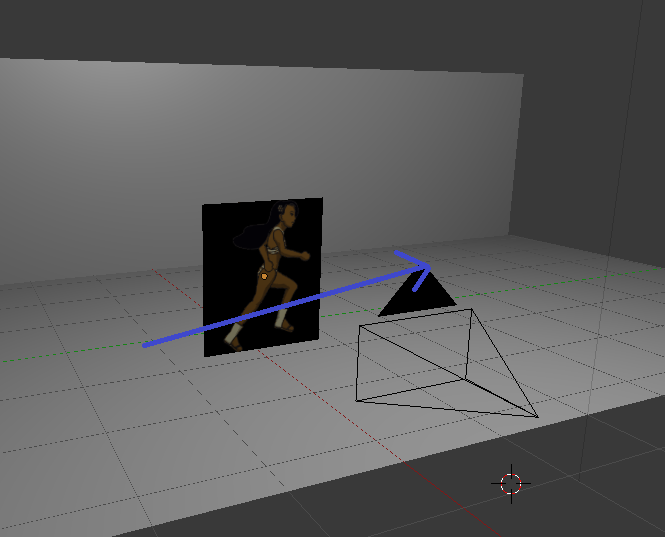
\includegraphics[width=0.7 \textwidth]{Imagenes/camara01}}
   \subfigure[Seguimiento vertical.]{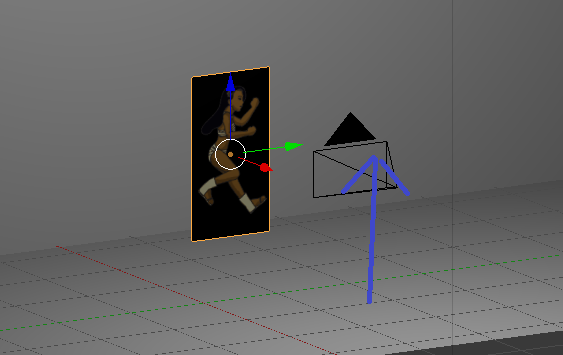
\includegraphics[width=0.7 \textwidth]{Imagenes/camara02}}
  \caption{La cámara seguirá la posición del jugador en el eje x y y.}
  \label{fig:Camara}
\end{figure} 
	\subsection{Periféricos}
	Patalla táctil.
	\subsection{Controles}
	Del lado izquierdo inferior de la pantalla existirán cuatro botones: dos botones de desplazamiento, uno de salto y otro de disparo.Todos estos botones son de forma circular y en conjunto ocupan un cuarto de la pantalla (ver figura \ref{fig:Controles}). A continuación se describirá cada botón y su funcionamiento.
	\begin{itemize}
		\item \textbf{Botón moverse derecha:} Botón cuyo icono es una flecha apuntando hacia la derecha. Permite al personaje jugable desplazarse hacia la derecha.
		\item \textbf{Botón moverse izquierda:} Botón cuyo icono es una flecha apuntando hacia la izquierda. Permite al personaje jugable desplazarse hacia la izquierda.
		\item \textbf{Botón disparar:} Botón cuyo icono es una flama girada noventa grados en sentido contrario de las manecillas del reloj. La acción de este botón depende de la cantidad de tonalli del personaje jugable. Cuando ésta es mayor a cero, el jugador dispara esferas de energía que desaparecen después de determinado tiempo. Estas esferas de energía pueden efectuar una cantidad de daño en los enemigos de cada nivel pero no tienen efecto sobre los obstáculos. Cada disparo decrementa la cantidad de tonalli total de manera constante, cuando ésta llega a cero el jugador no podrá realizar ningún disparo hasta que se recargue la barra de cantidad de tonalli(la cual tiene un tiempo de recarga automática una vez que llega a cero) o toque el item de flor de vainilla.
		\item \textbf{Botón saltar:} El icono de este botón es una flecha que apunta hacia arriba. Este botón solamente se puede accionar dos veces seguidas, es decir permite hacer de manera consecutiva dos saltos.  
	\end{itemize}
	\begin{figure}
  \centering
  \subfigure[Acción del botón de moverse derecha.]{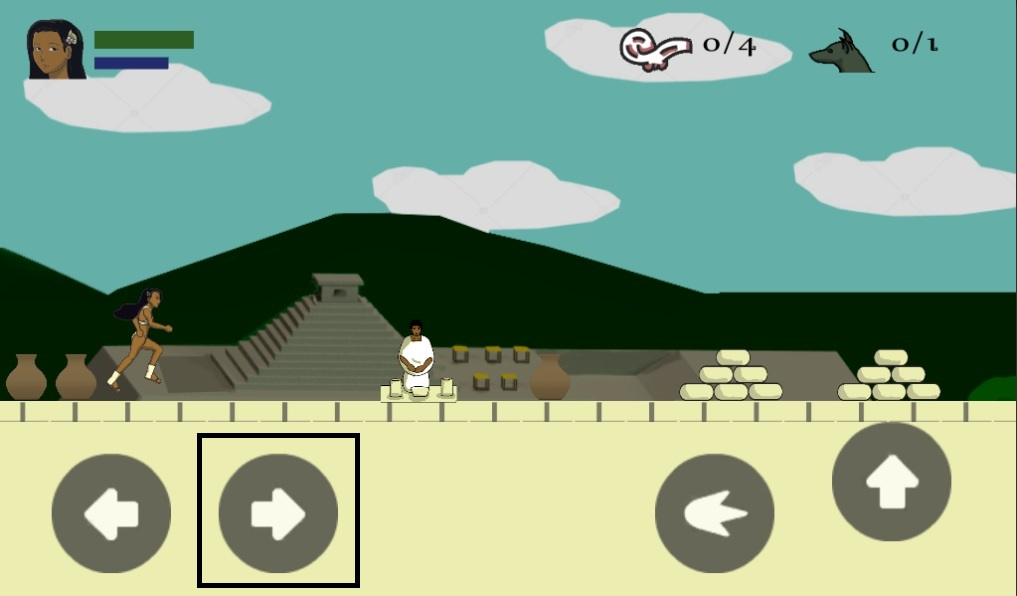
\includegraphics[width=0.45 \textwidth]{Imagenes/ControlCorrerDerGUI}}
   \subfigure[Acción del botón de moverse izquierda.]{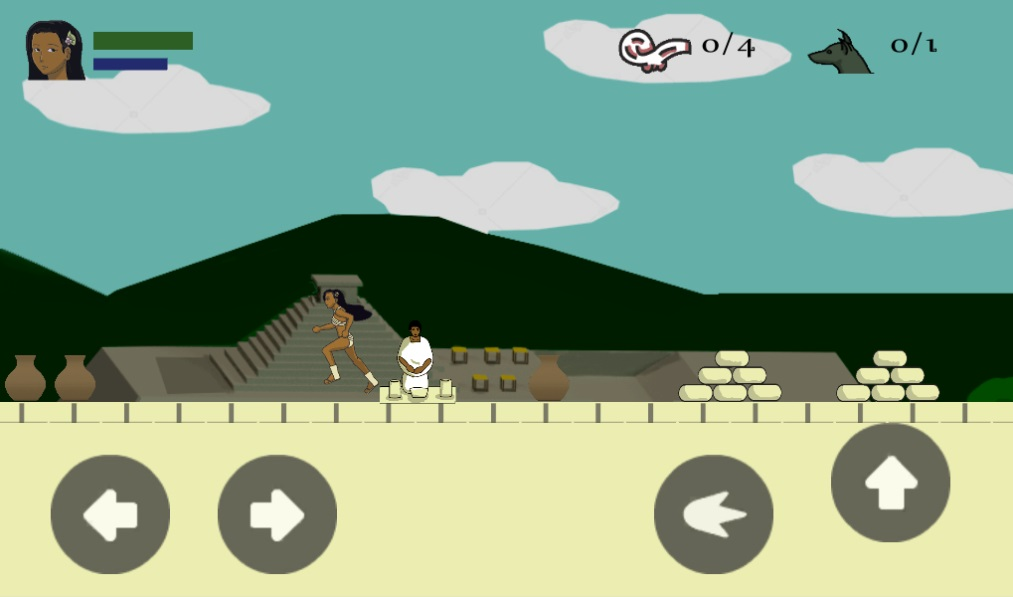
\includegraphics[width=0.45 \textwidth]{Imagenes/ControlCorrerIzq}}
   \subfigure[Acción del botón de disparar.]{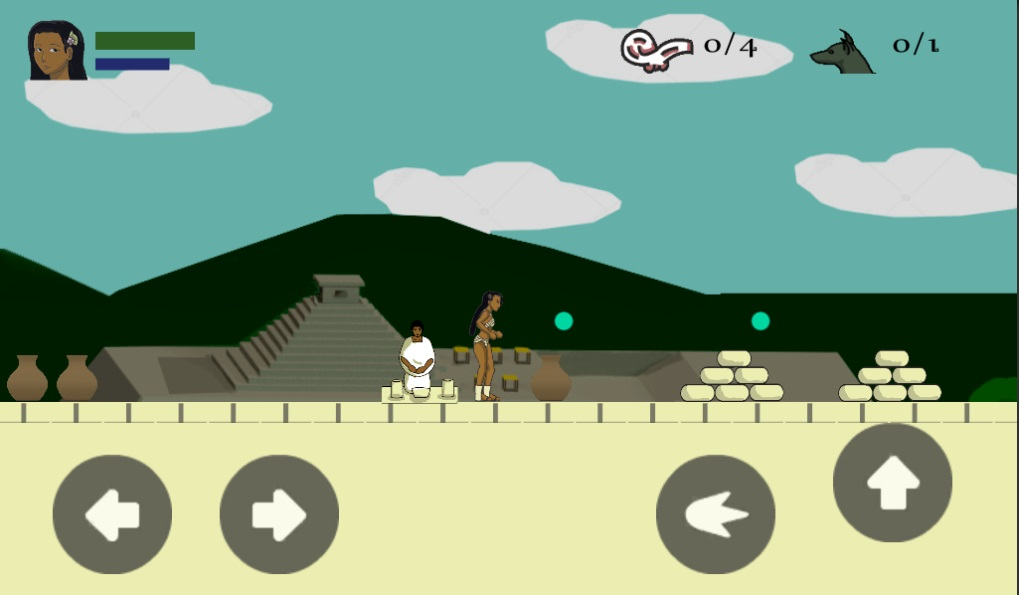
\includegraphics[width=0.45 \textwidth]{Imagenes/Controldispara}}
   \subfigure[Acción del botón de saltar.]{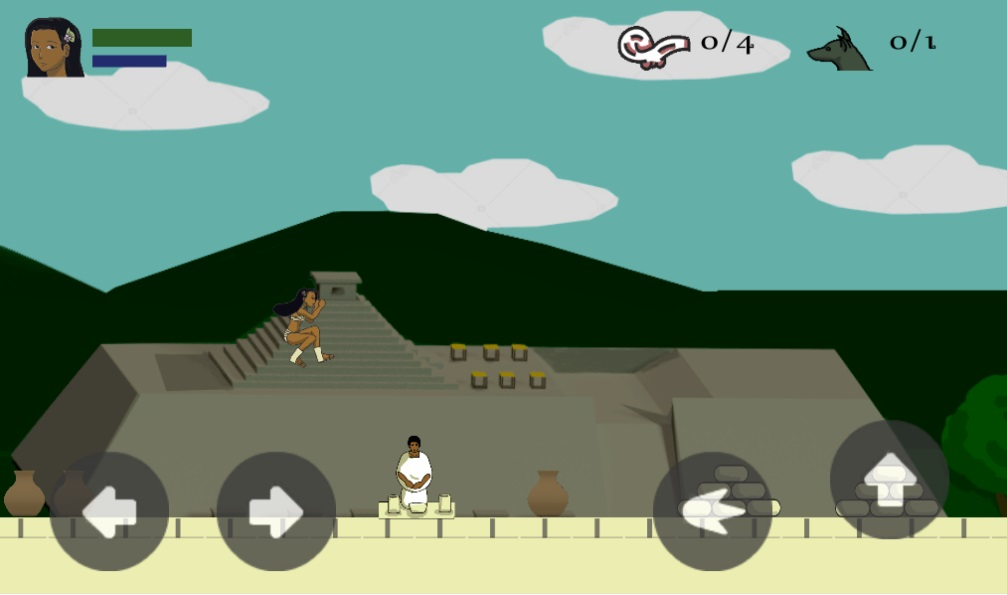
\includegraphics[width=0.45 \textwidth]{Imagenes/ControlSalta}}
  \caption{Acciones que desencadena cada botón.}
  \label{fig:Controles}
\end{figure} 
	\subsection{Guardar/Cargar}
Dentro del juego existen dos tipos de guardado en el juego: el guardado automático y el checkpoint. Y uno que guarda las estadísticas del personaje.
\begin{itemize}
\item \textbf{Guardado automático}: 
Este tipo de guardado se realizará cada vez que el jugador haya completado un nivel o una cinemática.
A la vez que desbloqueará la cinemática o el nivel siguiente a jugar.
La partida se carga en la ventana donde se muestran todos los niveles (recordando que según sea el avance del jugador estarán bloqueados o no). En esta ventana se muestra los cuadros a cargar con una imagen a seleccionar las cinemáticas y niveles de manera cronológica respecto al juego.
Este control esta a cargo de una clase llamada MenuLevelController que contiene un registro de las escenas por nombre y si de esta ya ha sido jugada o no y dentro del nivel el progreso lo manejará con el archivo respectivo de avance del nivel.
\item \textbf{Checkpoint}: 
El número de checkpoints será diferente por cada nivel.
Este tipo de guardado permitirá al jugador reiniciar el nivel desde un determinado punto. El jugador podrá activar el checkpoint si logra tocar los puntos donde existen búhos (ver \ref{per.buho}). Este guardado mantendrá la posición del jugador en un nivel en especifico. Es decir, el personaje al morir se posicionará solo en el checkpoint que haya activado inmediatamente antes. 
Cada que muere se mantendrá el puntaje, progreso del personaje que lleve y también cada cambio que exista dentro del nivel siempre y cuando esté dentro del nivel, de lo contrario si sale del nivel la variable asignada en checkpoint volverá a ser su valor por default, que sería el primer checkpoint o posición más cercana al inicio del nivel.
\item \textbf{Personaje}: 
El personaje a medida que avance en el juego tiene la posibilidad de incrementar sus características (la vida y poder de daño). Dichas características están en un archivo denominado como status player.
Este avance de características será permanente a lo largo del juego. Si el avance del juego no se guarda, tampoco las características del personaje. Este registro de características será visible en la ventana de ingreso al nivel, en la parte superior izquierda.
			Ver figura \ref{fig:statusPlayer}.
			\begin{figure}
				\centering
				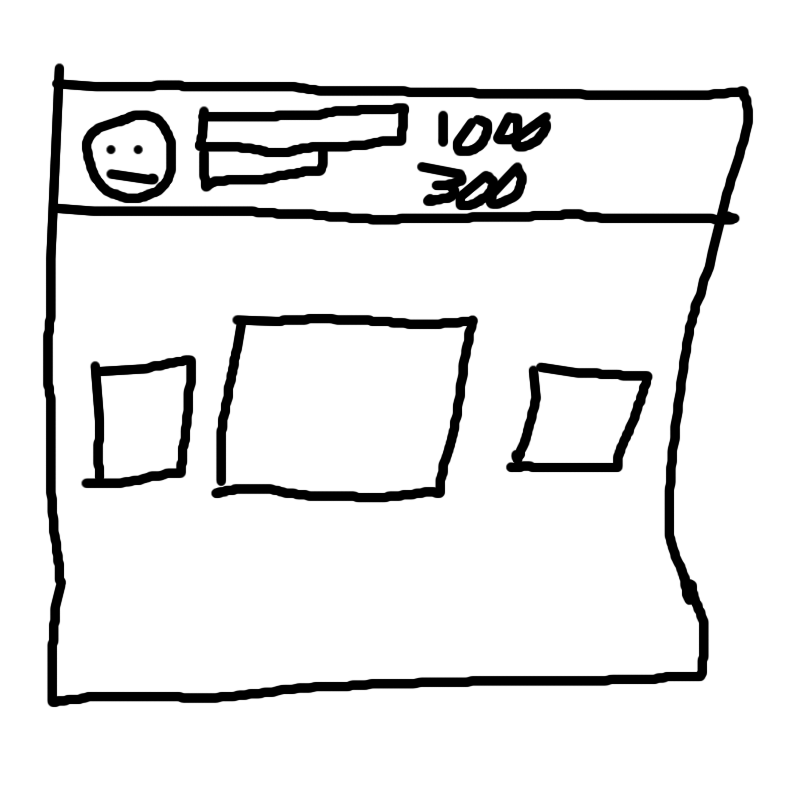
\includegraphics[height=0.2 \textheight]{Imagenes/statusPlayer}
				\caption{Estatus del player en ventana.}
				\label{fig:statusPlayer}
			\end{figure}
\end{itemize}
	
\section{Estados del juego}
Ver figura \ref{fig:EstadosJuego}
\begin{figure}
  \centering
     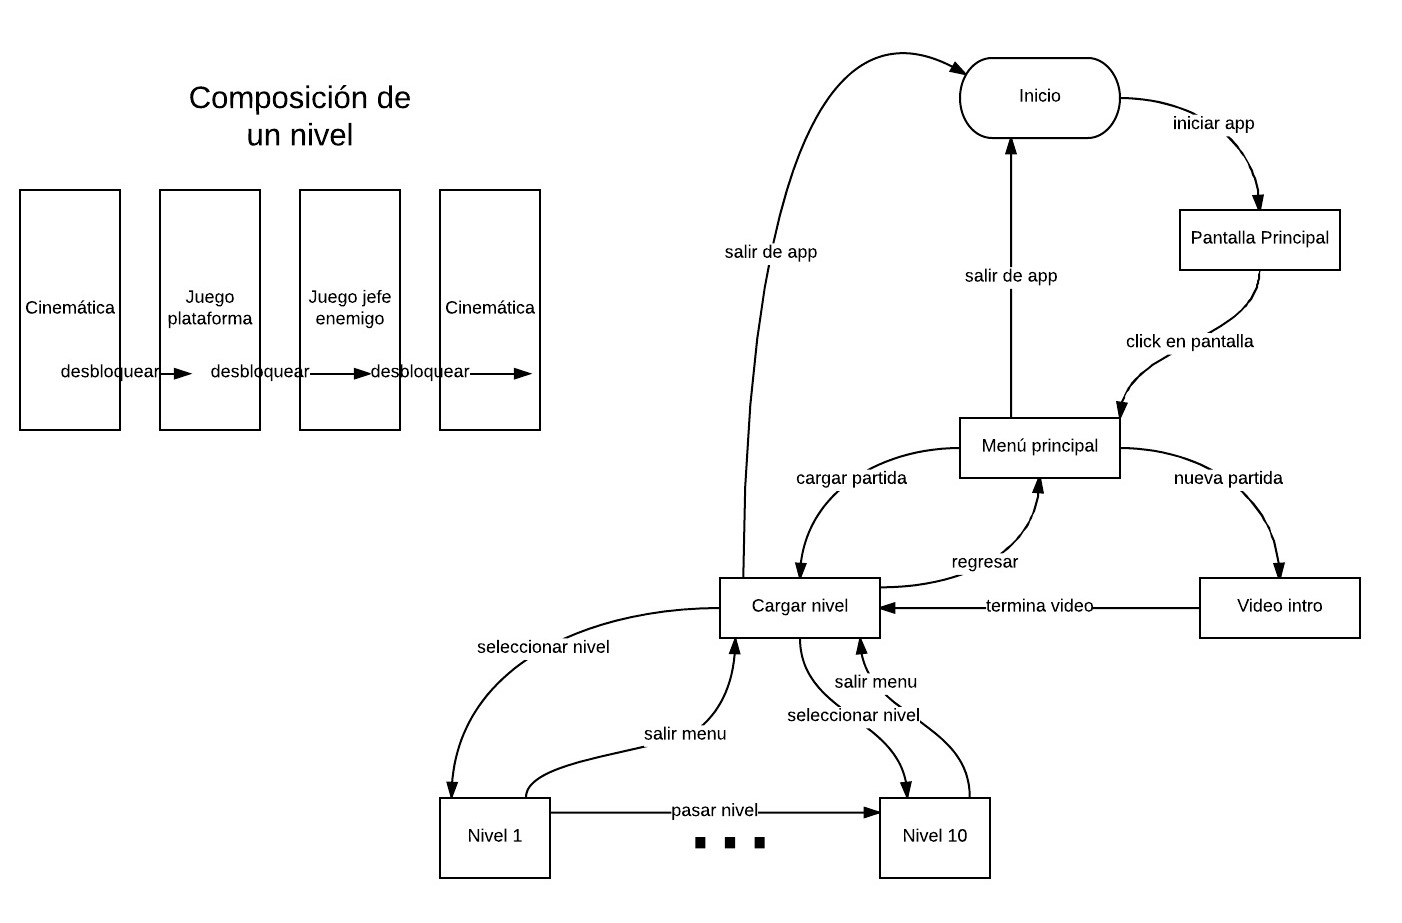
\includegraphics[width=\linewidth]{Imagenes/estadosJuego}
  \caption{Progreso del juego}
  \label{fig:EstadosJuego}
\end{figure} 


\section{Interfaces}
	\subsection{Interfaz 1.00 Pantalla de inicio.}
	\subsubsection{Descripción de la pantalla}
Todos los elementos se encuentran centrados en esta pantalla. En la parte centro superior se encuentra el logotipo del juego. Abajo de éste, se puede leer el mensaje: "Toque la pantalla para empezar". Al pie de la pantalla se puede ubica la información de derechos de autor del juego.
	\subsubsection{Estados del juego}
Es el estado inicial del juego.
Al tocar la pantalla se muestra la Interfaz 2.0
	\subsubsection{Imagen}
\begin{figure}
  \centering
   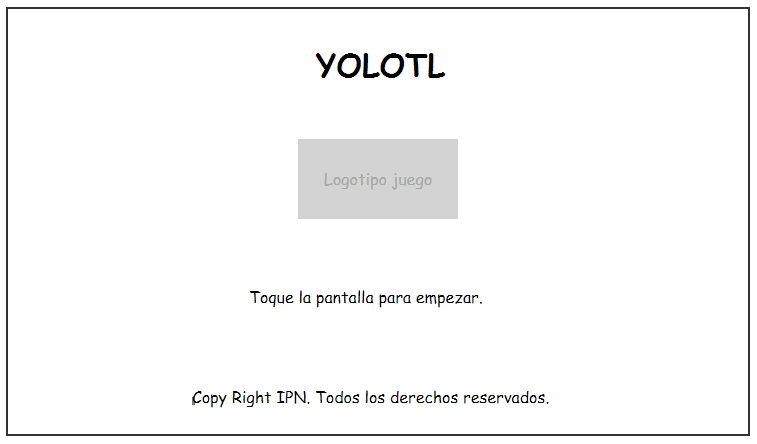
\includegraphics[width=0.6 \textwidth]{Imagenes/interfaz00}
  \caption{Interfaz 1.0 Pantalla de inicio.}
  \label{fig:PInicio}
\end{figure} 

Ver figura \ref{fig:PInicio}


\subsection{Interfaz 2.00 Menú principal.}
	\subsubsection{Descripción de la pantalla}
El logotipo del juego se muestra en la parte superior derecha de la pantalla. En la parte inferior izquierda se muestran las dos opciones: Nueva partida, Cargar partida. De fondo se muestra la misma Imagen que en la interfaz 01.00. 
Cada opción desencadena un cuadro de dialogo en donde el usuario debe de confirmar la acción que va desea ejecutar.
	\subsubsection{Estados del juego}
La interfaz 2.01 contiene los siguientes botones:
\begin{itemize}
	\item \textbf{Nueva partida}:  Dirige a la presentación de la cinemática introductoria del juego.
	\item \textbf{Cargar partida}: Dirige a la interfaz 3.00 en caso de que exista una partida previamente guardada, en caso contrario abre un cuadro de dialogo en donde se le dice al Jugador que no existe partidas que cargar.
\end{itemize}
Se puede llegar a esta Interfaz a partir de la Interfaz 01.00 
	\subsubsection{Imagen}
Ver figura \ref{fig:PMenuP}
\begin{figure}
  \centering
   \subfigure[Menú principal] {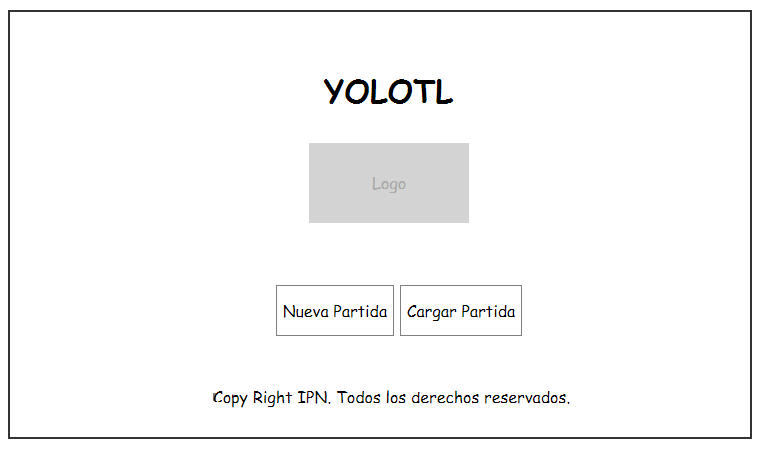
\includegraphics[width=0.6 \textwidth]{Imagenes/interfaz01}}
   
 	\subfigure[Cuadro de dialogo para confirmar iniciar nueva partida.] {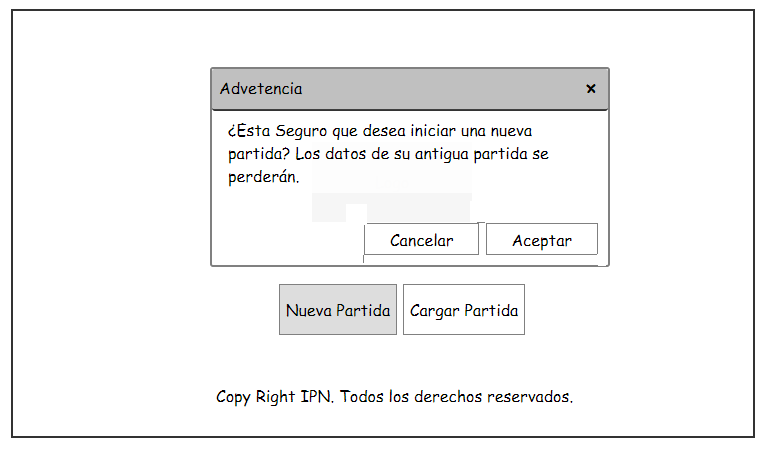
\includegraphics[width=0.6 \textwidth]{Imagenes/interfaz01_02}}
 	
\subfigure[Cuadro de dialogo cuando no existen partidas que cargar.] {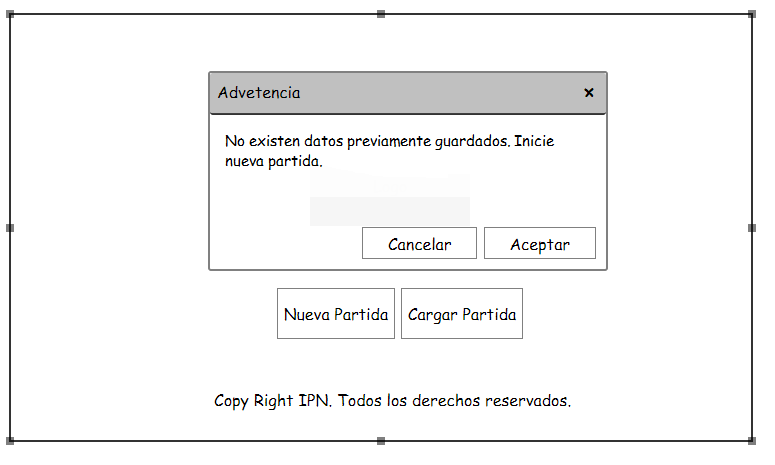
\includegraphics[width=0.6 \textwidth]{Imagenes/interfaz01_03}}
  \caption{Interfaz 2.00 Menú principal.}
  \label{fig:PMenuP}
\end{figure} 
 

\subsection{Interfaz 3.00 Selección de nivel}
	\subsubsection{Descripción de la pantalla}
Muestra el nombre de la pantalla en la esquina superior izquierda.
Los iconos de nivel están organizados en un carrusel que permite la selección de un nivel en especifico siempre y cuando el Jugador lo haya desbloqueado anteriormente.  
Bajo el carrusel se encuentra un apartado donde se podrá visualizar información del nivel, tal como el nombre y una breve descripción.
Del lado derecho de la sección donde se muestra la información del nivel 
	\subsubsection{Estados del juego}
Se llega a esta interfaz a través de la interfaz 2.00, siempre que el Jugador oprima el botón de cargar partida.
La interfaz 3.0 cuenta con los siguientes botones:
\begin{itemize}
	\item \textbf{Iniciar Nivel}: Envía al inicio del nivel seleccionado.
	\item \textbf{Control de carrusel}: estos botones permite controlas los elementos que se almacenan en el carrusel.
\end{itemize} 
	\subsubsection{Imagen}
	Ver figura \ref{fig:SelNivel}
\begin{figure}
  \centering
   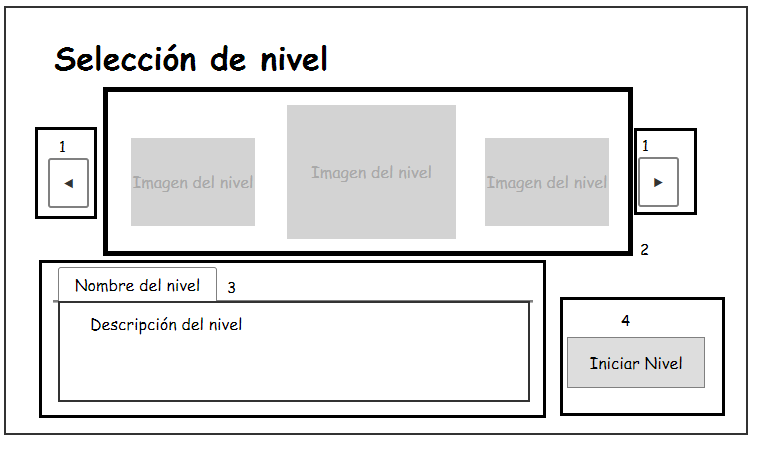
\includegraphics[width=0.6 \textwidth]{Imagenes/interfaz02_01}
  \caption{Interfaz 2.00 Selección de nivel.1 botones que controlan el carrusel. 2 Carrusel. 3 Información del nivel seleccionado. 4 Botón Iniciar nivel.}
  \label{fig:SelNivel}
\end{figure} 
 
	\section{Niveles}
\subsection{Nivel 1}
	\subsubsection{Título del nivel}
	La chica y el perro.
	\subsubsection{Encuentro}
Nivel introductorio que le permite al jugador familiarizarse con las mecánicas básicas de juego: saltar, moverse y abrir y cerrar cuadros de dialogo. Además, este nivel servirá para mostrar el contexto histórico en el que se sitúa el argumento del juego.
	\subsubsection{Descripción}
	\begin{itemize}
		\item\textbf{Tianguis}: El jugador controlará a Malinalli y recorrerá un mercado, en donde podrá dialogar con diferentes NPCS. Xólotl le robara un carta a Malinalli.
		Dentro del tianguis existen ciudadanos, cada uno el jugador al acercarse a una distancia predeterminada de ellos se le da la opción para que pueda comunicarse con ellos. Esto se ve al desplegarse un símbolo (representando la opción de poder dialogar) en la parte superior del ciudadano a hablar cuando uno se aproxima, así el jugador se le notifica que puede apretar el botón (ahora con el mismo símbolo) de diálogo, luego se despliega un recuadro adicional que contiene la información, para cerrar este recuadro y continuar se debe volver a oprimir el botón de diálogo.
		Ver figura \ref{fig:simboloDialogo}.
		\begin{figure}
			\centering
			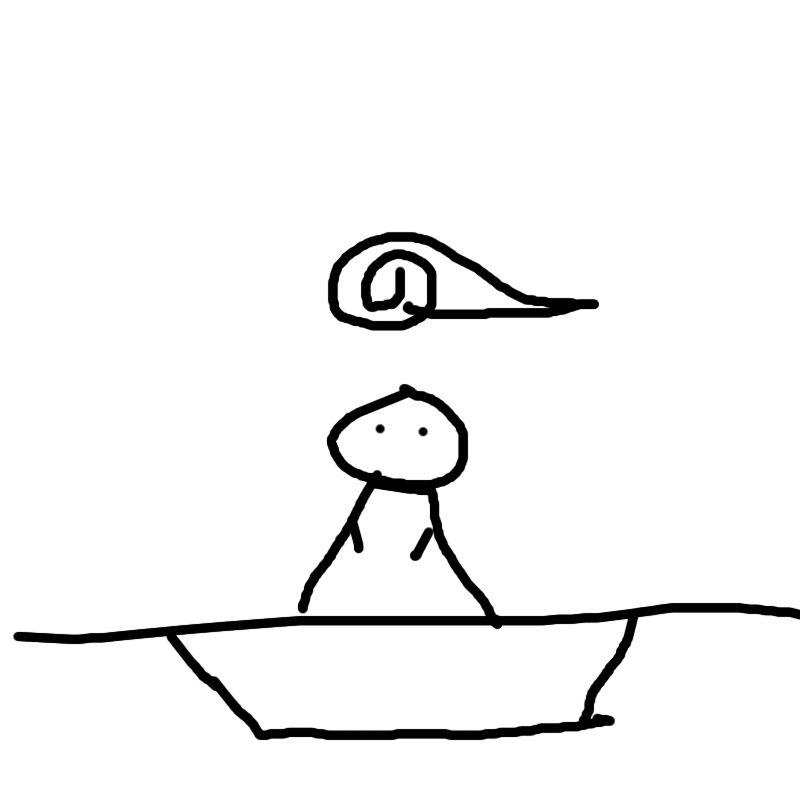
\includegraphics[height=0.2 \textheight]{Imagenes/simboloDialogo}
			\caption{Símbolo de diálogo sobre el ciudadano.}
			\label{fig:simboloDialogo}
		\end{figure}
		Ver figura \ref{fig:cuadroDialogo}.
		\begin{figure}
			\centering
			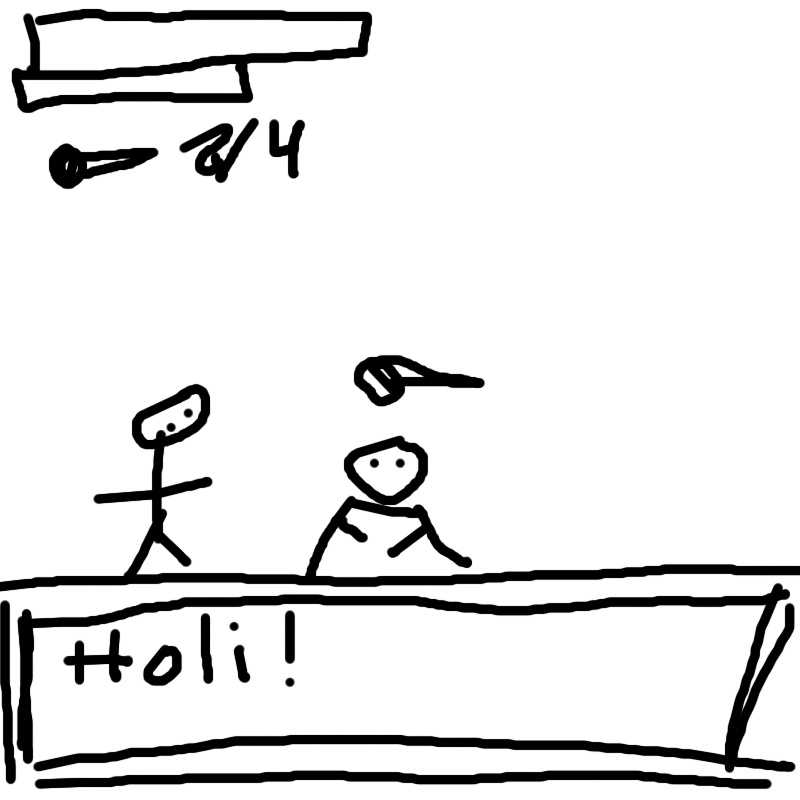
\includegraphics[height=0.2 \textheight]{Imagenes/cuadroDialogo}
			\caption{Recuadro de diálogo.}
			\label{fig:cuadroDialogo}
		\end{figure}
		\item\textbf{Selva}: Ella tendrá que perseguir a Xolotl por la selva, al final Xolotl adoptará la forma de un jaguar. Xólotl utiliza este encuentro para probar la valentía de Malinalli ante situaciones en las que se encuentre en peligro, pero sin la oportunidad de defenderse.    
		Para ello el jugador cada que se aproxime a una distancia determinada del perro, el perro se desplaza en dirección horizontal a otra zona más adelante. Así hasta que el jugador accede a una zona diseñada para que no pueda escapar (como un agujero). Luego continua con la cinemática donde el perro se convierte en un jaguar para probar su valor.
		Ver figura \ref{fig:proximidadPerro}.
		\begin{figure}
			\centering
			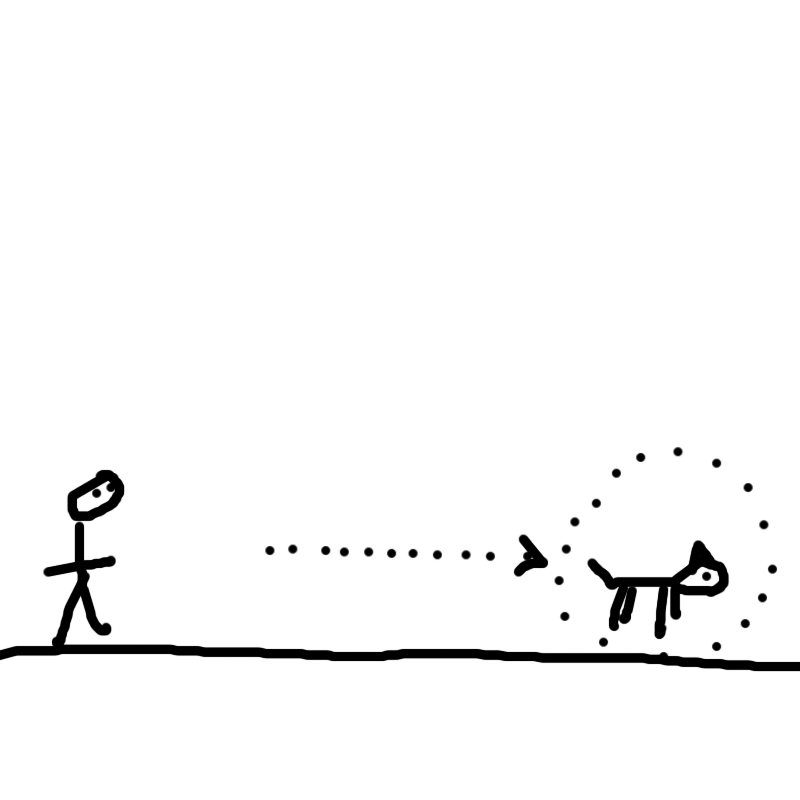
\includegraphics[height=0.2 \textheight]{Imagenes/proximidadPerro}
			\caption{Interacción del perro con le jugador.}
			\label{fig:proximidadPerro}
		\end{figure}
	\end{itemize}

	\subsubsection{Objetivos}
\begin{itemize}
	\item \textbf{Tianguis}:
	El jugador deberá de activar al menos cuatro diálogos para poder desbloquear la infección con Xólotl y que se active la cinemática donde éste le roba el objeto a Malinalli.
	Para que el jugador pueda ver cuantos diálogos está activando, se mostrará en la ventana del lado superior izquierdo un contador con símbolo y después "x/4", siendo "x" el número de diálogos que se activen y "4" el número de de diálogos que el jugador debe activar antes de avanzar al siguiente apartado.
				Ver figura \ref{fig:ventanaSimboloDialogo}.
				\begin{figure}
					\centering
					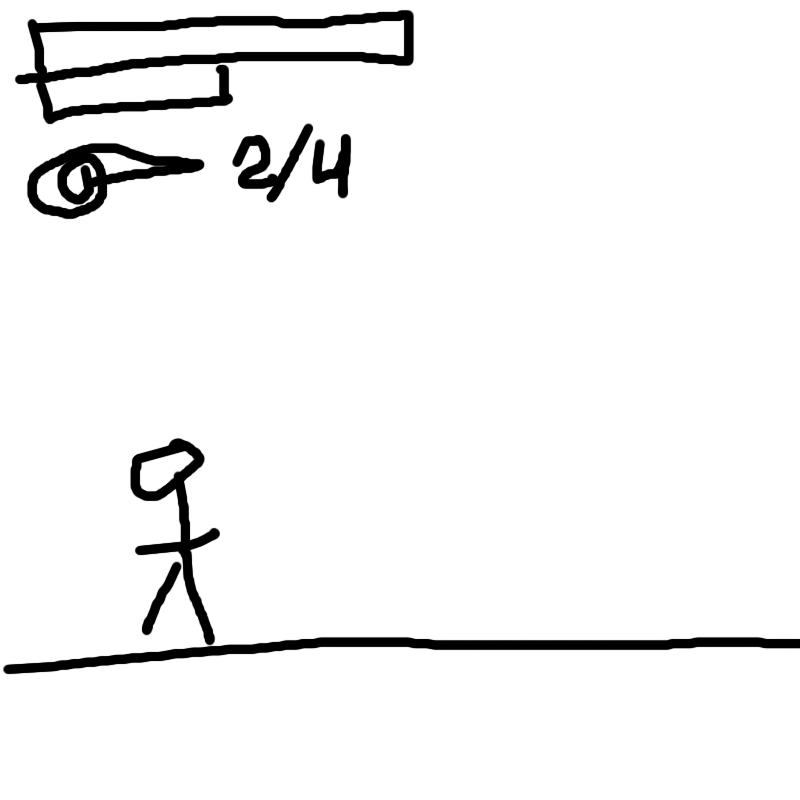
\includegraphics[height=0.2 \textheight]{Imagenes/ventanaSimboloDialogo}
					\caption{Símbolo de diálogo en la ventana.}
					\label{fig:ventanaSimboloDialogo}
				\end{figure}
	\item \textbf{Selva}: El jugador deberá de seguir a Xólotl. Durante la persecución deberá de superar obstáculos y plataformas saltándolos. Obtener la caracola.
\end{itemize}
	\subsubsection{Progreso}
	Al concluir el nivel el jugador:
\begin{itemize}
	\item El jugador podrá ver las siguientes cinemáticas (Consultar el guión literario del juego):
	\begin{itemize}
		\item Cinemática 3.
		\item Cinemática 4.
	\end{itemize}
\item Desbloqueará el segundo nivel del juego.
\item Obtendrá el objeto caracola con lo que se habilitará el botón de disparo en la interfaz gráfica del juego.
\end{itemize}
	\subsubsection{Enemigos}
Al ser un nivel introductorio de mecánicas de juego no orientadas al combate, el nivel no cuenta con enemigos.
	\subsubsection{Items}
Ningún item utilizable.
	\subsubsection{Personajes}
\begin{itemize}
\item Malinalli (Personaje jugable).
	\begin{itemize}
		\item Animación correr.
		\item Animación saltar. 
		\item Animación normal. 
	\end{itemize}	
\item Xólotl.
	\begin{itemize}
		\item Xoloitzcuintle.
			\begin{itemize}
				\item Animación correr.
				\item Animación normal. 
		\end{itemize}	
		\item Jaguar.
			\begin{itemize}
				\item Animación correr.
				\item Animación normal. 
		\end{itemize}	
	\end{itemize}	

\item NPC. Ver ciudadanos en \ref{per.ciudadanos}.
	\begin{itemize}
		\item Mujer comerciante. 
			\begin{itemize}
				\item Animación mover mercancía de un lado a otro.
			\end{itemize}
		\item Mujer jarrón.
			\begin{itemize}
				\item Animación caminar.
			\end{itemize}			 
		\item Hombre jarrón.
			\begin{itemize}
				\item Animación caminar.
			\end{itemize} 
		\item Hombre cacao.
			\begin{itemize}
				\item Animación caminar.
			\end{itemize}
		\item Hombre noble.
			\begin{itemize}
				\item Animación revisar mercancía(Si esta cerca de un puesto). 
				\item Animación platicar (Si esta cerca de otro noble).
				\item Animación contar granos de cacao (Si no esta cerca de un puesto o de un noble).
			\end{itemize}				
	\end{itemize}	 
\end{itemize}
\subsubsection{Escenario}
\begin{itemize} 
	\item Fondo:
\begin{itemize}
			\item Ciudad de \ref{Centla}: Se ve el templo a la lejanía y unas casas. Este fondo se usará en la etapa del tianguis del nivel.
			\item Selva: La ciudad se ve más alejada, hay árboles en un plano más cercano. Este fondo se utilizará en la etapa de la selva  
\end{itemize}	
	\item Suelo:
		\begin{itemize}
			\item Suelo pavimentado: Será usado en el tianguis.
			\item Suelo con pasto: Será usado en la selva.
		\end{itemize}
	\item Obstáculos:
		\begin{itemize}
			\item Tianguis
				Sin obstáculos.
			\item Selva
				\begin{itemize}
					\item Caja. Ver en \ref{obs.caja}.
					\item Sacos Cacao. Ver en \ref{obs.saco}.
				\end{itemize}
		\end{itemize}
	\item Objetos de fondo:
		\begin{itemize}
			\item Tianguis
				\begin{itemize}
					\item Jarron
					\item Saco de cacao
					\item Sacos de cacao apilados
				\end{itemize}
			\item Selva
				\begin{itemize}
					\item Arbusto
				\end{itemize}

		\end{itemize}
\end{itemize}	
\subsubsection{Música y efectos de sonido}
\begin{itemize} 
\item Temas del juego: El juego se Música lizará con orquesta.
\begin{itemize}
		\item La música de fondo que suena en el mercado debe de evocar un sentimiento de cotidianidad, seguridad y alegría. En el tema predominaran instrumentos de viento.
		\item La música en la selva debe de ser sobre inicio de un viaje. Debe de evocar en el jugador el deseo de aventura y a la vez hacerlo sentir que está en un lugar conocido.
		\item La música cuando Xólotl le habla a Malinalli debe de ser un tema que se ajuste con la personalidad del Dios ya que será el tema que sonara cuando él tenga diálogos importantes que decir, así que debe ser un tema que muestre determinación y misterio.
\end{itemize} 
\item Efectos de sonido:
	\begin{itemize}
		\item Gente: Efecto sonóro de fondo de gente hablando y caminando en el tianguis
		\item Pasos: Este efecto se activará cuando Malinalli camine.
		\item Viento: Este efecto sonara cuando Malinalli se encuentra con el jaguar.
		\item Ladrido: Este efecto sonara cuando Xólotl le robe el objeto a Malinalli.
\end{itemize}
\end{itemize}
\subsubsection{Referencia a BGM y SFX}
\begin{itemize}
	\item Un efecto de luz especial cuando Xólotl se transforma de jaguar a xoloitzcuintle.

\end{itemize}



	
		\subsection{Nivel 2}
	\subsubsection{Título del nivel}
	Apanohuaia:"Lugar en que habita el perro"
	\subsubsection{Encuentro}
El nivel le enseñara al jugador las mecánicas de combate: combate simple contra enemigos y el combate contra un jefe. 
	\subsubsection{Descripción}
Malinalli y Xólotl se adentran al inframundo. Su primer reto a superar será cruzar el río de Apanohuaia y sus peligros para poder derrotar al primer guardián del inframundo: la iguana gigante Xochitonal. Xólotl adopta la forma de un ajolote de gran tamaño para que ambos puedan cruzar el río, por lo que el jugador controlara al Sprite de Malinalli sobre un ajolote de gran tamaño. 
	\subsubsection{Objetivos}
\begin{itemize}
	\item Aprender a utilizar el funcionamiento de los ataques de Malinalli y de los ítems de curación.
	\item El jugador deberá de atravesar el lago derrotando a los enemigos que encuentre en el camino. Para derrotar a los enemigos el jugador disparará tonalli.
	\item El jugador deberá evitar tocar los Xoloitzcuintles que hay en todo el nivel. La cantidad en la que se incrementa el daño que puede infringir Xochitonal y el numero de Xoloitzcuintles tocados se mostraran en la parte superior derecha de la pantalla (Ver figura \ref{fig:GUICtrlNivel2}). Una vez que el jugador hace contacto con un Xoloitzcuintle, el Xoloitzcuintle desaparecera y se incrementara en uno el indicador de la cantidad de Xoloitzcuintles tocados y el indicador de la cantidad de daño que puede efectuar Xochitonal (Ver figura \ref{fig:InterNivel2}). 
	\item El jugador deberá vencer al guardián del primer nivel del inframundo, Xochitonal.
\end{itemize}


\begin{figure}
  \centering
   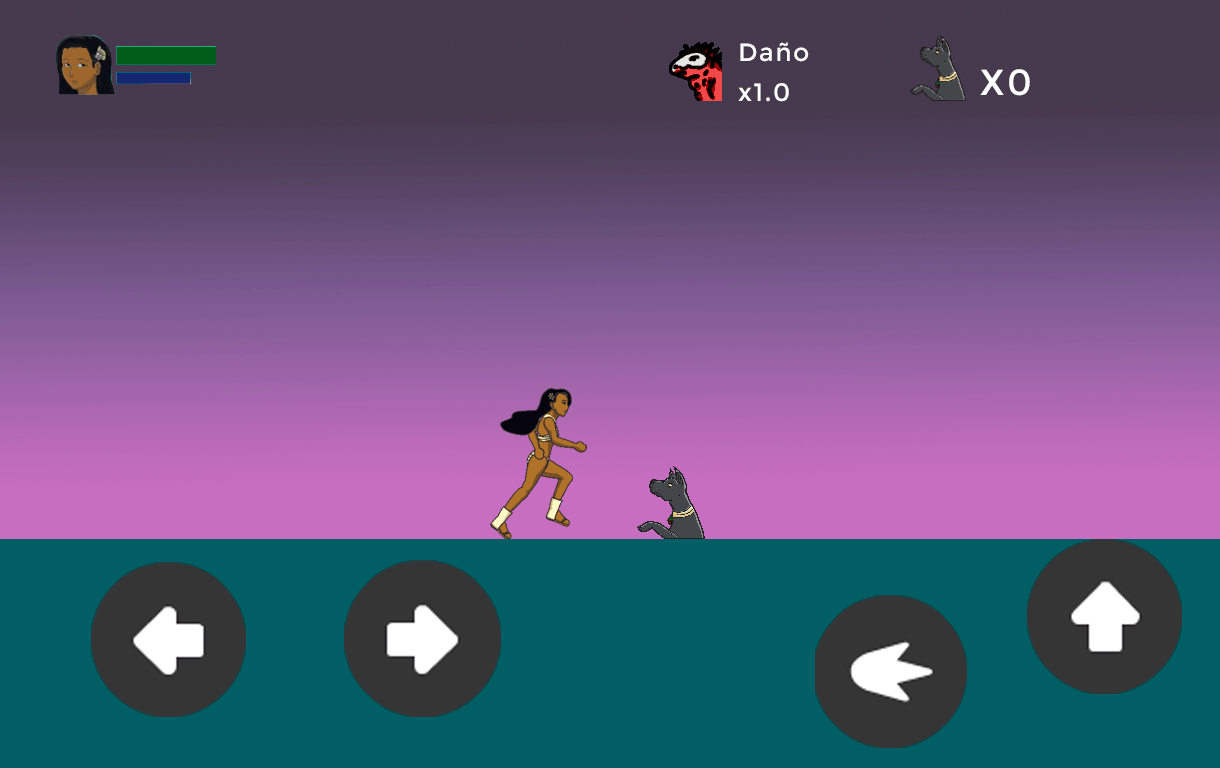
\includegraphics[width=0.4 \textwidth]{Imagenes//nivel02_xolo}
  \caption{1. Indicador de la cantidad de daño que puede efectuar Xochitonal. 2. Indicador de la cantidad de Xoloitzcuintles tocados.}
  \label{fig:GUICtrlNivel2}
\end{figure} 

\begin{figure}
  \centering
   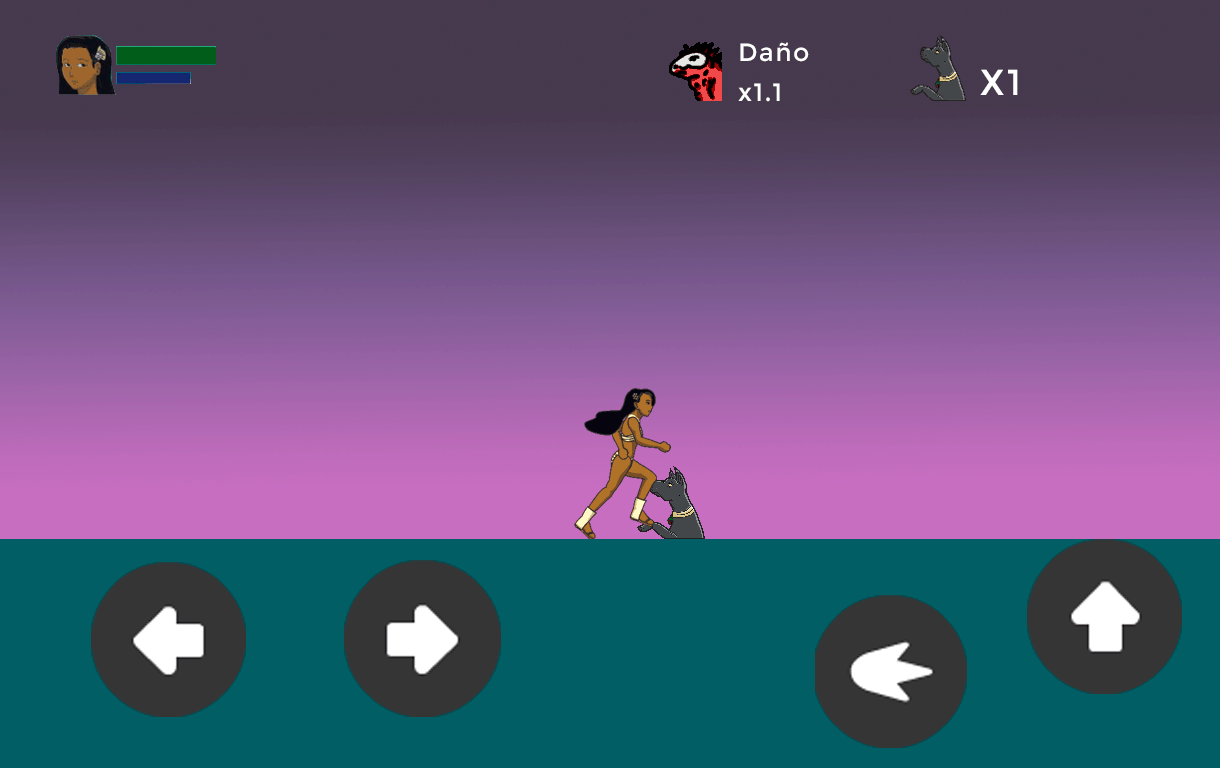
\includegraphics[width=0.4 \textwidth]{Imagenes//nivel02_xoloContacto}
  \caption{Cuando el jugador hace contacto con un Xoloitzcuintle los indicadores se modifican.}
  \label{fig:InterNivel2}
\end{figure} 

	\subsubsection{Progreso}
Al final del nivel el jugador:
\begin{itemize}
	\item Obtendrá una mejora en la cantidad de vida de Malinalli.
	\item El jugador podrá ver las siguientes cinemáticas(Para mayor información sobre cada una, ver el guion literario del juego)
		\begin{itemize}
			\item Cinemática 6.
			\item Cinemática 7.
			\item Cinemática 8.
			\item Cinemática 9.
			\item Cinemática 10.
		\end{itemize}
	\item Tendrá disponible el tercer nivel del juego. 
\end{itemize}
	\subsubsection{Enemigos}
	\begin{itemize}
		\item Fantasma rojo. Ver en \ref{per.fantasmaR}.
			\begin{itemize}
				\item Animación fuego.
				\item Animación disparo.
			\end{itemize}
		\item Fantasma morado. Ver en \ref{per.fantasmaM}.
			\begin{itemize}
				\item Animación fuego.
			\end{itemize}
		\item Piedras filosas. Ver en \ref{obs.piedrasF}.
		\item Xochitonal. Ver en \ref{per.xochitonal}.
			\begin{itemize}
				\item Animación emerge del agua.
				\item Animación se sumerge en el agua.
				\item Animación Dispara burbujas.  
				\item Animación es herido.
			\end{itemize}
	\end{itemize}
	\subsubsection{Items}
	\begin{itemize}
		\item Xoloitzcuintles.
		\item Grano de cacao.
		\item Flor de vainilla.
	\end{itemize}
	\subsubsection{Personajes}
	\begin{itemize}
		\item Malinalli. Ver en \ref{per.malinalli}.
		\begin{itemize}
			\item Animación correr.
			\item Animación saltar.
			\item Animación correr con caracola.
			\item Animación saltar con caracola.
			\item Animación normal.
			\item Animación recibir daño.
			\item Animación morir.
		\end{itemize}
		\item Xolotl (ajolote). Ver en \ref{per.xolotl}.
			\begin{itemize}
				\item Animación salto.
				\item Animación normal/nado.
			\end{itemize}
		\item Xochitonal. Ver en \ref{per.xochitonal}.
	\end{itemize}
	
\subsubsection{Escenario}
\begin{itemize} 
	\item Fondo:
Montañas en el plano más alejado, y a sus pies una pequeña linea que muestre la orilla del río. El cielo es de color verde en degradado con negro.
	\item Suelo:
		\begin{itemize}
			\item Agua: Será utilizada durante la zona de plataformas y durante la batalla contra el jefe del nivel.
			\item Suelo con pasto: Será usado durante la cinemática 4 y la cinemática 8.
		\end{itemize}
	\item Obstáculos:
		\begin{itemize}
			\item Piedras filosas. Ver en \ref{obs.piedrasF}.				
		\end{itemize}
	\item Objetos de fondo: 
	\\
	\par	
	Sin objetos de fondo.
	
\end{itemize}	
	
	\subsubsection{Música y efectos de sonido}
\begin{itemize}
	\item Temas del juego:
		\begin{itemize}
			\item La Música lización que corresponde a la zona de enemigos normales de este nivel debe de reflejar que uno se encuentra en la entrada de un lugar misterios y peligroso, pero de gran carga espiritual (Por lo que se recomienda alguna canción que contenga coros, los coros preferiblemente deben de estar en Náhualt y deben de hablar sobre el sufrimiento de las almas que no pudieron cruzar).
			\item La música que acompaña a la batalla con Xochitonal debe de hacer sentir peligro que se está luchando por sobrevivir pero sin perder la carga espiritual que conlleva este nivel.
		\end{itemize}
	\item Efectos de sonido:
		\begin{itemize}
			\item sonido de explosión de agua: Este sonido se usara para los ataques de Xochitonal.
			\item Sonido de salpicadura de agua: Sonido cuando Xolotl salta y aterriza en el agua. 
		\end{itemize}
\end{itemize}
	\subsubsection{Referencia a BGM y SFX}
\begin{itemize}
	\item Oleaje: este efecto se hará en el agua cuando Xochitonal emerge o se sumerge en el río.
	\item Salpucadura de agua: Efecto que aparecerá cuando Xólotl salta o aterriza en el agua.
	\item Explosión de burbuja: Efecto cuando el ataque de burbujas de Xochitonal hace contacto con algo.
	\item Explosión de energía tonalli: Este efecto se presentara en dos colores:
	\begin{itemize}
		\item Explosión de energía tonalli rojo: efecto cuando los enemigos normales son derrotados.
		\item Explosión de energía tonalli rojo: Efecto cuando la cantidad de salud de Malinalli llega a cero.
	\end{itemize}	 
\end{itemize}

	
\subsection{Nivel 3}
	\subsubsection{Título del nivel}
	Tépetl Monamicyan: Lugar en que se juntan las montañas	
	\subsubsection{Encuentro}
Segundo nivel del inframundo, solo se puede acceder a él si se ha derrotado al jefe del primer nivel.
	\subsubsection{Descripción}
	Tras haber superado el primer nivel del Mictlán, Xólotl y Malinalli han llegado al Monamicyan, nivel gobernado por Tepeyóllotl. En este nivel Malinalli debera superar diferentes plataformas para llegar a la guarida de Tepeyóllotl y así obtener el poder del segundo guardían del infreamundo.
	\subsubsection{Objetivos}
	El jugador deberá:
\begin{itemize}
	\item Superar diferentes plataformas ascendentes, por lo que se requerirá de una buena coordinación para controlar los saltos del personaje.
	\item Derrotar enemigos que protegen diferentes zonas del mapa, sin morir; cada enemigo infringirá una cantidad diferente de daño.
	\item Derrotar al jefe del nivel: Tepeyóllotl. Tepeyóllotl se encontrará protegido por su armadura de piedra por lo que sus ataques serán lentos, pero infringirán gran daño.
\end{itemize}
	\subsubsection{Progreso}
Al final del nivel el jugador:
\begin{itemize}
	\item Mejorará la cantidad de energía espiritual de Malinalli lo que permitirá usar más ataques con la caracola.
	\item Podrá ver las siguienteDesbloqueara una cinemática sobre el pasado de Malinallis cinemáticas: 
		\begin{itemize}
			\item Cinemática 12.
			\item Cinemática 13.
			\item Cinemática 14.
		\end{itemize}
	\item Desbloqueara el nivel cuatro en el menú de selección de nivel.
\end{itemize} 
	\subsubsection{Enemigos}
\begin{itemize}
	\item 	Fantasma rojo. Ver en \ref{per.fantasmaR}.
		\begin{itemize}
				\item Animación fuego.
				\item Animación disparo.
			\end{itemize}
	\item Armadillo. Ver en \ref{per.armadillo}.
		\begin{itemize}
			\item Animación de sacar picos.
			\item Animación rodar. 
		\end{itemize}
	\item Roca. Ver en \ref{obs.rocas}.
		\begin{itemize}
			\item Animación romperse.
			\item Animación rodar.
		\end{itemize}
	\item Tepeyóllotl. Ver en \ref{per.tepeyollotl}. 

\end{itemize}
	\subsubsection{Items}
\begin{itemize}
	\item 	Cacao.
	\item	Flor de vainilla.
\end{itemize}
	\subsubsection{Personajes}
\begin{itemize}
	\item Malinalli. Ver en \ref{per.malinalli}.
		\begin{itemize}
			\item Animación correr.
			\item Animación saltar.
			\item Animación correr con caracola.
			\item Animación saltar con caracola.
			\item Animación normal.
			\item Animación recibir daño.
			\item Animación morir.
		\end{itemize}
	\item Xolotl. Ver en \ref{per.xolotl}.
		\begin{itemize}
				\item Animación salto.
				\item Animación normal/nado.
		\end{itemize}
	\item Tepeyóllotl. Ver en \ref{per.tepeyollotl}.
		\begin{itemize}
			\item Animación correr.
			\item Animación saltar.
			\item Animación rugir.
			\item Animación recibir daño.
			\item Animación morir.
		\end{itemize}
\end{itemize}
\subsubsection{Escenario}
\begin{itemize} 
	\item Fondo:
\begin{itemize}
	\item Bosque frondoso desde una perspectiva de tres puntos de fuga visto desde arriba. Tendra un cielo azul despejado. A lo lejos se verá una montaña muy alta, con un templo en la cima.
\end{itemize}
	\item Suelo:
		\begin{itemize}
			\item Suelo con pasto.
		\end{itemize}
	\item Obstáculos:
		\begin{itemize}
			\item Plataforma móvil. Ver en \ref{obs.plataformaM}.
			\item Plataforma débil que cae. Ver en \ref{obs.plataformaD}.
		\end{itemize}
	\item Objetos de fondo:
		\begin{itemize}
			\item Arbusto.
			\item Árbol frágil.
		\end{itemize}
\end{itemize}	
	\subsubsection{Música y efectos de sonido}
\begin{itemize}
	\item Temas del juego:
		\begin{itemize}
			\item Zona de plataformas: La Música  de este nivel debe reflejar el sentimiento de adrenalina y vértigo que lleva escalar una superficie frágil y peligrosa.
			\item Batalla contra el jefe: La batalla contra el jefe debe de mostrar un tema que evoque la misma adrenalina de peligro con el agregado de que la sensación de peligro se intensifica.
		\end{itemize}
	\item Efectos de sonido:
		\begin{itemize}
			\item Viento soplando: A momentos se escuchara este sonido de fondo mientras se sube por las plataformas.
			\item Rugido.
			\item Roca estrellandose.
			\item Pasos: Este efecto se activará cuando Malinalli camine
		\end{itemize}
\end{itemize} 
	\subsubsection{Referencia a BGM y SFX}
\begin{itemize}
	\item Explosión de energía tonalli: Este efecto se presentara en dos colores:
	\begin{itemize}
		\item Explosión de energía tonalli rojo: efecto cuando los enemigos normales son derrotados.
		\item Explosión de energía tonalli rojo: Efecto cuando la cantidad de salud de Malinalli llega a cero.
	\end{itemize}
	\item Explosion rocas: Este efecto se usará cuando cualquier objeto que este hecho de rocas, sea enemigo o ataque, colisione contra algo.
\end{itemize}

        \subsection{Nivel 4}
        \subsubsection{Título del nivel}
        Itztépetl: Montaña de obsidiana.
        \subsubsection{Encuentro}
Tercer nivel del inframundo, se desbloquea derrotando a Tepeyollótl en el tercer nivel.
        \subsubsection{Descripción}
        Luego de la huida de Tepeyollótl, Malinalli y Xólotl iniciarán una carrera contra el tiempo para poder llegar a su segunda guarida y evitar que contacte a Tezcatlipoca pero primero deberán superar el Itztépetl, hogar de Itzpapálotl. Así deberán adentrarse en las profundidades de una cueva para encontrar templo subterráneo donde se esconde Itzpapálotl. 
        \subsubsection{Objetivos}
En este nivel el jugador deberá:        
\begin{itemize}
        \item Descubrir el camino correcto hacia el templo de Itzpapálotl, el jugador podra explorar de manera horizontal y vertical el nivel.
        \item Superar las diferentes plataformas y obstáculos que hay en el laberinto. 
        \item Derrotar a los enemigos que hay en el laberinto.
        \item Derrotar a Itzpapálotl.
\end{itemize}
        \subsubsection{Progreso}
Al final del nivel el jugador:
\begin{itemize}
        \item Aumentará el valor de la salud de Malinalli.
        \item Desbloquear las siguientes cinemáticas:
		\begin{itemize}
			\item Cinemática 16.
			\item Cinemática 17.
			\item Cinemática 18.
			\item Cinemática 19.
			\item Cinemática 20.
			\item Cinemática 21.
			\item Cinemática 22.
		\end{itemize}
        \item Desbloquear El nivel 5 del juego en el menú seleccionable.
        \subsubsection{Enemigos}
                \begin{itemize}
                        \item Fantasma rojo. Ver en \ref{per.fantasmaR}. 
            \begin{itemize}
				\item Animación fuego.
				\item Animación disparo.
			\end{itemize}
                        \item Picos de obsidiana. Ver en \ref{obs.piedrasF}.
                        \item Itzpapalotl. Ver en \ref{per.itzpapalotl}.
                \end{itemize}
        \subsubsection{Items}
                \begin{itemize}
                        \item   Cacao.
                        \item Flor de Vainilla.
                \end{itemize}
        \subsubsection{Personajes}
        \begin{itemize}
                \item Malinalli. Ver en \ref{per.malinalli}.
                \begin{itemize}
                        \item Animación correr.
                        \item Animación saltar.
                        \item Animación correr caracola.
                        \item Animación saltar caracola.
                        \item Animación normal.
                        \item Animación recibir daño.
						\item Animación morir.
                \end{itemize}
                \item Xolotl.Ver en \ref{per.xolotl}.
                	\begin{itemize}
						\item Animación salto.
						\item Animación normal.
					\end{itemize}
                \item Itzpapalotl. Ver en \ref{per.itzpapalotl}.
                \begin{itemize}
                        \item Animación disparar fuego.
                        \item Animación embestida.
                        \item Animación caminar.
                        \item Animación desvanecerse.
                        \item Animación aparecer.
                \end{itemize}
        \end{itemize}
\subsubsection{Escenario}
\begin{itemize} 
        \item Fondo:
                \begin{itemize}
                        \item Zona de plataformas:
\\
\par
El nivel esta ubicado en el subterráneo, el fondo deberá parecer a una mina con cristales de luz verde que salen del suelo y de la pared.
                        \item Zona del jefe:
Es el interior del templo,el templos solo es iluminado por los cristales verdes. La batalla se desarrollara en un cuarto de entrenamiento por lo que habrán diferentes armas en las paredes.
                \end{itemize}
        \item Suelo:
                \begin{itemize}
                        \item Suelo rocoso: Para la zona de las plataformas.
                        \item Suelo pavimentado: Zona jefe.
                \end{itemize}
	  \item Obstáculos:
                \begin{itemize}
                        \item Viento.
                \end{itemize}
        \item Objetos de fondo:
                \begin{itemize}
                        \item Mariposa: Esta se encontrara si se esta siguiendo el camino correcto para llegar al templo.
                \end{itemize}
\end{itemize}   

        \subsubsection{Música y efectos de sonido}
                \begin{itemize}
                        \item Temas del juego.
                \begin{itemize}
                        \item Zona de plataformas: La música del nivel evoca a que se está explorando un lugar misterioso y peligroso pero lleno de maravillas.
				\item Batalla de jefe: La música de batalla contra el jefe debe de reflejar el ritmo desenfrenado de batalla que tiene Itzpapálotl, se propone una canción parecida a Bipolar Nightmare de la banda sonora de Nier Automata.
                \end{itemize}
				\item Efectos de sonido.
                \begin{itemize}
                        \item Aleteo de alas.
                        \item Viento soplando.
                        \item Sonido de fuego.				
                \end{itemize}
                \end{itemize}

        \subsubsection{Referencia a BGM y SFX}
\begin{itemize}
        \item Explosión de energía tonalli: Este efecto se presentara en dos colores:
        \begin{itemize}
                \item Explosión de energía tonalli rojo: efecto cuando los enemigos normales son derrotados.
                \item Explosión de energía tonalli rojo: Efecto cuando la cantidad de salud de Malinalli llega a cero.
        \end{itemize}
        \item Haz de luz.
\end{itemize}


	
	
\subsection{Nivel 5}
        \subsubsection{Título del nivel}
        Cehuelóyan: Lugar donde hay mucha nieve
        \subsubsection{Encuentro}
        Este nivel se desbloqueara después de haber terminado el Nivel 4.
        \subsubsection{Descripción}
Malinalli y Xólotl han llegado al Cehuelóyan, nivel del Mictlán custodiad por Mictlecayotl. Lo primero en recibirlos es el gélido viento de la zona pero no hay tiempo para lamentar el clima. Malinalli deberá mantener ambos ojos bien abiertos y coordinar cada movimiento ya que cada centímetro de nieve puede ser un lugar seguro o sitio frágil que caerá al vació.      
        \subsubsection{Objetivos}
En este nivel el jugador deberá:
\begin{itemize}
        \item Superar las diferentes plataformas. El nivel estará más centrado en las plataformas que en derrotar enemigos. Nuevamente el juego vuelve a implementar una progresión horizontal para la exploración. 
        \item  Derrotar a Mictlecayotl. La batalla contra el jefe de zona se desarrollará en una serie de plataformas que modificaran su posición cada determinado tiempo o desaparecerán . 
\end{itemize}


        \subsubsection{Progreso}
        Al terminar el nivel el jugador:
\begin{itemize}
        \item Habrá incrementado la energía espiritual de Malinalli. 
        \item Desbloqueara las siguientes cinemáticas:
\begin{itemize}
        \item Cinemática 24. 
        \item Cinemática 25.
        \item Cinemática 26.
        \item Cinemática 27.
\end{itemize}
        \item Desbloqueará El nivel 5 del juego en el menú seleccionable.
\end{itemize}

        \subsubsection{Enemigos}
\begin{itemize}
        \item Fantasma morado. Ver en \ref{per.fantasmaM}.
        \begin{itemize}
				\item Animación fuego.
		\end{itemize}
        \item Chara enana. Ver en ??.
        \begin{itemize}
				\item Animación vuelo.
				\item Animación caída en picada.
		\end{itemize}
		\item Mictlecayotl. Ver en \ref{per.mictlecayotl}.
\begin{itemize}
        \item   Animación vuelo.
\end{itemize}			
\end{itemize}
        \subsubsection{Items}
\begin{itemize}
        \item Cacao.
        \item Flor de vainilla.
\end{itemize}
        \subsubsection{Personajes}
        \begin{itemize}
                \item Malinalli. Ver en \ref{per.malinalli}.
                \begin{itemize}
                        \item Animación correr.
                        \item Animación saltar.
                        \item Animación correr caracola.
                        \item Animación saltar caracola.
                        \item Animación normal.
                        \item Animación recibir daño.
						\item Animación morir.
                \end{itemize} 
                \item Xolotl. Ver en \ref{per.xolotl}.
                \begin{itemize}
					\item Animación salto.
					\item Animación normal.
				\end{itemize}
                \item Mictlecayotl. Ver en \ref{per.mictlecayotl}.
                \begin{itemize}
                        \item Animación disparar viento.
                        \item Animación invocar tornado.
                        \item Animación correr caracola.
                        \item Animación saltar caracola.
                        \item Animación normal.
                        \item Animación recibir daño.
						\item Animación morir.
                \end{itemize} 
        \end{itemize}
        \subsubsection{Escenario}
\begin{itemize} 
        \item Fondo:
\begin{itemize} 
        \item El fondo son montañas cubiertas de nieve. El cielo es nublado sin la posibilidad de estar seguro en que momento del día es, las nubes de este nivel son de color azul claro, como la nieve.
\end{itemize} 
        \item Suelo:
\begin{itemize} 
        \item Suelo cubierto de nieve.
\end{itemize} 
        \item Obstáculos:
			\item Plataforma móvil. Ver en \ref{obs.plataformaM}.
			\item Plataforma que cae. Ver en \ref{obs.plataformaD}.
			\item Piso resbaladizo. Ver en \ref{obs.pisoC}.
			\item Picos de hielo. Ver en \ref{obs.piedrasF}.
			\item Bola de nieve. Ver en \ref{obs.bolasN}.
		\end{itemize}
        \item Objetos de fondo: Sin objetos de fondo.
\end{itemize}   
        \subsubsection{Música y efectos de sonido}
\begin{itemize} 
        \item Temas del juego:
\begin{itemize} 
        \item Zona de plataformas: Este tema se caracterizara por tener una fuerte carga de nostalgia y renuncia hacia las personas que se aman, ya que representa la nostalgia que siente Mictlecayotl por todo lo que perdió cuando fue condenada a estar en el Mictlán por tratar de asesinar a Tezcatlipoca. El tema puede contener algunas notas como de caja de música y coros.
        \item Batalla contra jefe: Este tema debe de contener un poco de la nostalgia pero a su vez debe de denotar fuerza y violencia. Su ritmo debe de ser acelerado pues refleja la personalidad de fuerte e innegociable de Mictlecayotl.
\end{itemize}
        \item Efectos de sonido:
\begin{itemize} 
        \item Viento soplando.
        \item Hielo resquebrajándose.
        \item Pasos sobre el hielo o la nieve.	
\end{itemize}

        \subsubsection{Referencia a BGM y SFX}
\begin{itemize} 
        \item Ventisca de nieve: sera una ventisca suave pero constante en todo el nivel.
\item Explosión de energía tonalli: Este efecto se presentara en dos colores:
        \begin{itemize}
                \item Explosión de energía tonalli rojo: efecto cuando los enemigos normales son derrotados.
                \item Explosión de energía tonalli rojo: Efecto cuando la cantidad de salud de Malinalli llega a cero.
        \end{itemize}
\end{itemize} 
\end{itemize} 

	
		\subsection{Nivel 6}
	\subsubsection{Título del nivel}
	Pancuetlacalóyan: lugar donde la persona se voltea como bandera
	\subsubsection{Encuentro}
	Nivel 5 del inframundo
	\subsubsection{Descripción}
	En este nivel habrá una constante ráfaga de viento que empuja al jugador, atraves de un camino con muchas barrancas o espacios al vacío. Tambien se deberá esquivar los obstáculos o matar los enemigos presentes. Al final del camino se enfrentará con Tlazoltéotl deidad de las pasiones.
	\subsubsection{Objetivos}
	Recorrer el camino sin morir. Derrotar al jefe del nivel Tlazoltéotl.
	\subsubsection{Progreso}
	Al terminar el nivel se adquiere un nuevo poder al arma. Se presentará una cinemática de los recuerdos de Malinalli. Se desbloqueará el nivel 5 del inframundo.
	\subsubsection{Enemigos}
	\begin{itemize}
		\item Fantasmas rojos. Ver en \ref{per.fantasmaR}.
			\begin{itemize}
				\item Animación fuego.
				\item Animación disparo.
			\end{itemize}
		\item Tlazoltéotl. Ver en \ref{per.tlazolteotl}.
	\end{itemize}
	\subsubsection{Items}
	**no hay**
	\subsubsection{Personajes}
	\begin{itemize}
		\item Malinalli. Ver en \ref{per.malinalli}.
			\begin{itemize}
			\item Animación correr.
			\item Animación saltar.
			\item Animación correr con caracola.
			\item Animación saltar con caracola.
			\item Animación normal.
			\item Animación recibir daño.
			\item Animación morir.
		\end{itemize}
		\item Xolotl. Ver en \ref{per.xolotl}.
		\begin{itemize}
				\item Animación salto.
				\item Animación normal.
		\end{itemize}
		\item Tlazoltéotl. Ver en \ref{per.tlazolteotl}.
			\begin{itemize}
				\item Animación vuelo.
				\item Animación disparar energía corrupta.
				\item Animación invocar círculo protector.
				\item Animación disparar raíz diablo.
				\item Animación recibir daño.
				\item Animación morir.
			\end{itemize}
	\end{itemize}
\subsubsection{Escenario}
\begin{itemize} 
	\item Fondo:
	\begin{itemize}
		\item Zona de plataformas:
		El nivel esta ubicado en el subterráneo, el fondo deberá parecer a una mina con cristales de luz verde que salen del suelo y de la pared.
		\item Zona del jefe:
		Es el interior del templo,el templos solo es iluminado por los cristales verdes. La batalla se desarrollara en un cuarto de entrenamiento por lo que habrán diferentes armas en las paredes.
	\end{itemize}
	\item Suelo: Rocoso obscuro.
	\item Obstáculos: Caer al vacío.
	\item Viento en contra. Ver en \ref{obs.vientoM}.
	\item Objetos de fondo: Sin objetos de fondo
\end{itemize}	
	\subsubsection{Música y efectos de sonido}
	**en progreso**
	\subsubsection{Referencia a BGM y SFX}
	**en progreso**
	
		\subsection{Nivel 7}
	\subsubsection{Título del nivel}
	Temiminalóyan: lugar donde te flechan saetas
	\subsubsection{Encuentro}
	Nivel 6 del inframundo.
	\subsubsection{Descripción}
	Malinalli pasará por un camino donde constantemente saldrán flechas de obsidiana a su dirección. Al final de enfrentará con el jefe del nivel Itztlacoliuhqui.
	\subsubsection{Objetivos}
	Atravesar el camino sin morir. Derrotar al jefe del nivel Itztlacoliuhqui.
	\subsubsection{Progreso}
	Se presentará una cinemática de los recuerdos de Malinalli. Se desbloqueará el nivel 8 del inframundo. 
	\subsubsection{Enemigos}
	\begin{itemize}
		\item Fantasmas morados. Ver en \ref{per.fantasmaM}.
			\begin{itemize}
				\item Animación fuego.
			\end{itemize}
		\item Fantasmas rojos. Ver en \ref{per.fantasmaR}.
		\begin{itemize}
				\item Animación fuego.
				\item Animación disparo.
			\end{itemize}
		\item Itztlacoliuhqui. Ver en \ref{per.itztlacoliuhqui}.
	\end{itemize}
	\subsubsection{Items}
	**no hay**
	\subsubsection{Personajes}
	\begin{itemize}
		\item Malinalli. Ver en \ref{per.malinalli}.
		\begin{itemize}
			\item Animación correr.
			\item Animación saltar.
			\item Animación correr con caracola.
			\item Animación saltar con caracola.
			\item Animación normal.
			\item Animación recibir daño.
			\item Animación morir.
		\end{itemize}
		\item Xolotl. Ver en \ref{per.xolotl}.
		\begin{itemize}
				\item Animación salto.
				\item Animación normal.
		\end{itemize}
		\item Itztlacoliuhqui. Ver en \ref{per.itztlacoliuhqui}.
		\begin{itemize}
			\item Animación manotazo.
			\item Animación lanzar lava.
			\item Animación invocar flechas.
		\end{itemize}
	\end{itemize}
	\subsubsection{Escenario}
\begin{itemize} 
	\item Fondo: A lo lejos se verá un volcán en erupción.
	\item Suelo: Piso rocoso y rocoso agrietado.
	\item Obstáculos: Lluvia de flechas. Ver en \ref{obs.lluviaF}.
	\item Objetos de fondo: Sin objetos de fondo.
\end{itemize}	
	\subsubsection{Música y efectos de sonido}
	**en progreso**
	\subsubsection{Referencia a BGM y SFX}
	**en progreso**
	
	
		\subsection{Nivel 8}
	\subsubsection{Título del nivel}
	Teocoylehualoyan: lugar donde te comen el corazón
	\subsubsection{Encuentro}
	Nivel 7 del inframundo.
	\subsubsection{Descripción}
	Malinalli irá por un camino selvático que deberá atravesar. Se enfrentará de nuevo con Tepeyollotl ahora sin armadura de piedra.
	\subsubsection{Objetivos}
	Recorrer el camino sin morir, derrotar a Tepeyollotl.
	\subsubsection{Progreso}
	Se presentará una cinemática de los recuerdos de Malinalli. Se desbloqueará el nivel 8 del inframundo.
	\subsubsection{Enemigos}
	\begin{itemize}
		\item Jaguar. Ver en \ref{per.jaguar}.
			\begin{itemize}
				\item Animación atacar.
				\item Animación caminar.
			\end{itemize}
		\item Fantasmas morados. Ver en \ref{per.fantasmaM}.
			\begin{itemize}
				\item Animación fuego.
			\end{itemize}
		\item Fantasmas rojos. Ver en \ref{per.fantasmaR}.
			\begin{itemize}
				\item Animación fuego.
			\end{itemize}
		\item Tepeyollotl. Ver en \ref{per.tepeyollotl}.
	\end{itemize}
	\subsubsection{Items}
	**no hay**
	\subsubsection{Personajes}
	\begin{itemize}
		\item Malinalli. Ver en \ref{per.malinalli}.
		\begin{itemize}
			\item Animación correr.
			\item Animación saltar.
			\item Animación correr con caracola.
			\item Animación saltar con caracola.
			\item Animación normal.
			\item Animación recibir daño.
			\item Animación morir.
		\end{itemize} 
		\item Xolotl. Ver en \ref{per.xolotl}.
		\begin{itemize}
				\item Animación salto.
				\item Animación normal.
		\end{itemize}
		\item Tepeyollotl. Ver en \ref{per.tepeyollotl}.
		\begin{itemize}
			\item Animación correr (sin coraza).
			\item Animación saltar (sin coraza).
			\item Animación rugir (sin coraza).
			\item Animación recibir daño (sin coraza).
			\item Animación morir (sin coraza).
		\end{itemize}
	\end{itemize}
	\subsubsection{Escenario}
\begin{itemize} 
	\item Fondo: Terreno selvatico combinado con ruinas de templos.
	\item Suelo: Piso selvático, de roca blanca y roca blanca agrietada.
	\item Obstáculos: No hay
	\item Objetos de fondo: No hay
\end{itemize}		
	\subsubsection{Música y efectos de sonido}
	**en progreso**
	\subsubsection{Referencia a BGM y SFX}
	**en progreso**
	
		\subsection{Nivel 9}
	\subsubsection{Título del nivel}
	Itzmictlán-Apochcalocán: lugar donde se tiene que cruzar agua
	\subsubsection{Encuentro}
	Nivel 8 del inframundo.
	\subsubsection{Descripción}
	Malinalli tiene que pasar por un camino hasta el final. Se enfrenta con Nexoxcho.
	\subsubsection{Objetivos}
	Pasar el nivel  sin morir, derrotar a Nexoxcho.
	\subsubsection{Progreso}
	Se presentará una cinemática de los recuerdos de Malinalli. Se desbloqueará el nivel 9 del inframundo. 
	\subsubsection{Enemigos}
	\begin{itemize}
		\item Fantasmas rojos. Ver en \ref{per.fantasmaR}.
		\begin{itemize}
				\item Animación fuego.
				\item Animación disparo.
			\end{itemize}
		\item Fantasmas morados. Ver en \ref{per.fantasmaM}.
		\begin{itemize}
				\item Animación fuego.
			\end{itemize}
		\item Deidades. Ver en ??.
		\item Nexchocho. Ver en \ref{per.nexoxcho}.
	\end{itemize}
	\subsubsection{Items}
	**no hay**
	\subsubsection{Personajes}
	\begin{itemize}
		\item Malinalli. Ver en \ref{per.malinalli}.
		\begin{itemize}
			\item Animación correr.
			\item Animación saltar.
			\item Animación correr con caracola.
			\item Animación saltar con caracola.
			\item Animación normal.
			\item Animación recibir daño.
			\item Animación morir.
		\end{itemize}
		\item Xolotl. Ver en \ref{per.xolotl}.
		\begin{itemize}
				\item Animación salto.
				\item Animación normal.
		\end{itemize}
		\item Nexchocho. Ver en \ref{per.nexoxcho}.
		\begin{itemize}
			\item Animación apuñalar.
			\item Animación caminar.
			\item Animación recibir daño.
			\item Animación morir.
		\end{itemize}
	\end{itemize}
	\subsubsection{Escenario}
\begin{itemize} 
	\item Fondo: Fondo oscuro lleno de aguas.
	\item Suelo: Roca negra, agua negra.
	\item Obstáculos: Sin obstáculos.
	\item Objetos de fondo: Sin objetos.
\end{itemize}	
	\subsubsection{Música y efectos de sonido}
	**en progreso**
	\subsubsection{Referencia a BGM y SFX}
	**en progreso**
	
	
		\subsection{Nivel 10}
	\subsubsection{Título del nivel}
	Chiconahualóyan: lugar donde se tienen nueve aguas
	\subsubsection{Encuentro}
	Nivel 9 del inframundo y nivel final del juego.
	\subsubsection{Descripción}
	Malinalli pasará por un camino lleno de neblina dificultando la visibilidad, tambien será una combinación de los niveles anteriores. Al final hay que derrotar a Mictlantecutli.
	\subsubsection{Objetivos}
	Pasar el camino sin morir, derrotar a Mictlantecutli.
	\subsubsection{Progreso}
	Se presentará una cinemática final de Malinalli y Xolotl.
	\subsubsection{Enemigos}
	\begin{itemize}
		\item Fantasmas rojos. Ver en \ref{per.fantasmaR}.
		\begin{itemize}
				\item Animación fuego.
				\item Animación disparo.
		\end{itemize}
		\item Fantasmas morados. Ver en \ref{per.fantasmaM}.
		\begin{itemize}
				\item Animación fuego.
		\end{itemize}
		\item Jaguar. Ver en \ref{per.jaguar}.
			\begin{itemize}
				\item 
			\end{itemize}
		\item Mictlantecutli. Ver en \ref{per.mictlantecutli}.
	\end{itemize}
	Fantasmas morados, fantasmas rojos, viento en contra, flechas, piso congelado, neblina, jaguares, Mictlantecutli.
	\subsubsection{Items}
	**no hay**
	\subsubsection{Personajes} 
	\begin{itemize}
		\item Malinalli. Ver en \ref{per.malinalli}.
		\begin{itemize}
			\item Animación correr.
			\item Animación saltar.
			\item Animación correr con caracola.
			\item Animación saltar con caracola.
			\item Animación normal.
			\item Animación recibir daño.
			\item Animación morir.
		\end{itemize}
		\item Xolotl. Ver en \ref{per.xolotl}.
		\begin{itemize}
			\item Xoloitzcuintle. 
				\begin{itemize}
					\item Animación salto.
					\item Animación normal.
				\end{itemize}
			\item Humano.
				\begin{itemize}
					\item Animación caminar.
					\item Animación abrir portal.  
				\end{itemize}
		\end{itemize}
		\item Mictlantecutli. 
		\begin{itemize}
			\item Animación invocar a todos los hombres del rey.
			\item Animación disparar fuego mortífero.
			\item Animación invocar penitencia.
			\item Animación recibir daño.
			\item Animación morir.
		\end{itemize}
	\end{itemize}
	\subsubsection{Escenario}
\begin{itemize} 
	\item Fondo: Oscuro con neblina.
	\item Suelo: Piedra oscura.
	\item Obstáculos:
	\begin{itemize}		
		\item Viento en contra. Ver en \ref{obs.vientoT}.
		\item Flechas. Ver en \ref{obs.lluviaF}.
		\item Piso congelado. Ver en \ref{obs.pisoC}.
		\item Neblina.
	\end{itemize}
	\item Objetos de fondo: No hay.
\end{itemize}	
	\subsubsection{Música y efectos de sonido}
	**En progreso**
	\subsubsection{Referencia a BGM y SFX}
	**en progreso**
\section{Progreso del juego}
Ver figura \ref{fig:ProgJuego}
\begin{figure}
  \centering
     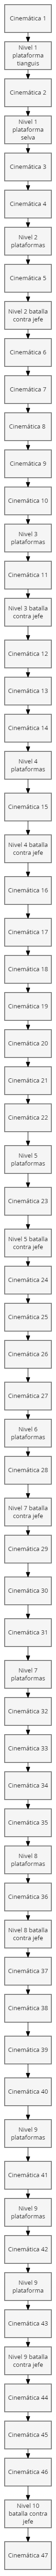
\includegraphics[width=0.1\linewidth]{Imagenes/DiagramaFlujo}
  \caption{Progreso del juego}
  \label{fig:ProgJuego}
\end{figure} 

\section{Personajes}

\subsection{Nombre: Malinalli Tenépal.} \label{per.malinalli}
	\subsubsection{Descripción:}
Joven de quince años de origen mexica. Malinalli tiene el cabello negro y largo por debajo de la cintura, acostumbra a llevarlo suelto, usando solo una peineta con forma de flor para sujetarlo del lado izquierdo de la cabeza. Sus ojos son de color café obscuro y su piel es morena. Viste un top y un short color manta. Su calzado es propio del que usaban los guerreros mexicas de alto rango, siendo del mismo color que el resto de su ropa.   
\subsubsection{Imagen}
Ver figura \ref{fig:malinnalli}
\begin{figure}
	\centering
	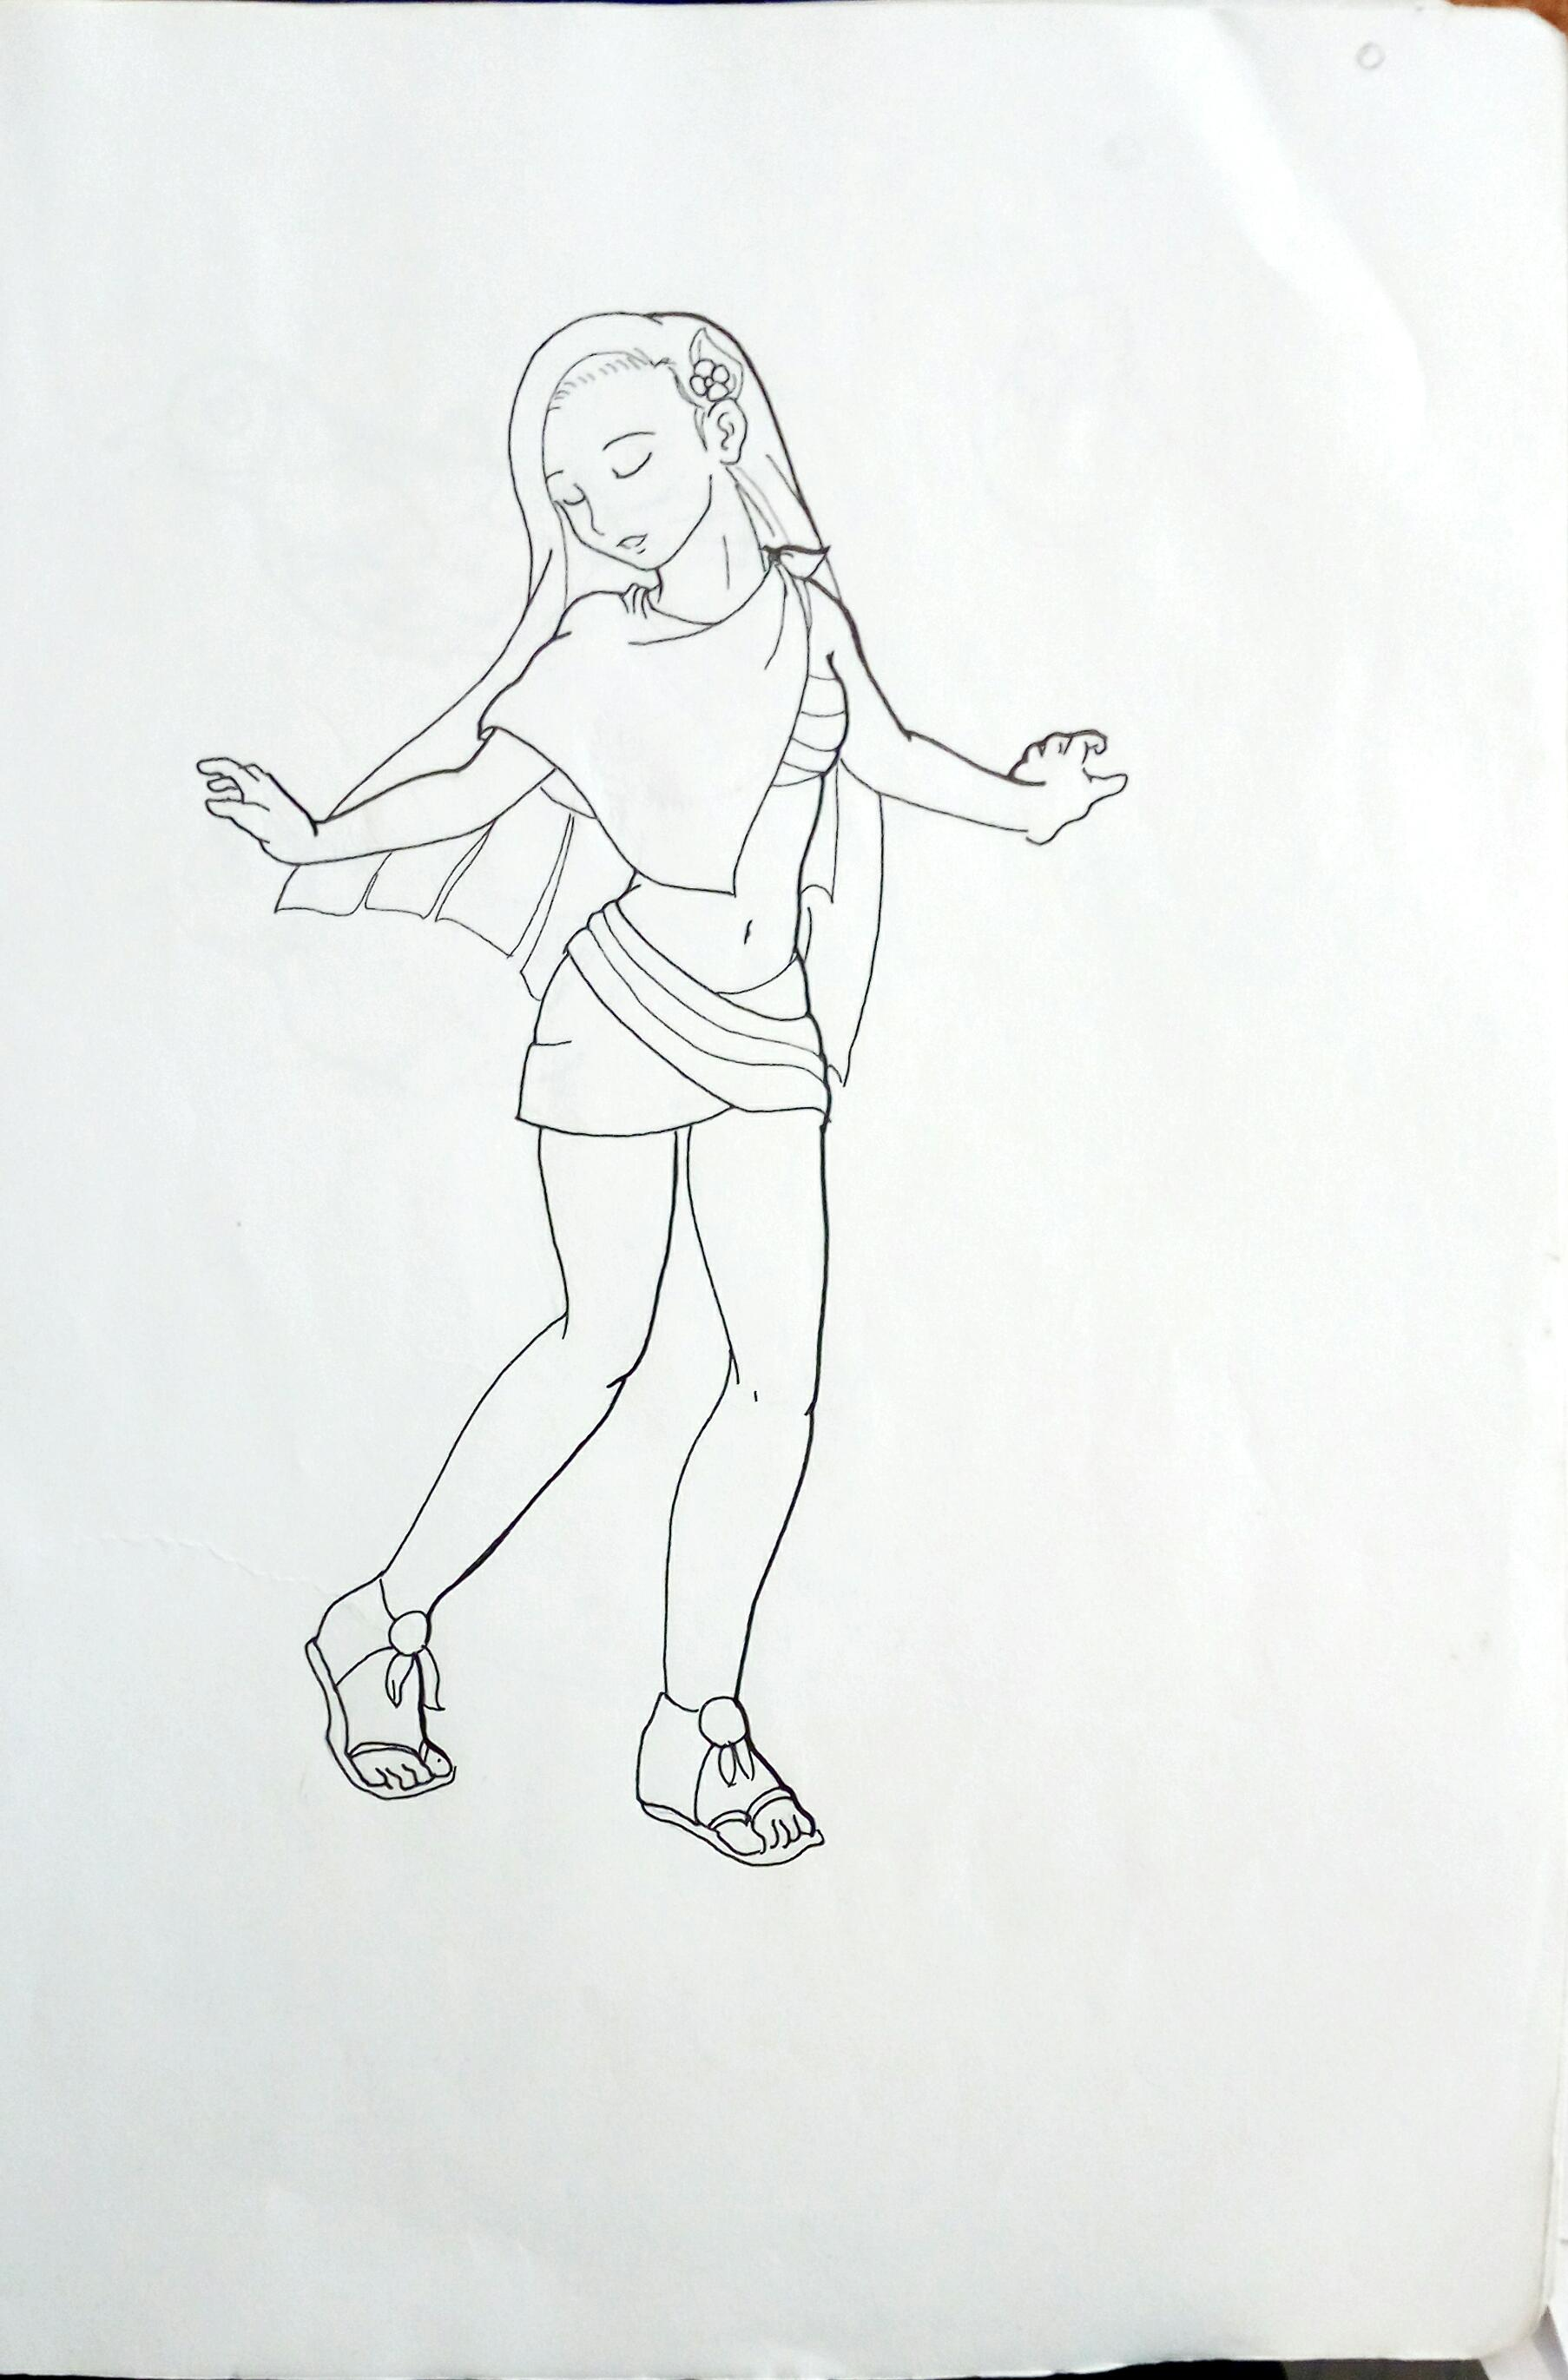
\includegraphics[height=0.2 \textheight]{Imagenes/Malinalli_Concepto}
	\caption{Malinalli.}
	\label{fig:malinalli}
\end{figure} 
\subsubsection{Concepto:}
\begin{itemize}
	\item \textbf{Historia antes del juego:}
	Hija del cacique de Oluta. Gracias a su posición social y a la educación recibida de su padre Malinalli fue capaz de aprender y de desarrollar habilidades que cualquier otra niña de su edad no habría podido al ser consideradas como propias de los hombres. Con la muerte de su padre y el segundo matrimonio de su madre, Malinalli es vendida como esclava sin que su madre hiciera algo por impedirlo. Esto causaría en Malinalli un fuerte impacto, impidiéndole a futuro poder confiar en los demás.
	\item \textbf{Historia durante el juego:}
	Los años de esclavitud logran en Malinalli una pérdida de confianza. Malinalli se percibe a si misma como débil e incapaz de hacer un cambio significativo. Desde la perspectiva de Malinalli, su papel se limita a lograr la resurrección de su padre para que él sea quien derrote al imperio y libere a su gente.
	\\
	\par 
	Al principio del juego, Malinalli se mostrará callada y medianamente abierta a mostrar sus emociones. Conforme el viaje avanza, Malinalli se irá volverá más decidida y fuerte. En un principio su motivación será revivir a su padre, pero en algún punto del juego se dará cuenta de que dicha tarea es imposible por lo que su nueva meta será destruir al imperio Mexica para unificar todos los territorios y crear el ombligo de la Luna. Cuando el viaje termine, Malinalli habrá comprendido que para cumplir sus objetivos deberá adaptarse y tener más de mil caras dependiendo de la situación.
	
	\item \textbf{Relaciones:}
	\begin{itemize}
		\item \textbf{Padre:} Es la persona más importante en la vida de Malinalli y a quien más admira.
		\item \textbf{Cimatl: } Madre de Malinalli. Malinalli guarda un fuerte odio hacia ella.
		\item \textbf{Xólotl:} En un principio no confía en Xólotl pues piensa que él la va a abandonar en cuanto deje de considerarla útil. Cuando Malinalli comprende el poder que tiene sobre el Dios y sus objetivos, su actitud hacia él cambia. Deja de ser desconfiada y se muestra más servicial y amigable. Malinalli es la única que puede aconsejar a Xólotl sobre futuras acciones y posibles aliados; sin embargo, su consejo no es producto de una amistada sino del deseo de manipular al dios para que éste haga lo que le resulta más útil a los objetivos de Malinalli. 
	\end{itemize}			  
\end{itemize}


\subsubsection{Encuentro:}
Es la protagonista del juego y es a través de ella que el jugador verá como está compuesto la dimensión divina y sus problemas. 

\subsubsection{Habilidades:}
\begin{itemize}
	\item \textbf{Disparo de tonalli:} Con ayuda de la caracola Malinalli es capaz de disparar tonalli.
	\item Malinalli posee una gran inteligencia y capacidad de planeación. Debido a sus años como esclava está en buena condición para correr y saltar.
\end{itemize} 
\subsubsection{Armas:}
\textbf{Caracola:} Esta arma con forma de cenzontle contiene el alma de uno dentro, lo que le permita generar todo tipo de sonidos. El sonido que produce se ve materializado como energía luminosa que puede atacar a los enemigos y proteger a su portador al generar una barrera. 
\subsubsection{Ítems:}
\begin{itemize}
	\item Peineta en forma de flor.
	\item Armadura espiritual.
\end{itemize}

\subsection{Nombre: Xólotl}  \label{per.xolotl}

\subsubsection{Descripción:}
En su forma de xoloitzcuintle es color verde grisáceo y un poco más grande que un xoloitzcuintle adulto normal. Porta una máscara blanca con decoraciones en la parte de los ojos y la nariz. Usa un collar con el símbolo del viento y un brazalete de oro en la pata delantera izquierda.
\\ 
\par
En su forma ajolote, es del tamaño suficiente como para que Malinalli pueda subir en el para atravesar el primer nivel del Mictlán. Al igual que en su forma xoloitzcuintle, porta una máscara blanca.
\\ 
\par
En su forma de cuervo, Xólotl mantiene el tono verde grisáceo y la mascara que lo caracteriza que lo caracteriza.
\\ 
\par
En su forma humana, adopta la apariencia de la persona en quien más confié Malinalli para que ella se familiarice con él; por tal motivo su rostro es idéntico al del padre de Malinalli. Porta ropas propias de un guerrero con los colores característicos del Dios (verde grisáceo y rojo). 
\subsubsection{Status:}
Personaje no jugable.
Xólotl le explicara al jugador el funcionamiento del juego ya sea diciéndole cómo funcionan determinados ítems, que es lo que debe o no debe de hacer en cada nivel del inframundo, la historia de algunos enemigos y darle contexto al jugador sobre el estado actual de los dioses. Xólotl también será un compañero de apoyo en algunos combates o niveles.
\subsubsection{Imagen}
Ver figura \ref{fig:xolotl}
\begin{figure}
	\centering
	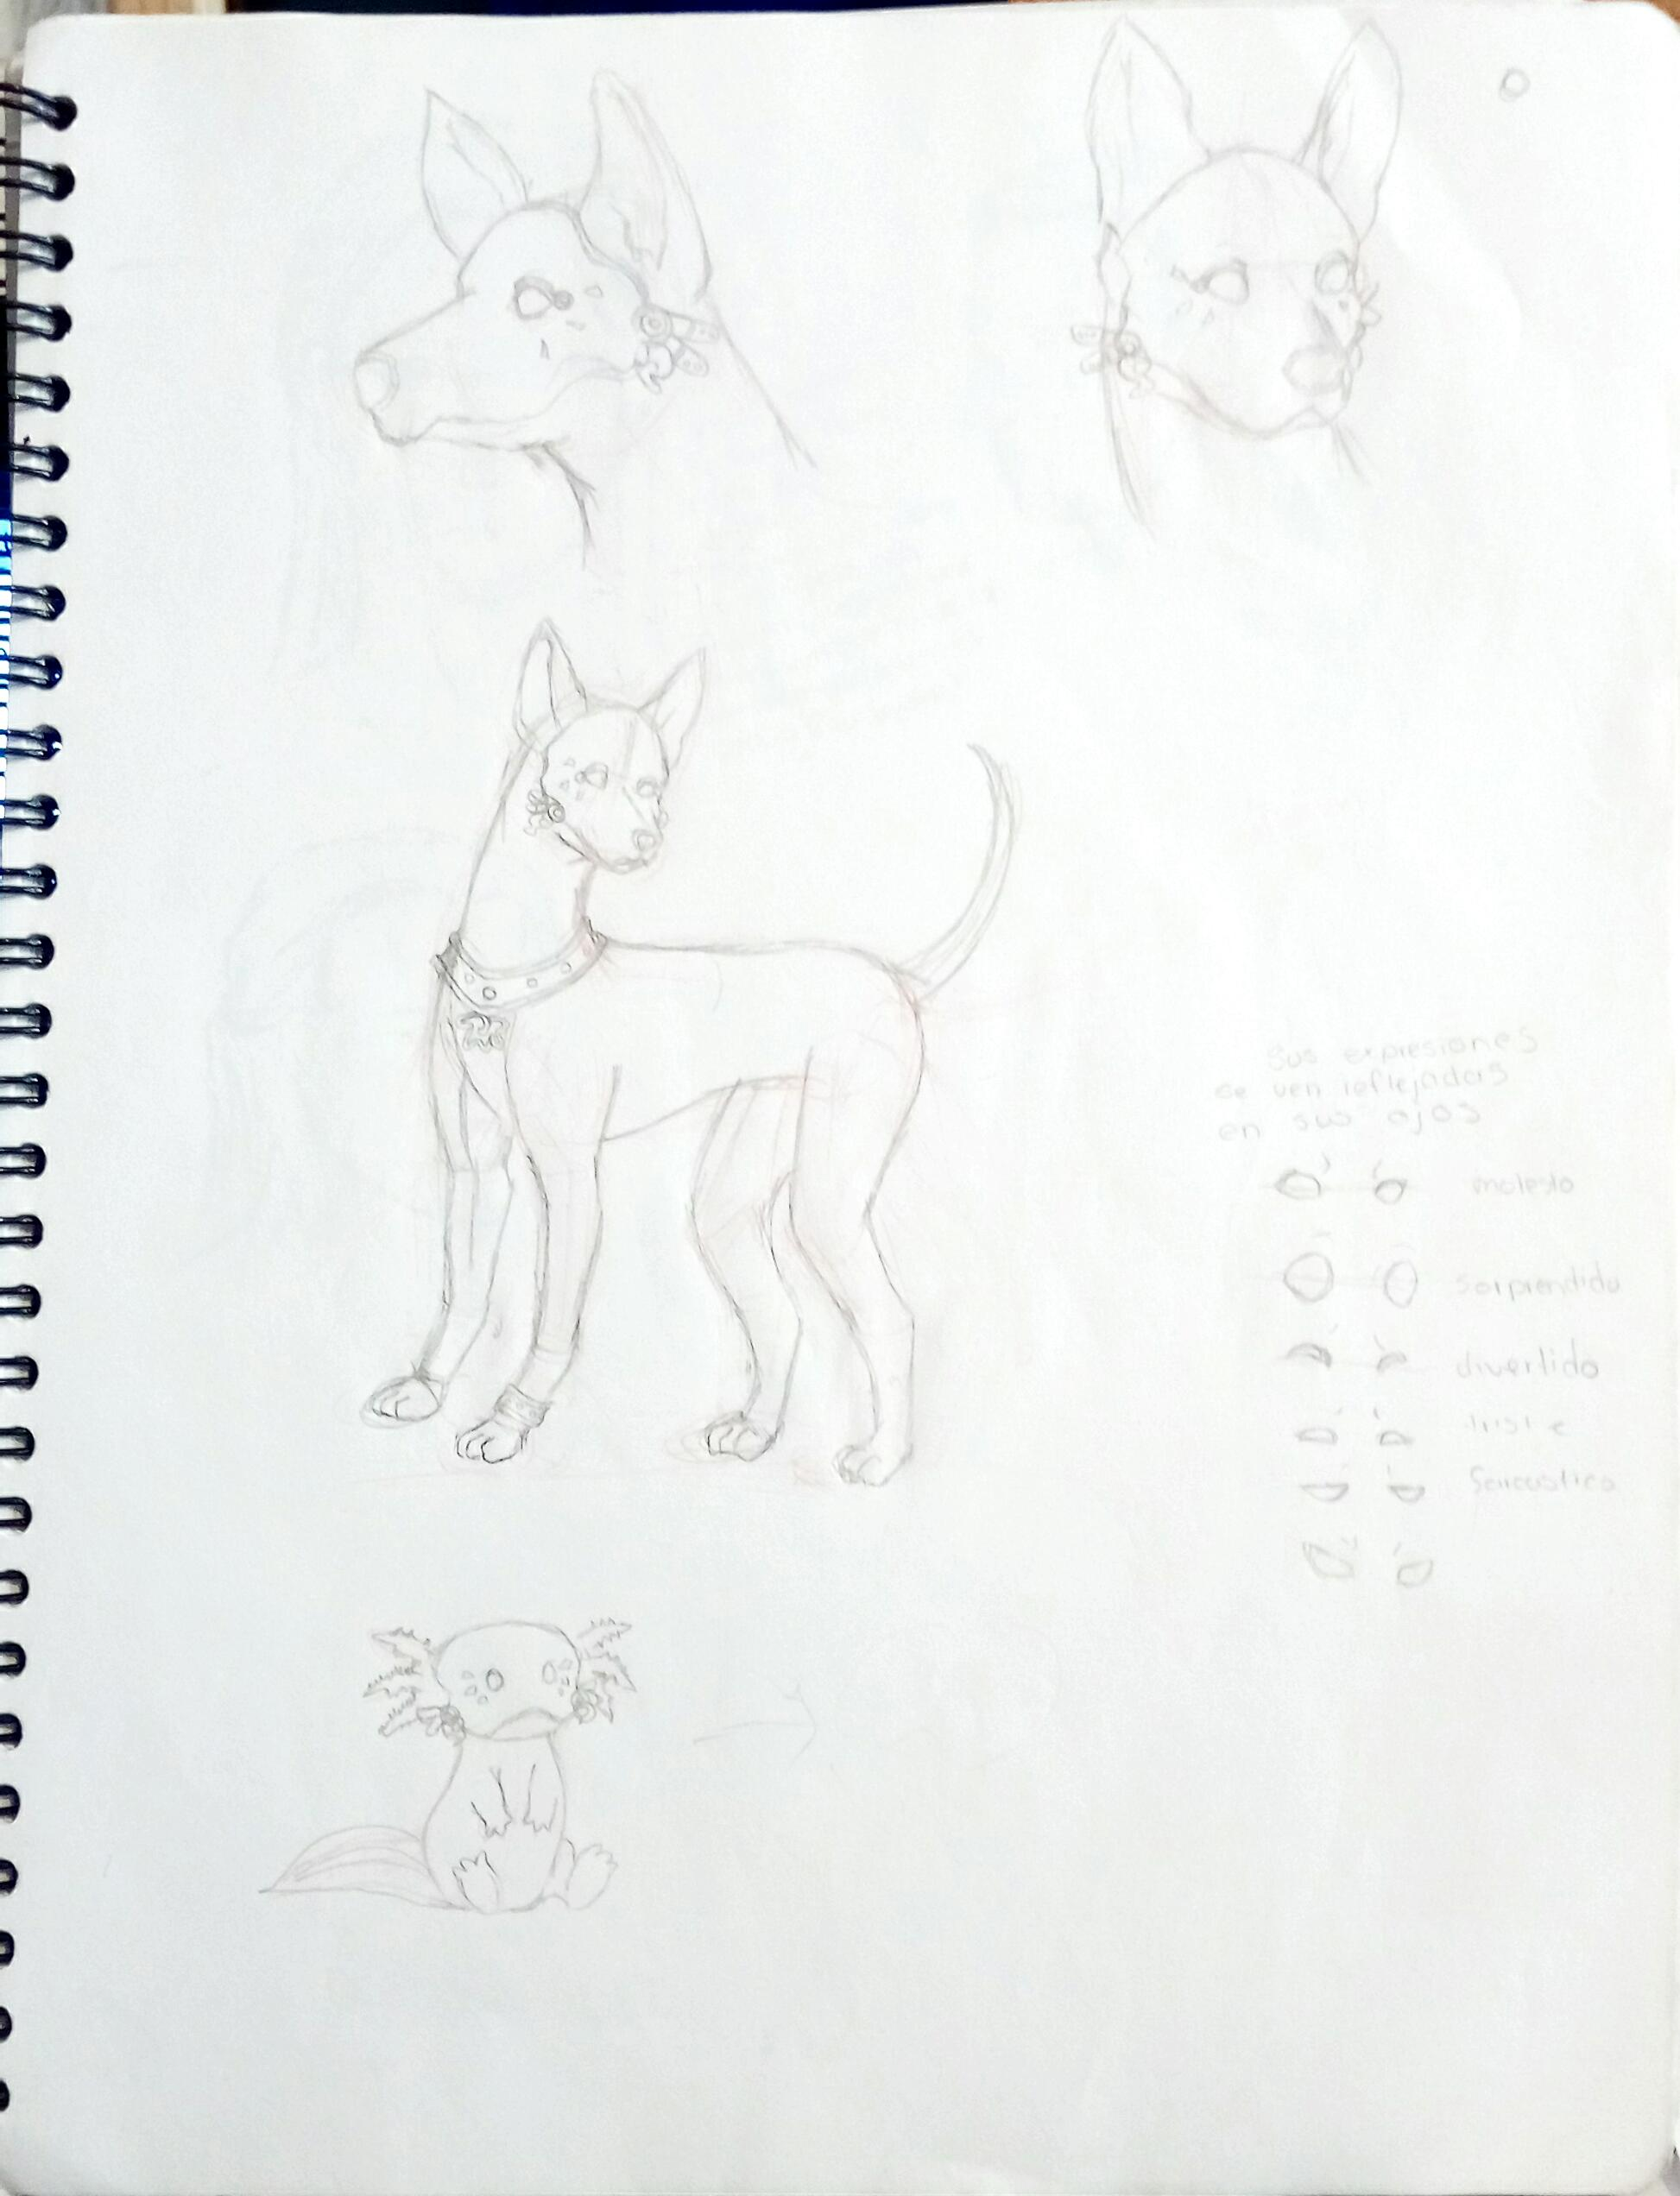
\includegraphics[height=0.2 \textheight]{Imagenes/XolotlConcepto}
	\caption{Xolotl.}
	\label{fig:xolotl}
\end{figure} 
\subsubsection{Concepto:}
\begin{itemize}
	\item \textbf{Historia antes del juego:}
	Dios gemelo de Quetzalcóatl. De carácter simpático y bromista, su personalidad le valió el cariño de muchos dioses, sin embrago muy dentro de sí Xólotl era egoísta y poseía un gran miedo a perder el reconocimiento de los demás y a la muerte. Antes de la creación del quinto sol tenía una posición privilegiada en la jerarquía divina, misma que perdió cuando se rebeló contra Quetzalcóatl y Tezcatlipoca. Su rebelión no solo le costó cargó sino también lo condenó a vagar por la tierra de los mortales en el exilio.
	\\ 
	\par 
	Durante el tiempo que vago en la tierra de los mortales, Xólotl observo el ascenso de la ciudad de Tula  y su posterior caída causada por la rivalidad existente entre Quetzalcóatl y Tezcatlipoca. Este hecho lo llevaría a tomar la decisión de destruir a ambos Dioses e instaurar un nuevo orden en el mundo espiritual; ya que, desde el punto de vista de Xólotl, los conflictos entre Quetzalcóatl y Tezcatlipoca terminarían causando la ruina de todas las civilizaciones, tal como había pasado con Tula y esto podría ocasionar la muerte de todos los dioses. Su causa no es motivada por un desinteresado deseo por el bien común sino por su profundo miedo a la muerte. 
	\item \textbf{Historia durante el juego:}
	Xólotl lucha constantemente por ocultar sus miedos e inseguridades tras su fachada sarcástica y divertida. Su constante deseo de reconocimiento lo hace buscar justificar todas su acciones bajo mascaras de heroísmo o de hacer lo correcto por lo que difícilmente admitirá que el motivo tras su viaje es su miedo a la muerte. 
	\item \textbf{Relaciones:}
	\begin{itemize}
		\item \textbf{Quetzalcóatl:} Hermano gemelo de Xólotl. Xólotl siente una fuerte envidia hacia él debido al nivel de aceptación que tiene Quetzalcóatl tanto entre los mortales como entre los Dioses.
		\item \textbf{Tezcatlipoca:} Xólotl le guarda un fuerte rencor a Tezcatlipoca desde que se enfrentaron en Tula. Para Xólotl, Tezcatlipoca no es nada más que un petulante malicioso. 
		\item \textbf{Malinalli:} Compañera de Xólotl en su viaje por el Mictlán. Después de tomar la decisión de instaurar un nuevo orden, Xólotl decide buscar un compañero que actué por él en su lucha contra los Dioses, esto debido a que si algo salía mal el podría huir. Al principio Xolotl busca guerreros, hechiceros y sacerdotes, no obstante, desiste al darse cuenta de que ninguno de ellos lucharía a su lado para destruir a los Dioses. Xólotl elige a Malinalli ya que la considera como un reflejo de él mismo al tener historias parecidas.
	\end{itemize}			  
\end{itemize}


\subsubsection{Encuentro:}
El jugador lo ve por primera vez en la cinemática 1 en su forma de humana. Siendo su primer encuentro con Malinalli en el primer nivel, en donde en su forma de xoloitzcuintle hace que Malinalli lo siga para probarle que es digna de su poder. 

\subsubsection{Habilidades:}
Sus habilidades están son de carácter mágico. Puede cambiar de forma como le plazca.
\subsubsection{Armas:}
\textbf{Atardecer de venus:} báculo que permite amplificar la magia de quien lo porta. Xólotl solamente puede utilizarlo en su forma humana.
\subsubsection{Ítems:}
Sin ítems.

\subsubsection{Personaje No-Jugable}
Xólotl le explicara al jugador el funcionamiento del juego ya sea diciéndole cómo funcionan determinados ítems, que es lo que debe o no debe de hacer en cada nivel del inframundo, la historia de algunos enemigos y darle contexto al jugador sobre el estado actual de los dioses. Xólotl también será un compañero de apoyo en algunos combates o niveles.

\subsection{Nombre: Xochitónal}  \label{per.xochitonal}

\subsubsection{Descripción:}
Iguana gigante de color rojo grisáceo y ojos naranjas. Porta una armadura de huesos que protege su espina dorsal, y su rostro.
\\
\par
Xochitonal normalmente es de actitud calmada y carácter amable. Disfruta de nadar y evita en la medida de lo posible salir del agua, ya que es el lugar en donde se siente más seguro.  
\subsubsection{Status:}
Personaje no jugable.
Jefe-enemigo del primer nivel.
\subsubsection{Imagen}
\subsubsection{Concepto:}
\begin{itemize}
	\item \textbf{Historia antes del juego:}
	Xochitónal es el único guardián del Mictlán que no es un Dios. Creado por Mictlantecuhtli durante la era posterior al Quinto Sol. Xochitónal tiene como deber proteger la entrada al Mictlán, motivo por el que patruya el rio Apanohuacalhuia y debora las almas de todos aquellos que no sean dignos de la ayuda de un Xoloitzcuintle o que por diversos motivos no lograron pasar.
	\item \textbf{Historia durante el juego:}
	Xochitónal es el primer jefe a derrotar por lo que su rol no tiene mucho peso sobre la historia.
	\item \textbf{Relaciones:}
	\begin{itemize}
		\item \textbf{Mictlantecuhtli:} Es su creador. Xochitónal guarda un profundo respeto por él y procura a odecerlo en la medida que sus habilidades se lo permitan. Su lealtad hacia él es tanta que Xochitónal esta dispuesto a morir por su creador.
		\item \textbf{Mictecacíhuatl:} Como esposa de su creador. Xochitónal tiene una relación de absoluto respeto hacia la reina del Mictlán. 
		\item \textbf{Xólotl:} Dado que fue creado después del quinto sol, nuca pudo convivir con Xólotl por lo que su opinion hacia él se basa totalmente en lo poco que ha escuchado de los demás guardianes del inframundo.
	\end{itemize}			  
\end{itemize} 
\subsubsection{Encuentro:}
\begin{itemize}
	\item Su primera aparición es en la cinemática 5. 
	\item El jugador se enfrenta a él como jefe del segundo nivel del juego.
\end{itemize}
\subsubsection{Habilidades:}
Al ser el guardián del río  Apanohuacalhuia, las habilidades de Xochitónal son sobre el control del agua:
\begin{itemize}
	\item \textbf{Zambullida:} Zochitónal se sumerge en el río, dejando solo en la superficie parte de su espalda; procediendo a nadar a gran velocidad de un lado a otro para embestir a sus enemigos.  
	\item \textbf{Burbujas:} Zochitónal dispara burbujas que seguirán al jugador por un tiempo. 
\end{itemize}
\subsubsection{Armas:}
Sin armas.
\subsubsection{Ítems:}
Sin ítems.

\subsection{Nombre: Tepeyóllotl}  \label{per.tepeyollotl}
\subsubsection{Descripción:}    
Dios jaguar, es de un tamaño ligeramente mayor al de un jaguar normal. Porta joyería fina para marcar su posición en la jerarquía divina. Usa un collar de oro con extensiones que protegen su espalda. Porta un arete de esmeralda en la oreja izquierda y un brazalete de oro en la pata izquierda. Su coraza de piedra cubre todo su cuerpo salvo por sus ojos. La coraza muestra pequeños detalles de como es Tepeyóllotl, omitiendo los detalles de su joyería y adornos, mostrando con pocas lineas detalles como su nariz y las lineas del hocico.
\\
\par
Tepeyóllotl es un personaje astuto y observador, solo observando a los demás puede darse cuenta de las verdaderas intensiones de alguien pero se guardará sus descubrimientos para él mismo a no ser que pueda obtener alguna ventaja por comunicárselo a alguien. Como cualquier felino, es orgulloso, una vez herido su orgullo es difícil recuperar su amistad. \subsubsection{Status:}
Personaje no jugable.
Jefe del tercer nivel del juego y nuevamente jefe del octavo nivel del juego.
\subsubsection{Imagen}
Ver figura \ref{fig:tepeyollotl}
\begin{figure}
	\centering
	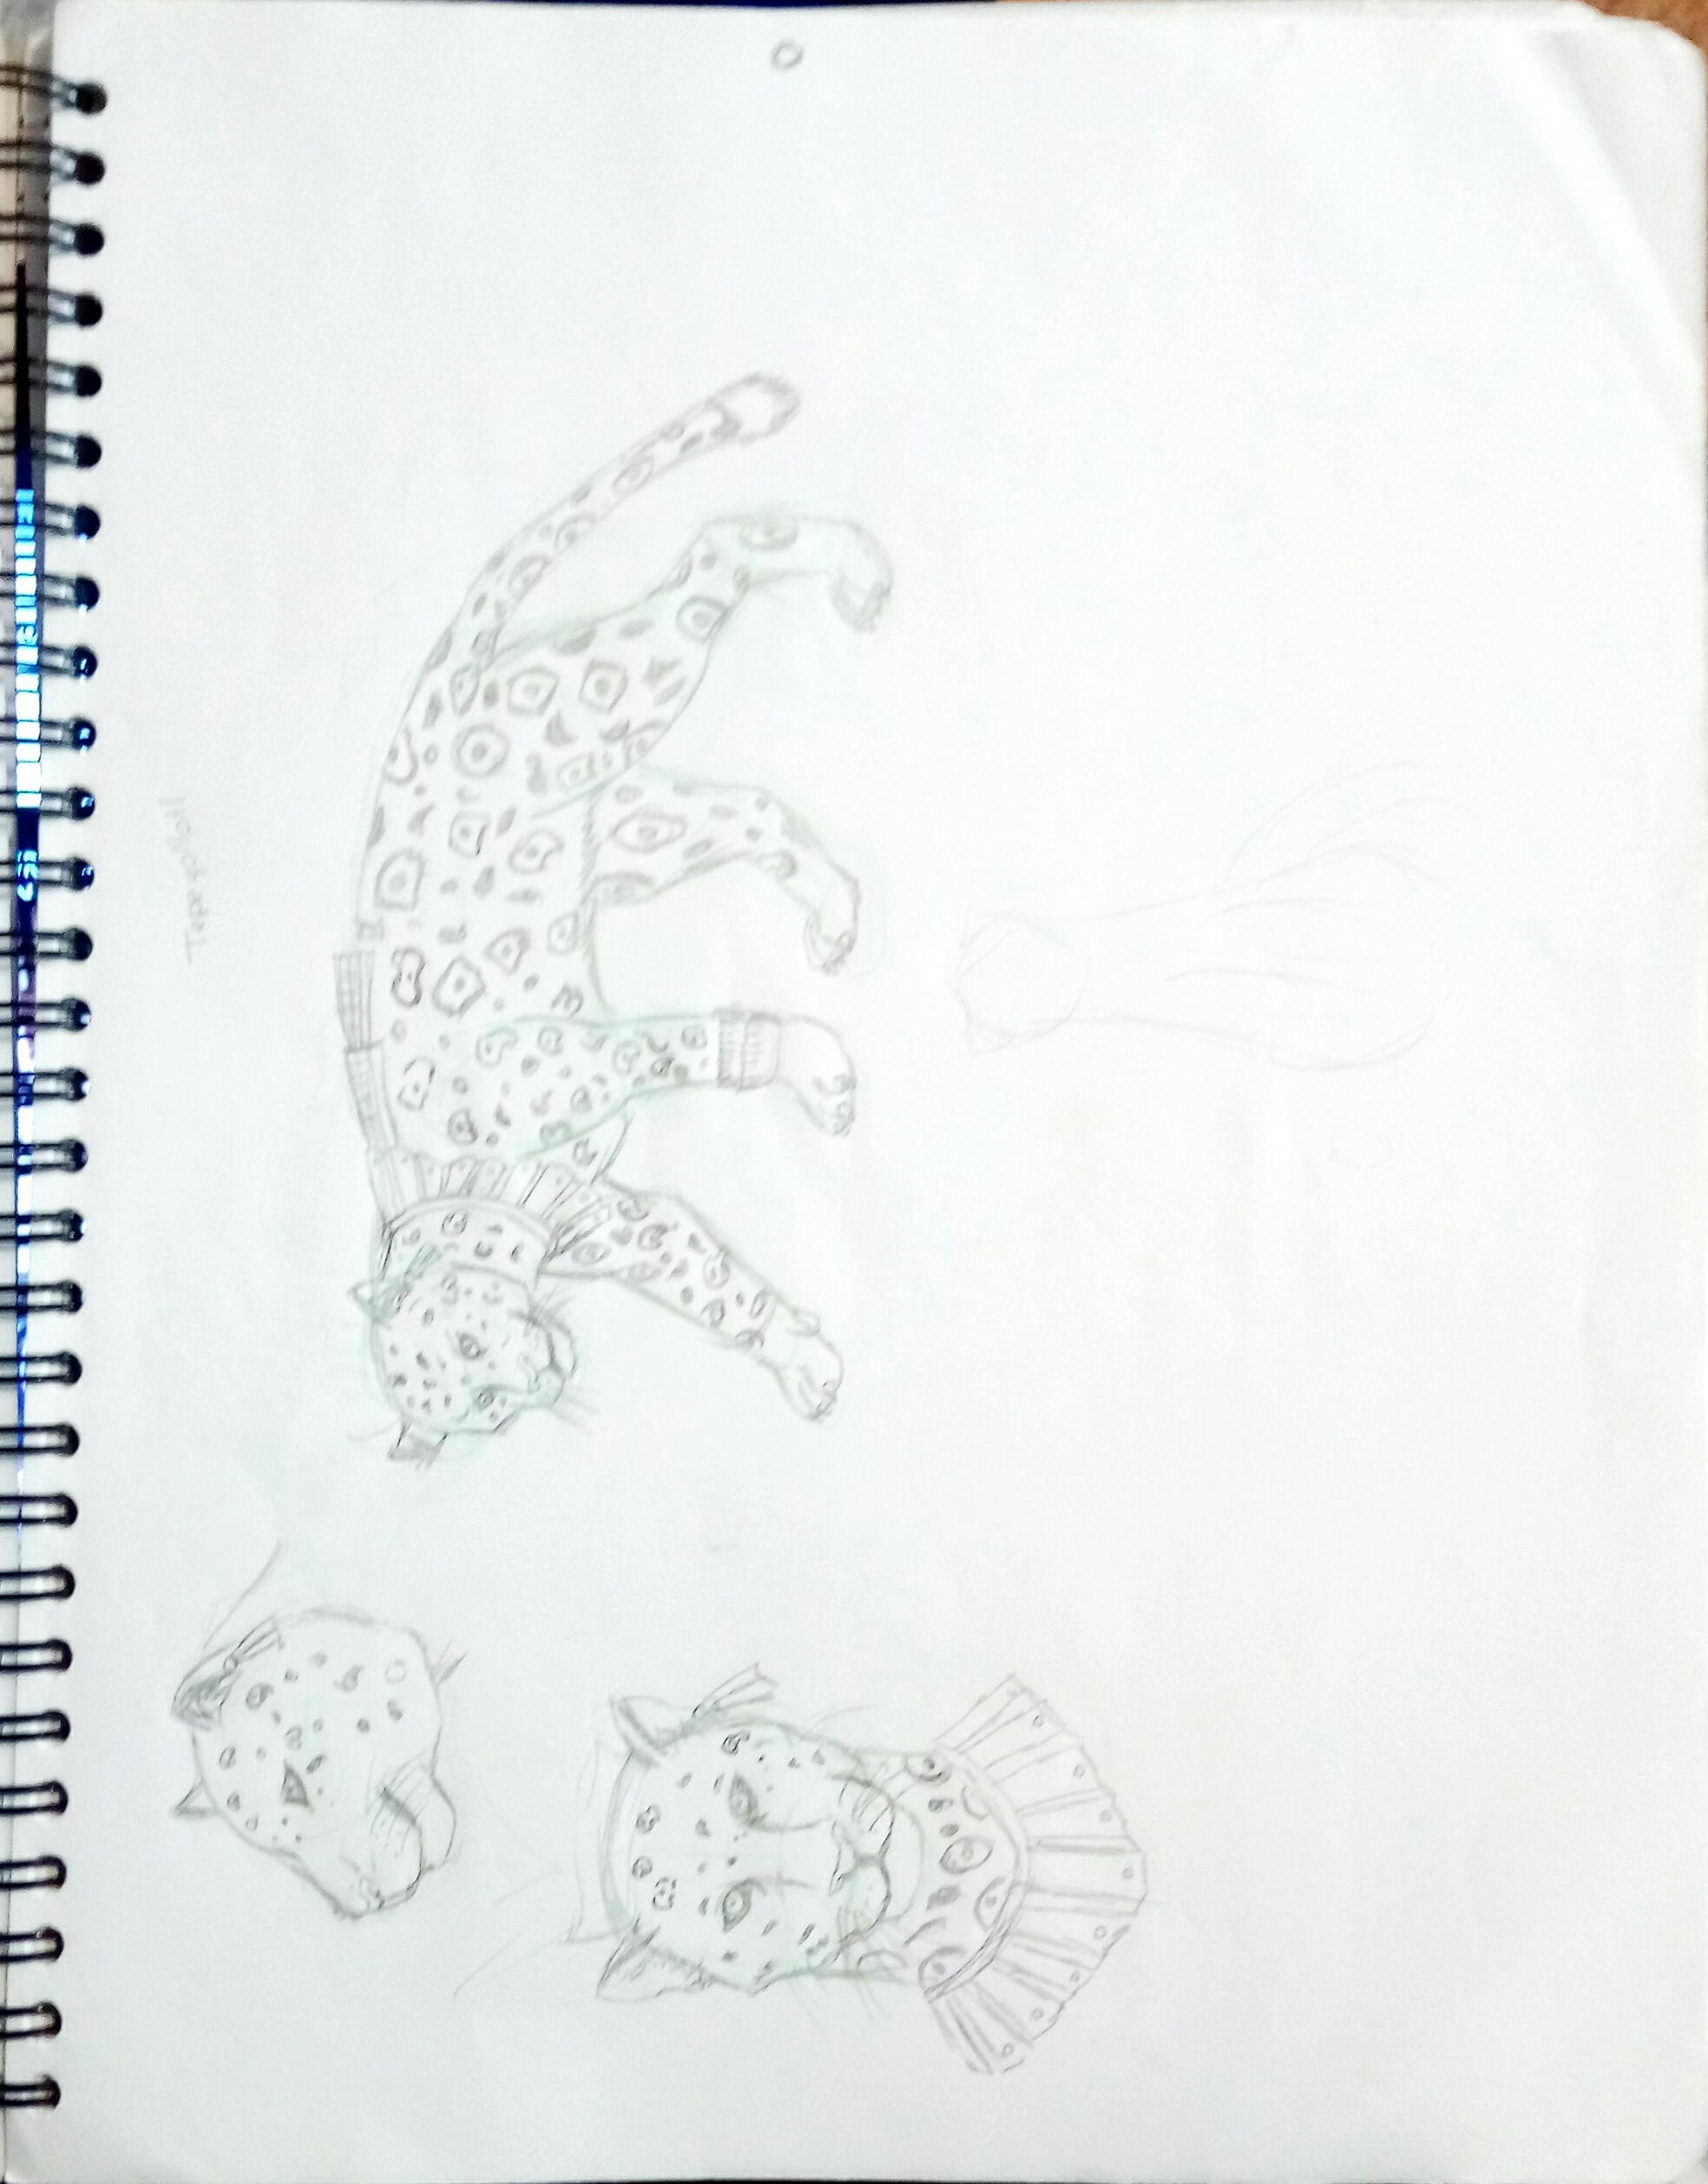
\includegraphics[height=0.2 \textheight]{Imagenes/TepeyollotlDisenio}
	\caption{Tepeyollotl.}
	\label{fig:tepeyollotl}
\end{figure} 
\subsubsection{Concepto:}
\begin{itemize}
	\item \textbf{Historia antes del juego:}
	Antes de la era del quinto Sol, Tepeyóllotl gozaba de una posición medianamente favorable dentro de la jerarquía divina. Su papel se limitaba a cumplir su rol como dios de las montañas. 
	\\
	\par
	La era del quito sol trajo consigo no solo una reestructuración de la jerarquía divina sino a su vez desato un gran numero de insurrecciones por parte de diferentes Dioses que no estaban dispuestos a abandonar sus privilegios tan fácilmente. Una vez restaurado el orden, los dioses gobernantes de los trece cielos, temerosos de futuras rebeliones, designan diferentes dioses para garantizar el orden. Por ordenes de Tezcatlipoca y por su amistad con éste, Tepeyóllotl es designado como guardian del Mictlán con el objetivo de vigilar a los demás dioses e informar a Tezcatlipoca sobre cualquier irregularidad o peligro. Su rol en el Mictlán, hace que Tepeyóllotl sea el blanco de cualquier invasor que desee conquistar el Mictlán, Tepeyollotl esta consciente de esto y por tal motivo no teme seguir sus propias reglas y alejarse de su juramento como guardián del Mictlán.   
	\item \textbf{Historia durante el juego:}
	Cuando Malinalli y Xólotl llegan al Tepeme Monamictlán, Tepeyóllotl se prepara para hacerle frente a los invasores sin saber de quienes se trataban. Al descubrir que se trataba de Xólotl, Tepeyóllotl no toma enserio la amenaza. Una vez derrotado, Tepeyóllotl consigue escapar al Teyollocualóyan con la intensión de avisarle a Tezcatlipoca sobre lo que estaba ocurriendo en el Mictlán. Sin embargo, Tepeyóllotl abandona la idea de informarle a Tezcatlipoca, al percatarse del avance de Malinalli. Es entonces que Tepeyóllotl empieza a sentir algo peligroso y obscuro creciendo dentro de ella, lo que lo lleva a concluir que Malinalli tiene otros planes además de ayudar a Xólotl.
	\\
	\par
	Con cada Dios que Malinalli va derrotando, el sentimiento de incertidumbre crece en Tepeyóllotl. Es con la caída de Tlazoltéolt que Tepeyóllotl acepta que el Mictlán esta perdido, por lo que se ve en el dilema de huir del Mictlan para advertirle personalmente a Tezcatlipoca o quedarse y tratar de averiguar más sobre Malinalli con la esperanza de ponerla en contra de Xólotl. Comprendiendo los riesgos ante la posibilidad de fallo, Tepeyóllotl manda a llamar a Mictecacíhuatl para comunicarle sus pocos descubrimientos. Hecho esto, se sienta a esperar la llegada de Malinalli y Xólotl. Sus intentos por controlar a Malinalli fallan y tal como lo había previsto el mismo Tepeyóllotl: lo único que encuentra al final de la batalla es la derrota.  
	\item \textbf{Relaciones:}
	\begin{itemize}
		\item \textbf{Tezcatlipoca:} Amigo de Tepeyóllotl. Es su jefe directo en la jerarquía divina, siendo al único al que debe de rendir cuentas sin excusas. 
		\item \textbf{Mictecacíhuatl:} Tepeyóllotl siente una admiración sincera por ella, siendo la única con quien habla en el Mictlán. Tepeyóllotl considera que  Mictecacíhuatl debería ser la novena guardiana del  Mictlán y no Mictlantecuhtli.
		\item \textbf{Mictlantecuhtli:} Desde el punto de vista de Tepeyóllotl,  Mictlantecuhtli es un líder ineficiente y de poca visión por lo que comúnmente tiene roces con él.
		\item \textbf{Xólotl:} Percibido como un niño malcriado y emberrinchado, Tepeyóllotl no tiene en buena estima a Xólotl.
		\item \textbf{Malinalli:} Considerada como el verdaero peligro para la jerarquía divina. Tepeyóllotl no se siente comodo al lado de ella pues algo le dice que la presencia de Malinalli esta ligada a la caída de todos los Dioses.
	\end{itemize}                     
\end{itemize}
\subsubsection{Encuentro:}
\begin{itemize}
	\item Su primera aparición es en la cinemática 9. 
	\item El jugador se enfrenta a él como jefe del tercer nivel del juego.
\end{itemize}

\subsubsection{Habilidades:}
\begin{itemize}

        \item \textbf{Coraza:} Esta habilidad permite crear una coraza de piedra protegiendo a su portador de ataques enemigos sacrificando velocidad de movimiento.   
        \item \textbf{Impacto:} Realiza un salto, provocando al aterrizaje una onda de piedras en el suelo.
        \item \textbf{Luvia de rocas:} Con un poderoso rugido provoca una avalancha de rocas. 
	  \item \textbf{Rugido aturdidor:} Poderoso rugido provoca una de continuo echo que inmoviliza a al enemigo, Tepeyóllotl solo puede usar esta habilidad cuando no usa la coraza. 
\end{itemize}
\subsubsection{Armas:}
Sin armas.
\subsubsection{Ítems:}
Sin ítem


\subsection{Nombre: Itzpápalotl}  \label{per.itzpapalotl}
\subsubsection{Descripción:}
Diosa de altura media y complexión delgada. De piel blanca y ojos negros. Su larga cabellera negra va arreglada en un par de trenzas. Maquilla su cara con pintura de guerra negra. Su vestimenta es el de una guerrera, con algunas variantes del uniforme militar mexica para permitirle mayor agilidad y capacidad de vuelo.  Tiene un par de alas de mariposa hechas de obsidiana que le permiten volar y realizar ataques poderosos.    

Itzpápalotl es una diosa de actitud activa, es directa y no teme decir lo que piensa pero mide sus palabras con quienes resulten más sensibles a las palabras. Itzpápalotl toma su deber con seriedad. Es una mujer segura, con una gran fuerza de voluntad e independiente. Desafortunadamente, después de la guerra contra los Dioses del Norte, Itzpápalotl desarrollo síndrome de estrés postraumático, por lo que se le dificulta luchar; siendo Itztlacoliuhqui  el único capaz de calmarla cuando tiene episodios de crisis.
\subsubsection{Status:}
Jefe enemigo del cuarto nivel del juego.
\subsubsection{Imagen}
Ver figura \ref{fig:itzpapalotl}
\begin{figure}
	\centering
	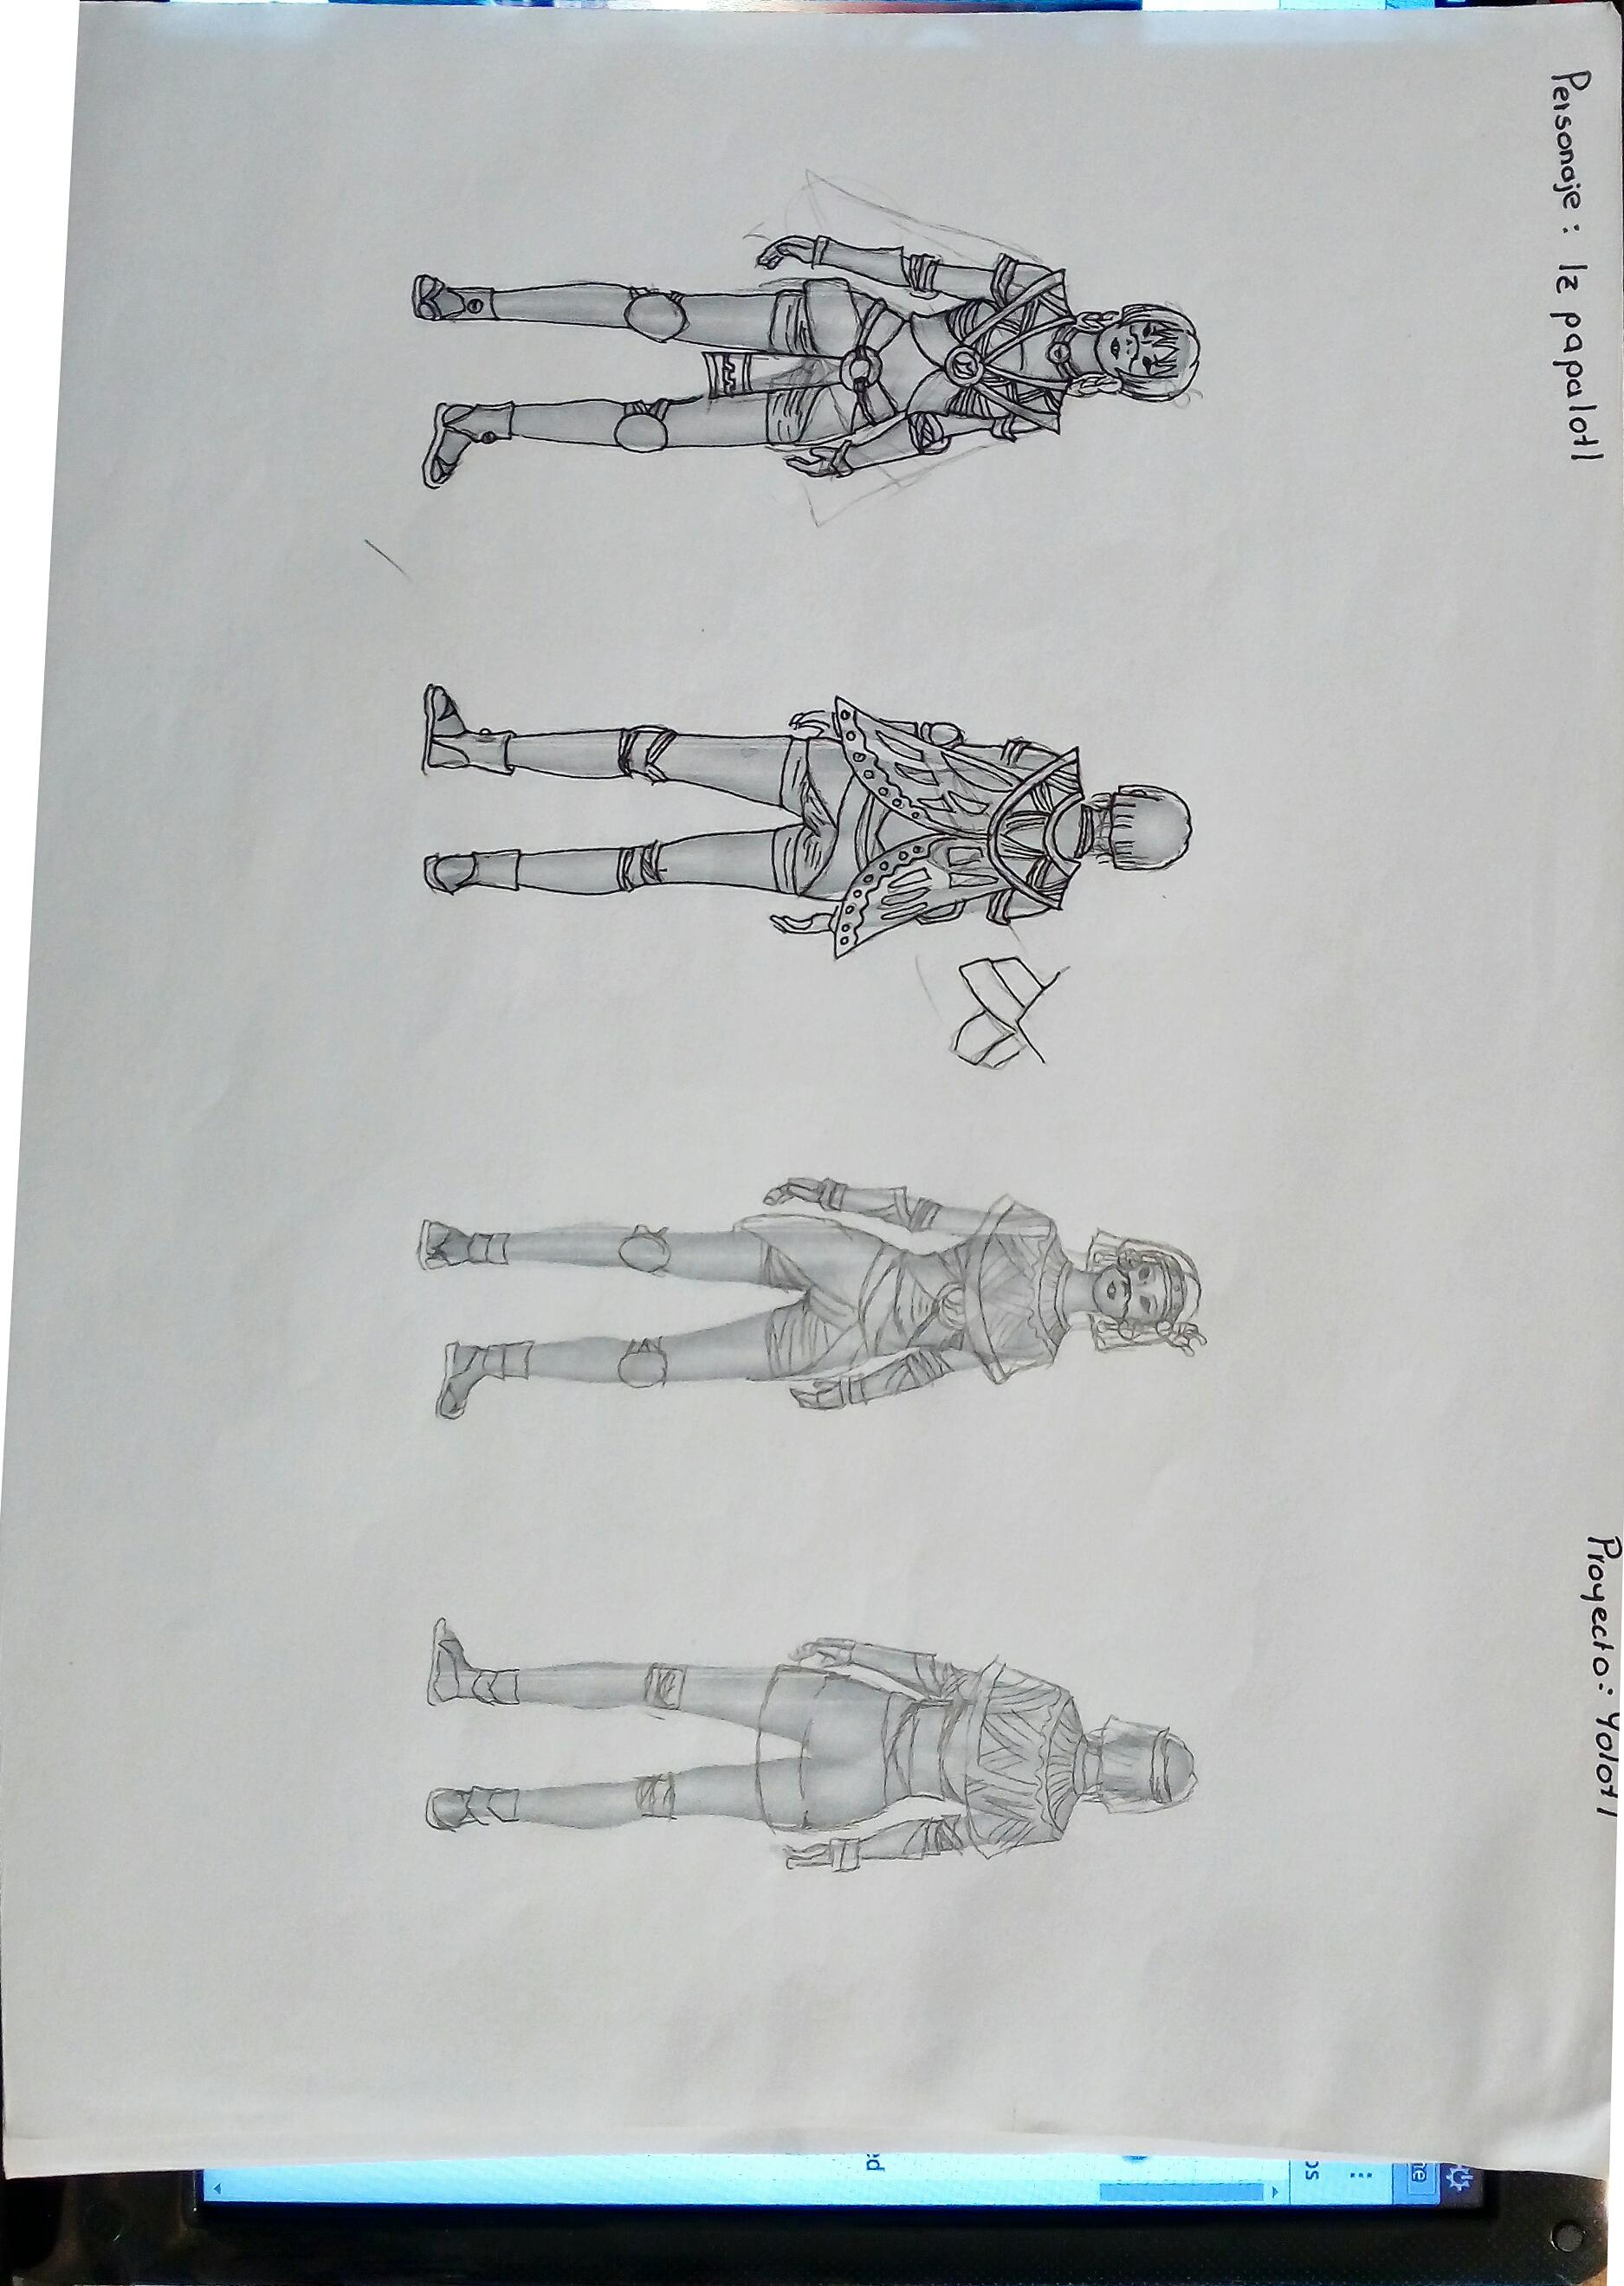
\includegraphics[height=0.2 \textheight]{Imagenes/Itzpapalotl}
	\caption{Itzpapalotl.}
	\label{fig:itzpapalotl}
\end{figure} 
\subsubsection{Concepto:}
\begin{itemize}
	\item \textbf{Historia antes del juego:}
	Itzpápalotl es una de las diosas de mayor antigüedad, siendo la primera en no adoptar un rol dedicado al hogar o a la belleza, optando por ser una diosa guerrera.
	Durante los años posteriores al quinto sol, los dioses aztecas lucharon una guerra contra los dioses del norte. En esta guerra Iztpápalotl se desempeño como una capitana de gran jerarquía logrando ganar innumerables batallas. Las victorias de Itzpápalotl no hicieron otra cosa más que llenarla de orgullo, haciéndola olvidar cualquier tipo de modestia, llegando incluso a ignorar ordenes de Dioses con un rango mayor. En una de las batallas más decisivas para la guerra, Itzpápalotl se niega a pedir refuerzos provocando que todas sus tropas sean eliminadas, rodeada por sus enemigos, Izpápalotl lucha contra quinientos dioses enemigos, derrotando a una cantidad considerable de ellos pero resultando derrotada al final. Tras su derrota los dioses enemigos deciden prenderle fuego para acabar con ella. El fuego no logra matarla, pero consigue convertir su piel en cenizas. Las heridas causadas por esa batalla lograrían hacer que Itzpápalotl se retirara del campo de batalla sin la posibilidad de volver.
	
	La derrota de Iztpápalotl traería consigo un efecto en cadena en la defensa de los Dioses aztecas culminando con la perdida de la guerra. Nuevamente instaurada la paz, Itzpápalotl siente que la derrota en la guerra es producto de sus errores. Itzpápalotl le pide entonces a Tezcatlipoca que la envie al Mictlan para que pueda enmendar sus errores al fungir como una guardiana. Siendo el Mictlán el lugar donde conoceria a su futuro esposo: Itztlacoliuhqui. 
	\item \textbf{Historia durante el juego:}
	En un principio Itzpápalotl no toma muy enserio el ataque de Xólotl al Mictlán, principalmente a que las anteriores invasiones al Mictlán habían sido detenidas únicamente con el poder de Xochitónal. Su encuentro contra Xólotl y Malinalli la toma por sorpresa ya que ella confiaba en que Tepeyóllotl sería capaz de eliminar a los invasores sin ningún problema. Es precisamente su exceso de confianza lo que define su  derrota en el enfrentamiento contra Malinalli. Cuando es derrotada por Malinalli, Itzpápalotl utiliza lo último que le queda de energía para enviarle un ultimo mensaje a Itztlacoliuhqui, mostrando que por sobre su deber estaba el amor que sentía por él.
	\item \textbf{Relaciones:}
	\begin{itemize}
		\item \textbf{Itztlacoliuhqui:} Esposo de Itzpápalotl. En él Itzpápalotl encontró la calma y el lugar seguro que necesitaba. Él es quien Itzpápalotl ama más y quien ocupa su prioridad número uno.  
		\item \textbf{Tezcatlipoca:} Le permitió a Itzpápalotl integrarse a los guardianes del Mictlán luego de que perdieran la guerra contra los Dioses del norte.   
	\end{itemize}                     
\end{itemize}

\subsubsection{Encuentro:}
\begin{itemize}
	\item Su primera aparición es en la cinemática 9. 
	\item Su primer y único encuentro con Malinalli es en el cuarto nivel del juego.
\end{itemize}
\subsubsection{Habilidades:}
\begin{itemize}
	\item \textbf{Circulo de fuego:} Itzpápalotl se eleva en el aire y se rodea a sí misma con fuego, este ataque sera usado cuando el jugador se encuentre junto a ella.
	\item \textbf{Embestida aerea:} Itzpápalotl usara este ataque cuando este lejos del jugador. Itzpápalotl saltar y en el aire se lanza contra el enemigo en diagonal.
	\item \textbf{Invisibilidad:} Esta habilidad le permite ser indetectable al ojo de dioses y humanos, permitiendole tomar una posición ventajosa en combate.
\end{itemize}
\subsubsection{Armas:}
\textbf{Matlalpapalotl} Tepoztopilli hecho de obsidiana. Arma creada por Iztpapalotl a partir de las almas de los enemigos derrotados durante la guerra contra los dioses del norte. Es un arma de gran poder, es ligera, ideal para el combate aéreo.
\subsubsection{Ítems:}
Sin ítems.



\subsection{Nombre: Mictlecayotl}  \label{per.mictlecayotl}

\subsubsection{Descripción:}
Mictlecayotl es una deidad guerrera por lo que su vestimenta está orientada a la batalla, porta una armadura ligera que le permite realizar rápidos ataques de viento, pero el costo de su rapidez es la poca defensa ante poderosos ataque que ofrece la armadura. En los antebrazos usa unos protectores que por su diseño también le permiten desgarrar a sus enemigos si estos se encuentran cerca de ella. Sus codos y sus rodillas son protegidas por unas conchas recogidas de los lagos del octavo nivel del Mictlán, estas conchas poseen la habilidad de proteger contra encantamientos que alteran el pensamiento a quien los porta. Lleva el cabello recogido en una coleta para evitar que le estorbe en combate. Su rostro esta maquillado con pintura para guerra. A manera de recordatorio de su antigua posición en la jerarquía divina porta un collar y aretes de oro. Es una mujer de estatura mediana, espalda ancha y piernas fuertes. 
\\
\par
Mictlecayotl se caracteriza por ser de actitud paciente y callada pero orgullosa. No tiene problemas para relacionarse con otros dioses. Es una persona reservada que difícilmente hablara sobre ella y sus problemas, pero está dispuesta a escuchar a los demás y a ayudarlos. Siente una gran compasión por la raza humana por lo que trata de que los difuntos encuentren la paz en su paso por su nivel del infierno por lo que no es extraño verla ayudando a quienes demuestren ser dignos.  
\\
\par
\textbf{Nota de diseño}: Su paleta de colores está basada en los códices de Ehécatl, predominando el verde en diferentes escalas y el rojo en tonalidades oscuras. 	  
\subsubsection{Status:}
Personaje no jugable.
Jefe del quinto nivel. Debe de ser derrotado para poder avanzar.
\subsubsection{Imagen}
Ver figura \ref{fig:mictlecayotl}
\begin{figure}
	\centering
	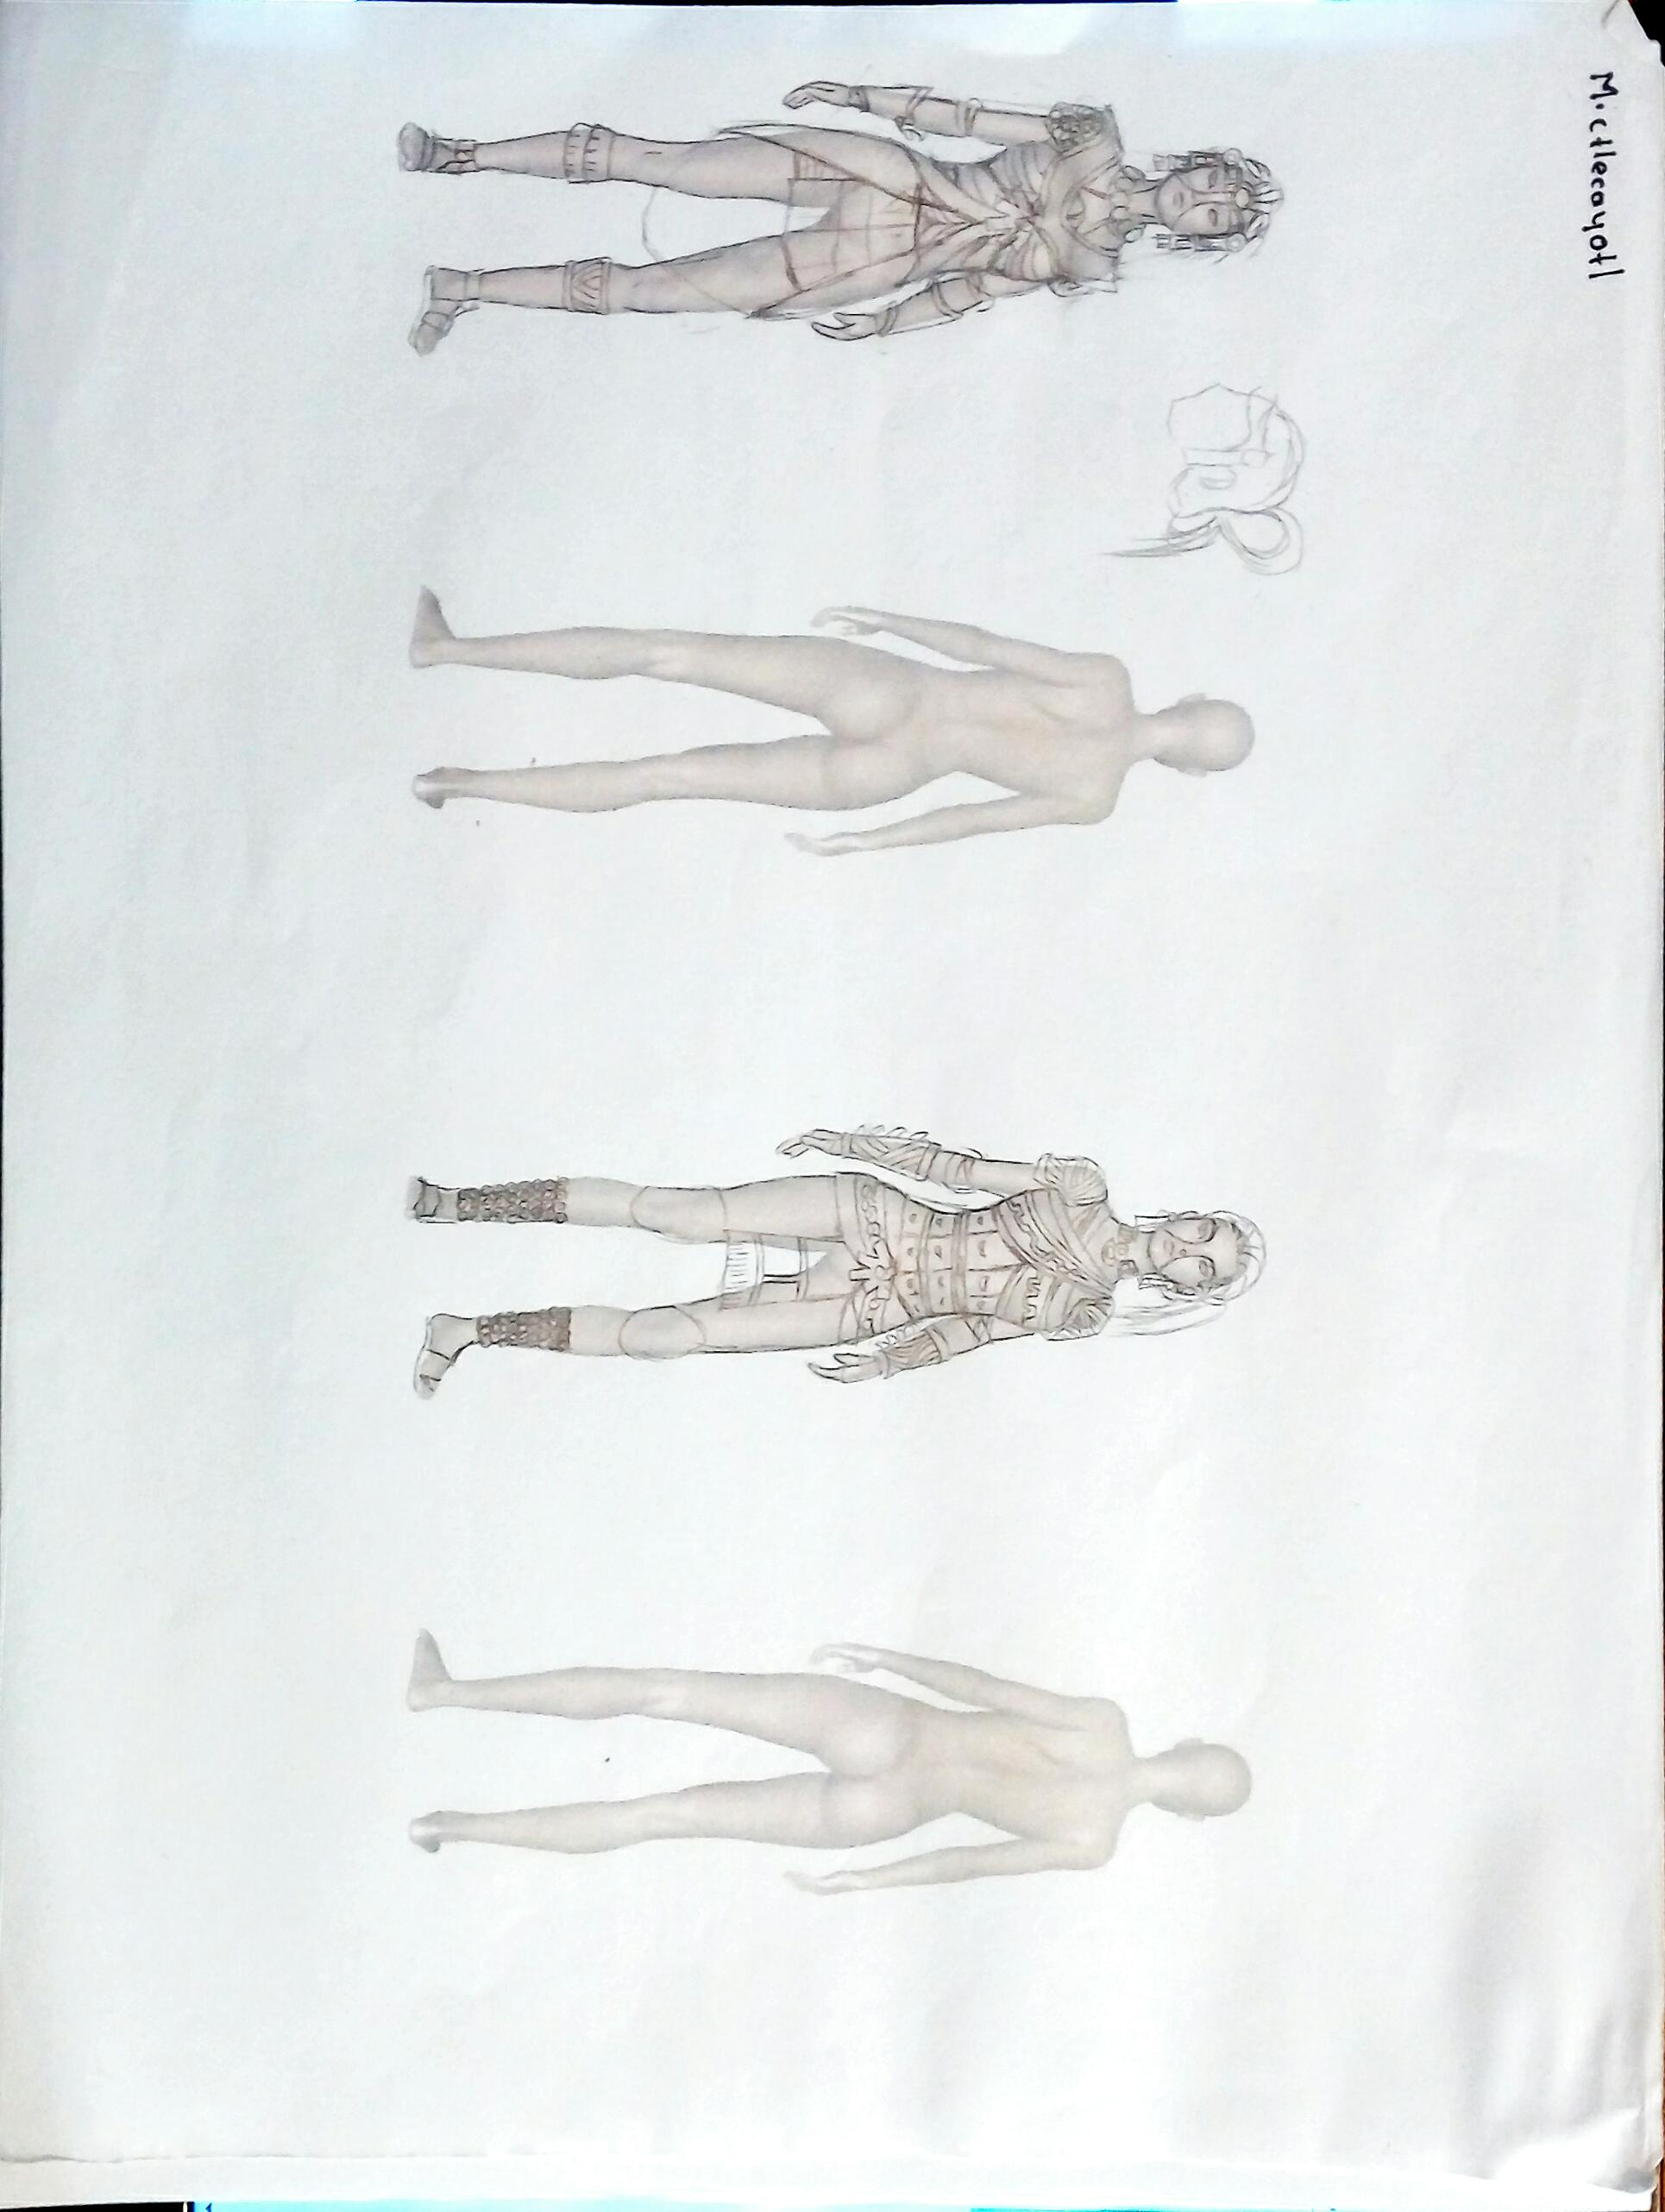
\includegraphics[height=0.2 \textheight]{Imagenes/Mictlecayotl}
	\caption{Mictlecayotl.}
	\label{fig:mictlecayotl}
\end{figure} 
\subsubsection{Concepto:}
\begin{itemize}
	\item \textbf{Historia antes del juego:}
	Mictlecayotl es la diosa del viento del norte y esposa del dios del viento Ehécatl. Durante la época anterior al exilio de Quetzalcóatl, Mictlecayotl vivía junto a su esposo en uno de los trece cielos. Luego de que su esposo se enamorara de una humana,  Mictlecayotl decide observar a los humanos para comprender que es lo que tienen de especiales, acción que la llevaría a comprender que lo que hacía bella la existencia humana era lo efímera y frágil que ésta podía ser, siendo estas características lo que impulsaba a las personas a hacer cosas extraordinarias al buscar la inmortalidad en el recuerdo popular. Observar a los humanos le permitiría además formar una amistad con Quetzalcóatl.
	\\
	\par
	Cuando Quetzalcóatl se exilia luego de la caída de Tula,  Mictlecayotl se muestra deprimida. El exilio de Quetzalcóatl trae consigo una serie de cambios en los trece cielos. De un momento a otro todos los dioses que habían simpatizado con Quetzalcóatl se ven degradados de rango y en su lugar eran puestos los simpatizantes de Tezcatlipoca. Mictlecayotl logra mantener su posición jerárquica a pesar de su amistad con Quetzalcóatl. Y al cabo de unos meses regresa a sus tareas como protectora del viento del norte. Sin embargo, una vez que descubre la verdad tras el exilio de Quetzalcóatl,  Mictlecayotl trata de asesinar a Tezcatlipoca sin éxito. Ehécatl logra convencer al dios negro de que no asesine a Mictlecayotl. Tezcatlipoca le perdona la vida a la diosa, pero determina que ella debe de sufrir un castigo por su crimen. Es así como Mictlecayotl es separada de Ehécatl y es enviada al Mictlán para fungir como guardiana del cuarto nivel del Mictlán, permitiéndole ver a Ehécatl únicamente cuando los vientos helados del norte salieran del Mictlán hacia la tierra de los mortales durante los inviernos.			
	\item \textbf{Historia durante el juego:}
	Como guardiana del cuarto nivel del Inframundo, Mictlecayotl tiene la obligación de frenar a Xolotl en su cruzada por el Mictlán. Luego de la caída de Xochitonal, Mictlantecutli ordenara a los guardianes del Mictlan proteger el inframundo y evitar a toda costa el avance de Xolotl. Mictlecayotl encontrará la muerte en su enfrentamiento con Xolotl y Malinalli pero antes de desaparecer Xolotl le contará que durante su exilio tuvo la oportunidad de encontrarse a Quetzalcóatl.
	\item \textbf{Relaciones:}
	\begin{itemize}
		\item \textbf{Xolotl:} Considerado como un traidor. La opinión de Mictlecayotl cambia cuando Xolotl le cuenta que trato de detener a Tezcatlipoca la noche que éste provoco el exilio de Quetzalcóatl. Mictlecayotl le agradece a Xolotl por tratar de ayudar a Quetzalcóatl y le pide que se encargue de Tezcatlipoca.
		\item \textbf{Ehécatl:} Esposo de Mictlecayotl. Ambos comparten una relación de respeto y apoyo mutuo. 
		\item \textbf{Quetzalcóatl:} Amigo de Mictlecayotl. Es el dios al que más admira y al único al que reconoce como digno de ser el líder de los trece cielos. Mictlecayotl espera su regreso para que traiga fin al nuevo orden que Tezcatlipoca ha instaurado.
		\item \textbf{Tezcatlipoca:} Enemigo de Mictlecayotl. Trató de matarlo en una ocasión.  
	\end{itemize}			  
\end{itemize}


\subsubsection{Encuentro:}
\begin{itemize}
	\item Su primera aparición es en la cinemática 9. 
	\item Su primer y único encuentro con Malinalli es en el quinto nivel del juego.
\end{itemize}
\subsubsection{Habilidades:}
Como diosa del viento, la principal habilidad de Mictlecayotl es manipular el viento con el que crea diferentes ataques como:
\begin{itemize}
	\item \textbf{Tornado:}  poderoso ataque que puede bajar hasta la mitad de la vida del jugador.
	\item \textbf{Ventisca:} Aire helado que puede causar una pérdida considerable de la barra de salud.
\end{itemize}

Sus habilidades de viento también le permiten desvanecerse en el aire y aparecer en una posición ventajosa para su ataque.
\subsubsection{Armas:}
\textbf{Trepa viento:} Macuahuitl creada por Mictlecayotl para canalizar su energía de viento y generar poderoso ataques.
\subsubsection{Ítems:}
Sin ítems.

\subsection{Nombre: Tlazoltéotl}  \label{per.tlazolteotl}
\subsubsection{Descripción: }  
De estatura pequeña y gran belleza. De todas las guardianas del Mictlán Tlazoltéotl es quien posee mayor feminidad. Es de piel morena, cabello negro y largo a la altura de la cintura que acostumbra a llevar suelto. De pechos grandes y cadera ancha. Al igual que la mayoria de los Dioses usa joyería de oro fino. En la mano derecha porta una delicada pulsera y en la mano izquierda usa un brazalete con labrados que le cubre casi todo el antebrazo. Usa un par de aretes de jade y un collar de oro adornado con un cuerno de jade de gran tamaño. Tlazoltéotl acostumbra a ir descalza ya que sus movimientos son parecidos a los de una danza y de esta manera se siente mas ligera. Viste un delgado top y una falda que le tiene una ligera abertura entre las piernas, la cual le permite moverse con mayor facilidad.
\\
\par
Tlazoltéotl es de actitud risueña y juguetona pero seductora. Es consciente de la gran belleza que posee y le divierte usarla para confundir a los demás sobre sus intensiones. Disfruta de hablar a manera de acertijo. Posee una mente abierta y dificilmente se sorprende, acostumbra a aburrirse de las cosas rapidamente por lo que le cuetas trabajo enfocarse en sus tareas; sin embargo, desempeña sus deberes con eficiencia una vez que se enfoca.    
\subsubsection{Status:}
Personaje no jugable.
Es el jefe enemigo del secto nivel del juego.
\subsubsection{Imagen}
Ver figura \ref{fig:tlazolteotl}
\begin{figure}
	\centering
	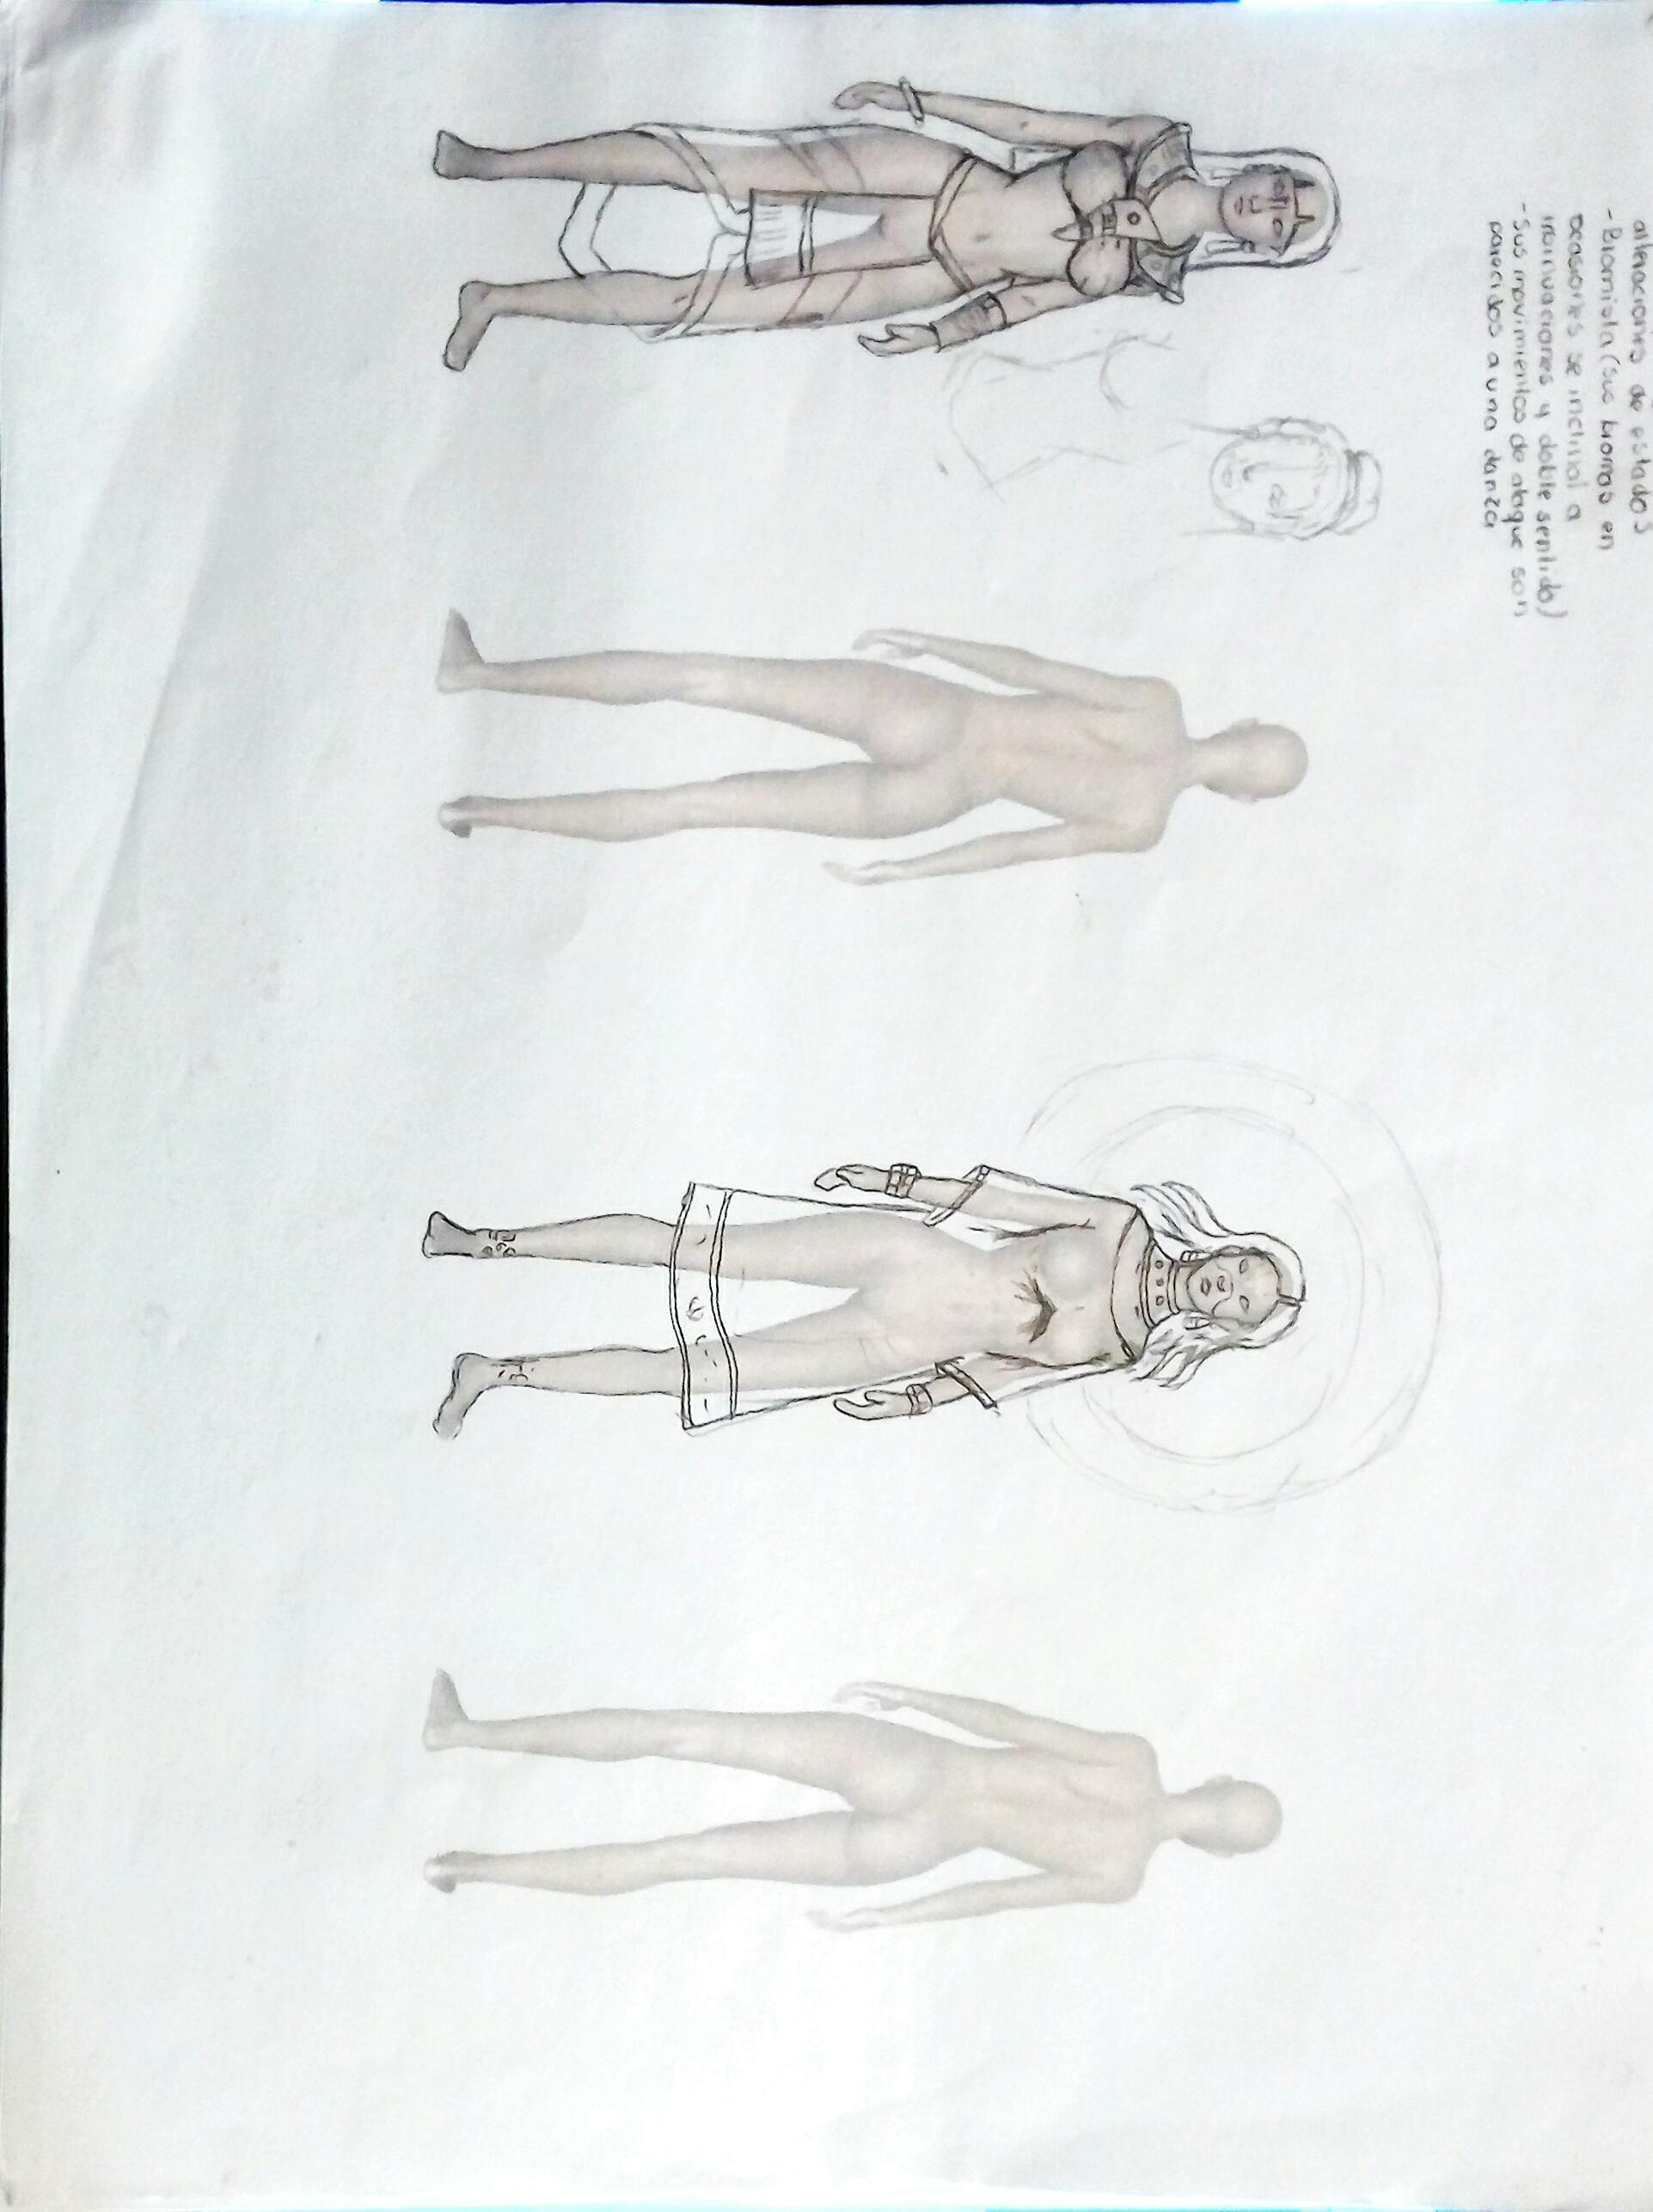
\includegraphics[height=0.2 \textheight]{Imagenes/Tlazolteotl}
	\caption{Tlazolteotl.}
	\label{fig:tlazolteotl}
\end{figure} 
\subsubsection{Concepto:}
\begin{itemize}
	\item \textbf{Historia antes del juego:}
	Luego de que uno de los antiguos guardianes del Mictlan cayera en combate durante la guerra contra los dioses del norte, Tezcatlipoca pide volutarios para tomar el puesto. Siendo Tlazoltéotl la unica en ofrecerse para tal tarea. Tlazoltéotl Elige ser guardiana del Mictlán por que tenía curiosidad sobre como eran las almas de los humanos, ya que ella considera que la verdadera cara de las personas se mostraba en la muerte.
	\\
	\par
	El papel de Tlazoltéotl en el Mictlan, ademas de proteger su nivel correspondiente, es el de purificar las almas de las personas cuyas faltas hayan sido de carácter sexual, tal como la infidelidad. A su vez, ella se encarga de darle paz a aquellas almas que hayan muerto durante agresiones de carácter sexual. 
	\item \textbf{Historia durante el juego:}
	El papel de  Tlazoltéotl en el juego se limita a ser un jefe para un nivel en especifico. Es importante remarcar que para  Tlazoltéotl, los invasores solo eran un pequeño inconveniente en un día de trabajo común.
	\item \textbf{Relaciones:}
	\begin{itemize}
		\item \textbf{Xólotl:} Considerado por Tlazoltéotl como un ser debil por el que siente un poco de pena. Encuentra un poco deprimente el hecho de que Xólotl se esfuerce demasiado por ganar la aceptación de los demás. 
		\item \textbf{Manlinalli:} Presenta un dilema para la diosa, ya que al ser su enemiga debe de derrotarla pero al observar con sus poderes los horrores a los que ha sido sometida como esclava  Tlazoltéotl desea que Malinalli encuentre pas en su corazón.
	\end{itemize}                     
\end{itemize}

\subsubsection{Encuentro:}
\begin{itemize}
	\item Su primera aparición es en la cinemática 9.
	\item Como jefe, el juagdor se enfrenta a ella en el nivel el sexto nivel del juego.
\end{itemize} 

\subsubsection{Habilidades:}
\begin{itemize}
	\item \textbf{Raíz del diablo:} Ataque que produce una confusión en el jugador, haciendo que los botones no reaccionen con las acciones que deberían.
	\item \textbf{Energía corrupta:} Esferas de energia oscura que infringen daño al jugador al hacer contacto con éste.
	\item \textbf{Circulo protector:} Utilizando energía corrupta,  Tlazoltéotl crea alrededor de ella un circulo con la capacidad de protegerla contra cualquier ataque.
\end{itemize} 
\subsubsection{Armas:}
Sin armas.
\subsubsection{Ítems:}
Sin ítems.



\subsection{Nombre: Itztlacoliuhqui}  \label{per.itztlacoliuhqui}

\subsubsection{Descripción:}
Dios de complexión corpulenta, piel blanca y de estatura alta. Tiene unas marcas negras en varias partes del cuerpo como señal de que se rebeló durante la creación del quito sol. Usa una venda en la frente para cubrir la herida causada por la flecha que le devolvió Tonatiuh. Toda a indumentaria que usa para como armadura esta hecha de oro con piedras de esmeraldas incrustadas, tal como la hombrera, el protector de cuello y pecho y los protectores de antebrazos. Porta una capa que se cruza a su cuerpo del lado izquierdo y usa un taparrabos como los que usan los nobles.
\\
\par
De carácter frio e imparcial. Itztlacoliuhqui toma su deber con seriedad y honor. Es un dios de pocas palabras, pero cuando habla acostumbra a ser directo. Prefiere las acciones a las palabras. 
\subsubsection{Status:}
Personaje no jugable.
Jefe enemigo del séptimo nivel.	  
\subsubsection{Imagen}
Ver figura \ref{fig:itztlacoliuhqui}
\begin{figure}
	\centering
	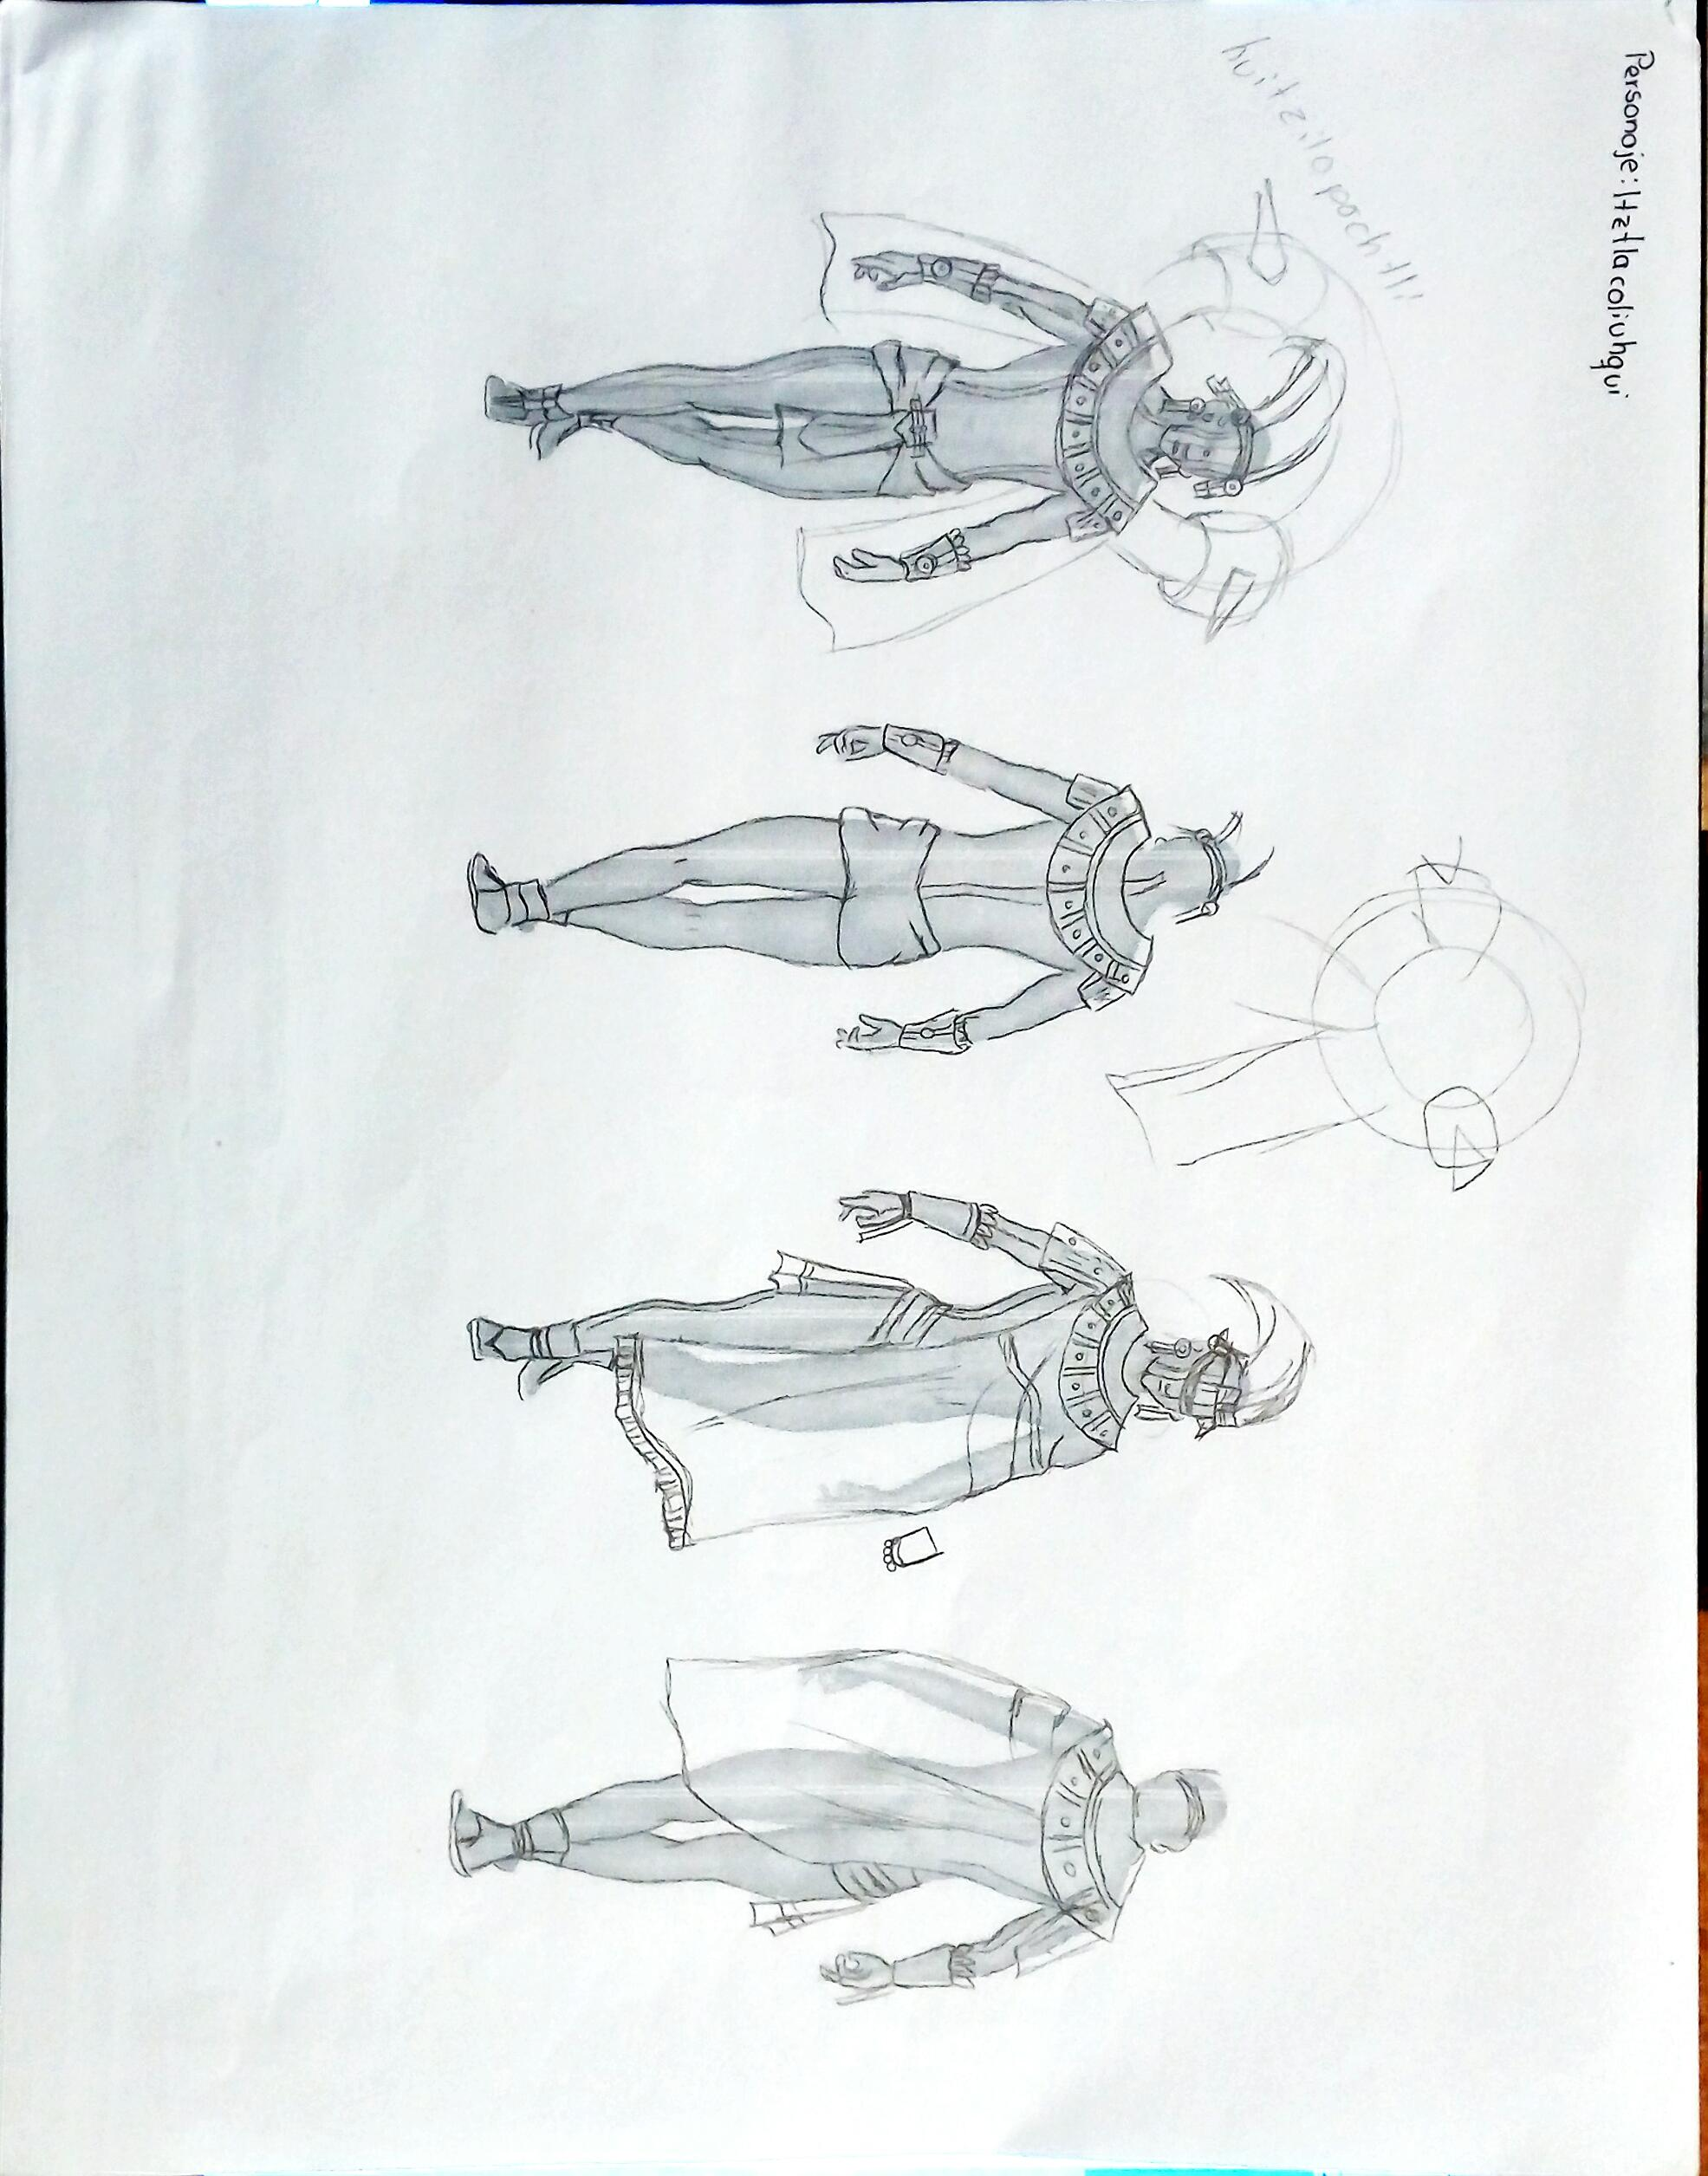
\includegraphics[height=0.2 \textheight]{Imagenes/Itztlacoliuhqui01}
	\caption{Itztlacoliuhqui.}
	\label{fig:itztlacoliuhqui01}
\end{figure} 
\subsubsection{Concepto:}
\begin{itemize}
	\item \textbf{Historia antes del juego:}
	En los tiempos anteriores al quinto Sol, el dios del castigo era conocido por el nombre de Tlahuizcalpantecuhtli y se desempeñaba como el dios de la madrugada y de Venus. De actitud alegre y amable, gozaba de una buena relación con los demás dioses; sin embargo, su amabilidad era una pantalla para ocultar la gran soberbia y orgullo que habían dentro de su corazón.
	\\
	\par
	Con la creación del quinto sol, Itztlacoliuhqui se sintió ofendido ante la nueva jerarquía divina pues consideraba que se le había relegado importancia por lo que decide derribar el quinto sol para imponer una nueva jerarquía divina.  Itztlacoliuhqui inicia su rebelión enfrentándose con Tonatiuh, pero es derrotado por éste.  Itztlacoliuhqui es castigado por sus acciones y como marca por su traición su forma y deber cambian, convirtiéndose en el Dios del castigo y siendo asignado como guardián uno de los guardianes del Mictlán.
	\\
	\par
	Como guardián del Mictlán,  Itztlacoliuhqui encuentra una manera de revindicarse en su nuevo rol. Es en el Mictlán donde conoce a Itzpapálotl. Diosa de la que se enamoraría y con quien se casaría.
	\item \textbf{Historia durante el juego:}
	Cuando Itztlacoliuhqui se entera del invasor del inframundo no muestra la más mínima señal de preocupación pues no lo considera una amenaza real, así que decide seguir con la cotidianidad de sus tareas ignorando un poco las ordenes de Mictlantecutli.
	\\
	\par
	Cuando se entera de la caída de Itzpapalotl, el deber deja de tener importancia para él y por primera vez en mucho tiempo Itztlacoliuhqui se deja gobernar por sus emociones. El deseo de recuperar la energía de Itzpapalotl para restaurarla se anteponga a su calma y sentido del honor.
	\\
	\par
	Cuando Itztlacoliuhqui se encuentra a Xolotl y Malinalli, Xolotl trata de convencerlo de que se una a él y a cambio de su ayuda restaurara la energía de Itzpapalotl. El dios del castigo se niega a escuchar a Xolotl y se transforma en un monstruo gigante para destruir a sus enemigos. Al final es derrotado por ella.
	\item \textbf{Relaciones:}
	\begin{itemize}
		\item \textbf{Itzpapalotl:} Es su esposa y la única a la que le ha demostrado calidez después de su enfrentamiento contra Tonatiuh. Itztlacoliuhqui ama a Itzapapalotl, estando ella por sobre el deber. Cuando ella es destruida por Xolotl, el deber y el honor dejan de tener sentido Itztlacoliuhqui; ya que ¿de qué le servía el honor y el deber si no había podido proteger a quien más amaba?
		\item \textbf{Xolotl: } Itztlacoliuhqui percibe a Xolotl como un dios egoísta y cobarde, pero a su vez siente pena por él ya que Itztlacoliuhqui es capaz de percibir el miedo y el vacío que habita en el corazón de Xolotl. 
	\end{itemize}			  
\end{itemize}

\subsubsection{Encuentro:}
\begin{itemize}
	\item Su primera aparición es en la cinemática 9.
	\item Como jefe, el jugador se enfrenta a él en el séptimo nivel del juego.
\end{itemize} 

\subsubsection{Habilidades:}
Como Dios del castigo, el pecado, la obsidiana y la desgracia humana, Itztlacoliuhqui puede realizar ataques que generen desastres naturales:
\begin{itemize}
	\item \textbf{LLuvia de lava:} caen bolas de lava con una gran capacidad de daño.
	\item \textbf{Manotazo:} Genera una onda expansiva que deforma el duelo provonado una oleada de rocas.
	\item \textbf{Lluvia de flechas:} Como su nombre lo dice, provoca una lluvia de flechas, este es el ataque de Itztlacoliuhqui que genera el menor nivel de daño. 
\end{itemize}
\subsubsection{Armas:}
\textbf{Arco solar:} Arma legendaria que Itztlacoliuhqui usaba desde antes del quinto Sol, siendo éste el único objeto que se le permiti conservar de su antigua identidad. Es un arco de gran alcance, permite disparar flechas con la capacidad de destruir mundos enteros. 
\subsubsection{Ítems:}
Sin ítems

\subsection{Nombre: Nexoxcho}  \label{per.nexoxcho}
\subsubsection{Descripción:}
Nexoxcho no posee una forma definida, su fisico depende de quien lo mire pues encarna los miedos más profundos de las personas.
\\
\par
En su encuentro contra Malinalli, Nexoxcho adopta la forma del Padre de ésta pero en un estado de corrupción y degradación espiritual. En esta forma el se muestra sin ojos, con las heridas de puñaladad altamente visibles y sin un corazón. De sus heridas brota un liquido negro que simula la corrupción en el alma. 
\\
\par
Nexoxcho es un dios callado y tímido. Al ser consciente de los daños que puede causarle a la psique de los Dioses, evita toparse con los demás por lo que es un dios bastante solitario. No acostumbra a luchar físicamente, el efecto que tienen sus poderes usualmente le garantiza la victoria contra cualquier enemigo.         
\subsubsection{Status:}
Personaje no jugable.
Jefe del octavo nivel del Mictlán.
\subsubsection{Imagen}
\subsubsection{Concepto:}
\begin{itemize}
	\item \textbf{Historia antes del juego:}
	Nexoxcho se ofrece de manera voluntaria a ser uno de los guardianes del Mictán durante los tiempos de restauriacion del orden luego de las rebeliones que se produjeron por la creación del quinto Sol. Pues consideraba que sus habilidades eran más útiles para los demás dioses en el Mictlan que en los trece cielos donde podía lastimar a alguien si querer.
	\item \textbf{Historia durante el juego:}
	Al ver que los demás guardianes eran derrotados sin mayor problema, Nexoxcho comprende que es su responsabilidad  absoluta frenar el avance de Xólotl.
	\item \textbf{Relaciones:}
	\begin{itemize}
		\item \textbf{Xólotl:} Nexoxcho considera a Xólotl como un ser mal agradecido e infantil. Desde su punto de vista Xólotl no tiene motivos para estar molesto. 
		\item \textbf{Nota:} Nexoxcho no puede relacionarse con los demás Dioses debido a sus poderes por lo que no goza de ningún vinculo con el resto. 
	\end{itemize}                     
\end{itemize}

\subsubsection{Encuentro:}
\begin{itemize}
	\item Su primera aparición es en la cinemática 9.
	\item Como jefe, el juagdor se enfrenta a él en el octavo nivel del juego.
\end{itemize}

\subsubsection{Habilidades:}
Nexoxcho puede ver los miedos reales de las personas y convertirlos en peligrosas ilusiones en donde atrapa a quien lo mire.  

\subsubsection{Armas:}
Sin armas.
\subsubsection{Ítems:}
Sin ítems.

\subsection{Nombre: Mictlantecutli}  \label{per.mictlantecutli}
\subsubsection{Descripción:}   
Su figura es la de un esqueleto cuya calavera esta decorada con puntura morada de guerra. Porta un penacho de oro puro que refleja su condición como gobernante del Mictlán. El resto de su vestimenta emula una armadura de guerrero. Porta unas hombreras de oro con esmeraldas incrustadas, las hombreras se incrustan en un protector para el pecho que tiene diferentes grabados, mientras que sus protectores para los brazos están hechos de esmeraldas. Usa un taparrabo idéntico al que usan los tlatoanis, éste es sujetado por un delgado cinturón de oro. Mictlantechtli usa, ademas, una capa y zapatos característicos de quien es parte de la nobleza.
\\
\par
De carácter temperamental, le gusta tener el control de la situación por lo que es inusual verlo fuera de su zona de confort. Su ordenes son absolutas y no aceptara segundas opiniones, llegando incluso a destruir a aquellos que busquen alterar el orden. Desprecia las emociones humanas y considera que los humanos son criaturas pasionales y primitivas que no son conscientes del tiempo que tiene hasta que ya es tarde. Es un ser muy apegado a sus pertenencias. 
\subsubsection{Status:}
Personaje no jugable.
Jefe del décimo nivel, es el jefe final del juego.
\subsubsection{Imagen}
Ver figura \ref{fig:mictlantecutli}
\begin{figure}
	\centering
	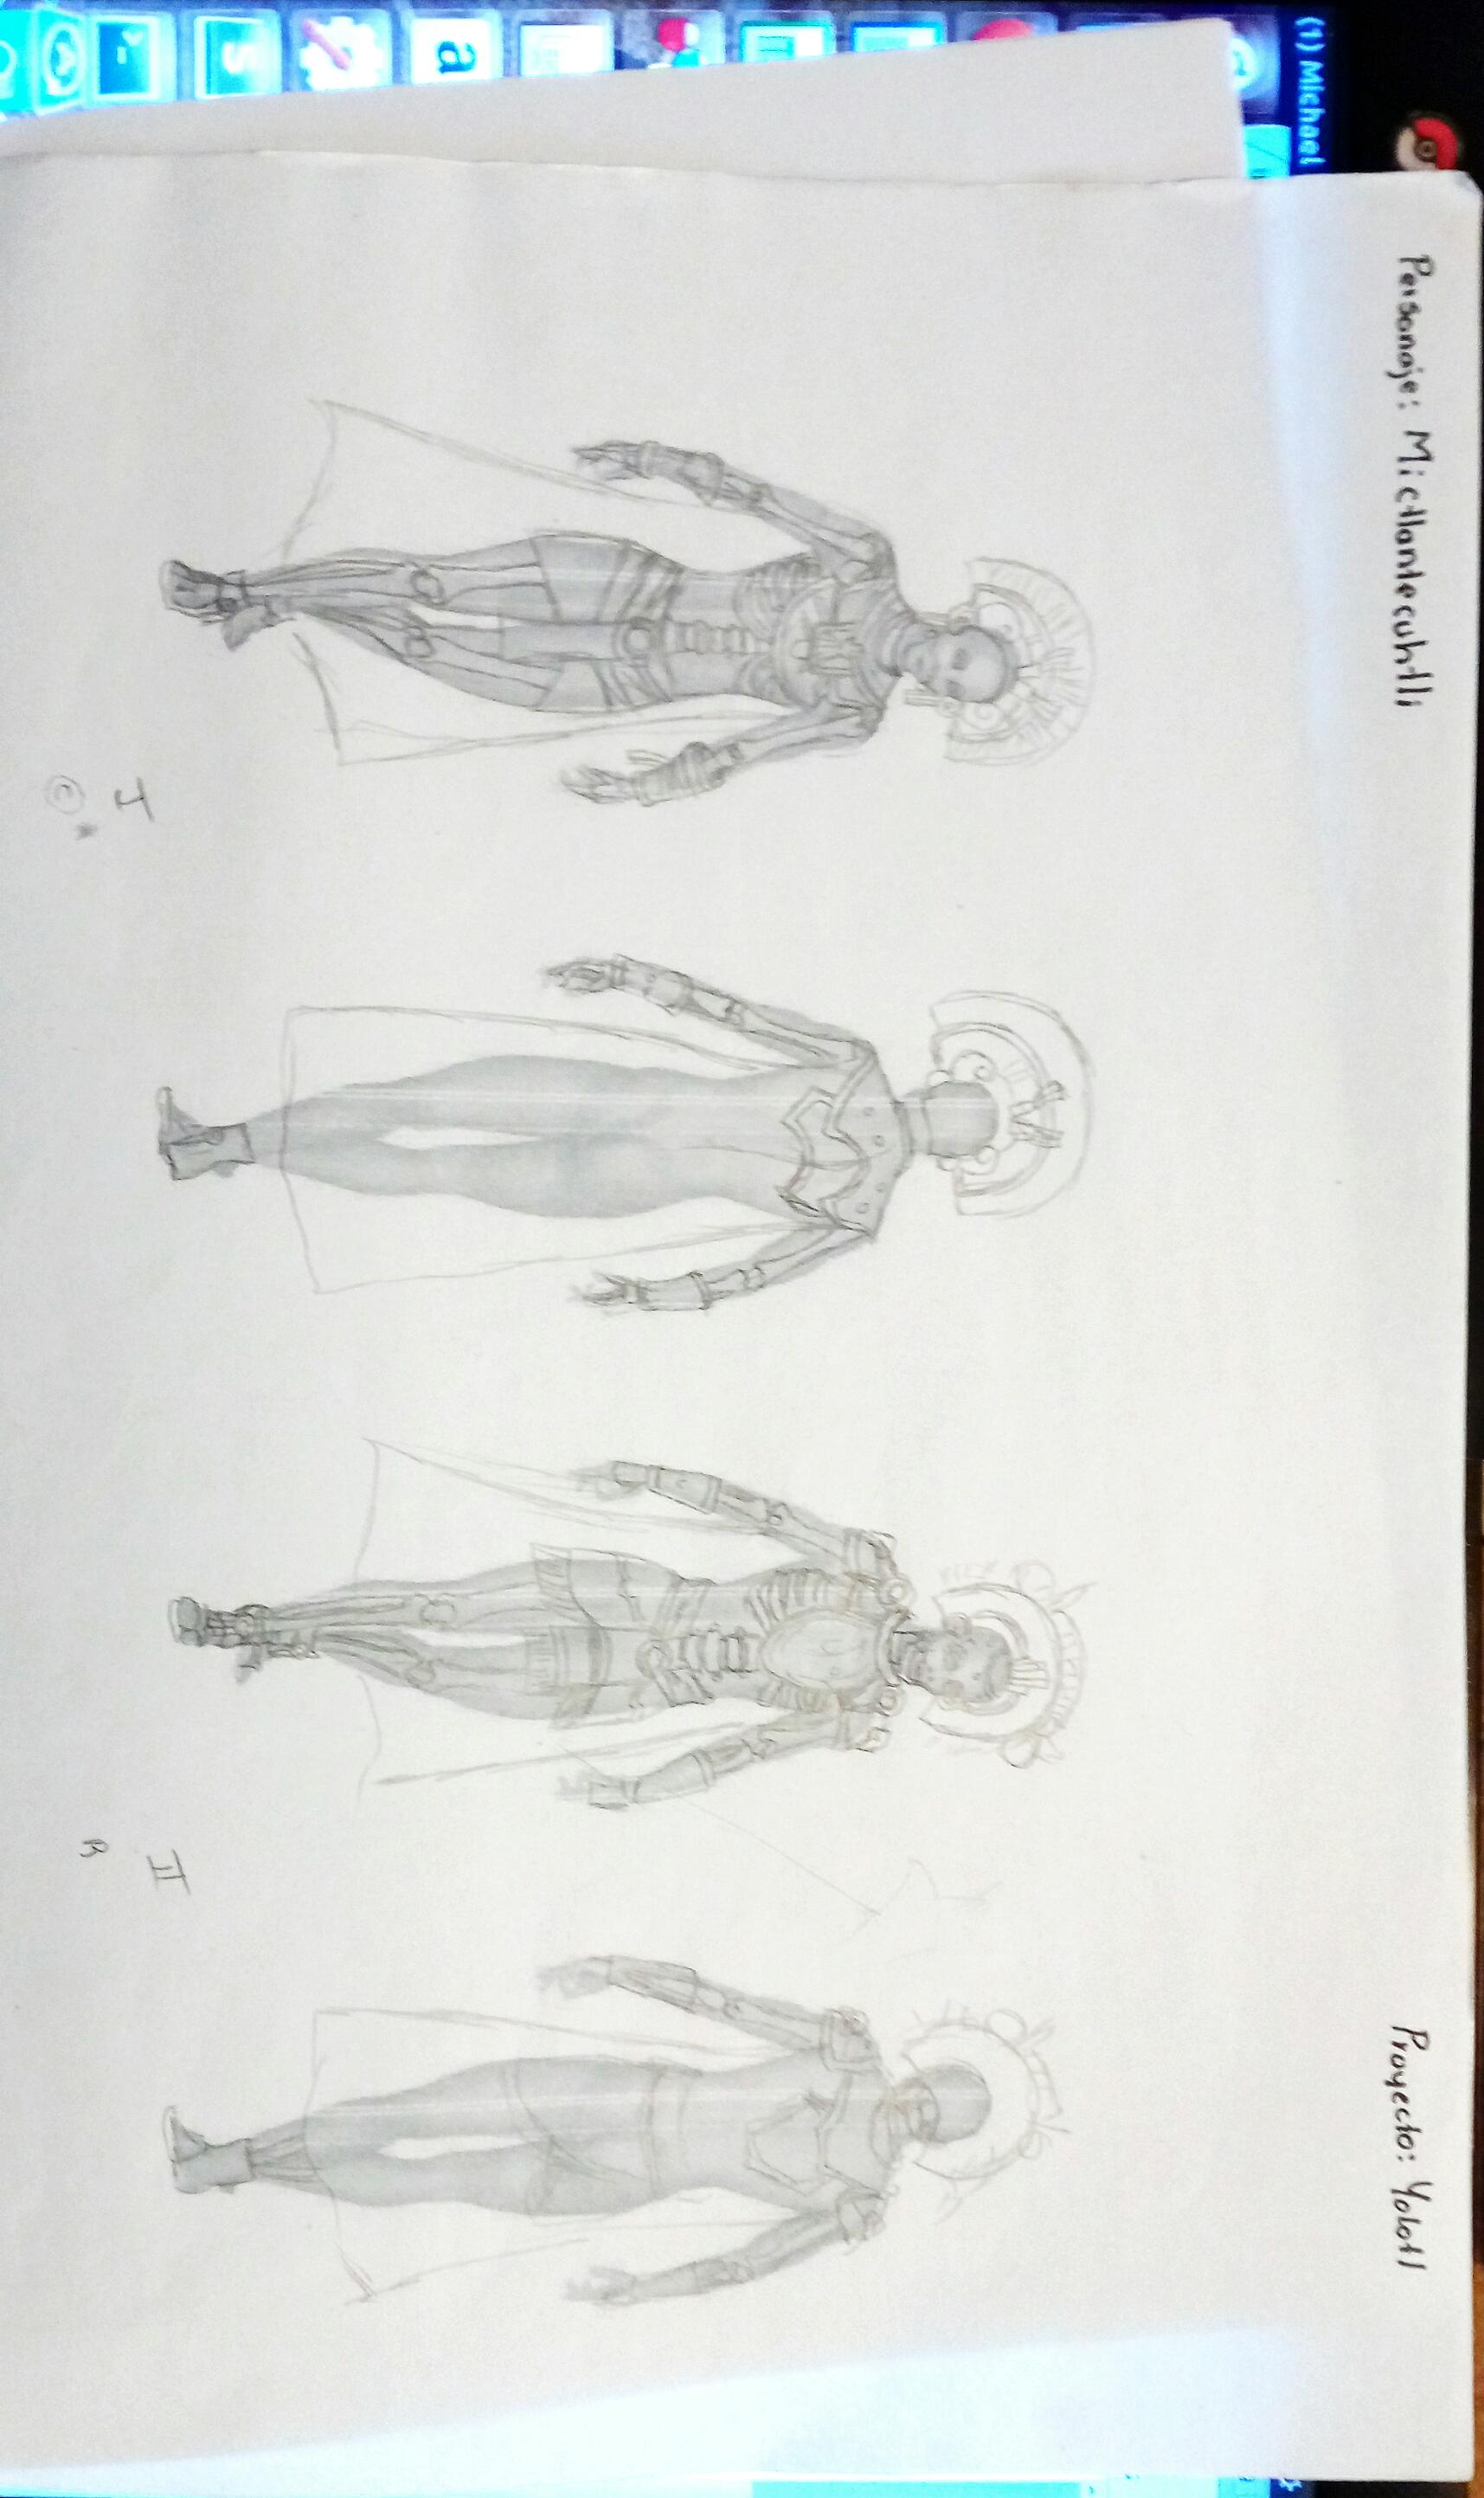
\includegraphics[height=0.2 \textheight]{Imagenes/Mictlantechtli}
	\caption{Mictlantecutli.}
	\label{fig:mictlantecutli}
\end{figure} 
\subsubsection{Concepto:}
\begin{itemize}
	\item \textbf{Historia antes del juego:}
	Después de la creación del quinto Sol,  Mictlantechtli se negó a dar los huesos de los antiguos hombres para rehacer la humanidad, pues consideraba que la humanidad como un capricho de Quetzalcóatl. Si bien al final termina ayudando, nunca perdonara que Quetzalcóatl y Xólotl robaron los huesos de los antiguos hombres del inframundo.
	\\
	\par
	El nuevo orden que instauran los dioses con el quinto sol, trae nuevas responsabilidades para  Mictlantechtli. Su rol no solo sería garantizar la purificación de las almas de los muertos, ahora también debería encargarse de la seguridad de los trece cielos al evitar que cualquiera pudiera entrar al Mictlán. Por consejo de  Mictecacíhuatl,  Mictlantechtli le exige a los dioses gobernantes de los trece cielos la presencia de nuevos guardianes para los niveles del Inframundo; desafortunadamente no todos los aspirantes logran pasar los requisitos de Mictecacíhuatl y  Mictlantechtli, por lo que Mictlantechtli toma los huesos de diferentes animale smuertos y crea a Xochitónal. Completando así los nueve guardianes.
	\\
	\par
	Luego del exilio de Quetzalcóatl, Mictlantechtli le deja en claro a Tezcatlipoca que a él le da igual quien gobierne los trece cielos siempre que él sea quien gobierne el Mictlán, advirtiendole que él no va a tolerar que se desate una guerra civil entre los dioses por los conflictos entre Tezcatlipoca y Quetzalcóatl. 
	\item \textbf{Historia durante el juego:}
	La muerte de Xochitónal toma por sorpresa a Mictlantechtli, pero debe de dejar a un lado el poco afecto que tenía por su creación para dar nuevas ordenes para mantener el orden de sus dominios. A medida de que cada uno de los guardianes va cayendo en el campo de batalla,  Mictlantechtli comienza a aceptar la derrota, sin embargo su orgullo le impide aceptarlo abiertamente. 
	\item \textbf{Relaciones:}
	\begin{itemize}
		\item \textbf{Mictecacíhuatl:} Esposa de Mictlantechtli. El lazo matrimonial que los une no es producto del amor, sino del deber. Ambos dioses colaboran juntos para mantener en orden el Mictlán. Si bien Mictlantechtli no ama a su esposa, si tiene un gran afecto y respeto. Este afecto lo lleva a pedirle a  Mictecacíhuatl que se retire del inframundo y vaya a los trece cielos para mantenerla a salvo.
		\item \textbf{Quetzalcóatl:}  Mictlantechtli tiene un conflicto no resuelto con este dios, luego de que Quetzalcóatl robara los huesos de los antiguos hombres.
		\item \textbf{Xólotl:}  Desde el punto de vista de Mictlantechtli, Xólotl es un cobarde, resentido que busca alterar el orden por mera perversión.
		\item \textbf{Malinalli:}  Mictlantechtli ve en Malinalli una niña pequeña, asustada, obsesionada con las personas que ha perdido e incapaz de ver por si misma que Xólotl solo la utiliza. 
	\end{itemize}                     
\end{itemize}

\subsubsection{Encuentro:}
\begin{itemize}
	\item Su primera aparición es en la cinemática 9.
	\item Como jefe, el jugador se enfrenta a él en el décimo nivel del juego.
\end{itemize} 

\subsubsection{Habilidades:}
\begin{itemize}
	\item \textbf{Todos los hombres del rey:} Con este ataque,  Mictlantechtli invoca a varios de los enemigos normales que habitan el Mictlán para que se enfrenten al jugador mientras  Mictlantechhtli desaparece.
	\item \textbf{Fuego mortífero:}  Mictlantechtli  lanza poderosas esferas de fuego verde.
	\item \textbf{Penitencia:}  Mictlantechtli se eleva en el aire haciendo que salgan huesos filosos del suelo.
\end{itemize}  
\subsubsection{Armas:}
Sin armas.
\subsubsection{Ítems:}
Sin ítems
        \subsubsection{Habilidades:}
\begin{itemize}
	\item Mictecacíhuatl no es un jefe o enemigo a enfrentar por lo que no tiene una lista de habilidades a programar.
\end{itemize}  
        \subsubsection{Armas:}
Sin armas.
        \subsubsection{Ítems:}
Sin ítems
        \subsubsection{Personaje No-Jugable}
Nunca se encuentra con Malinalli en todo el juego, pero ha oido hablar de ella por Tepeyóllotl, el papel de Mictecacíhuatl es el de coordinar las acciones de los guardianes del inframundo y servir como un puente en la comunicación que existe entre Mictlantechtli y ellos.


\subsection{Nombre: Mictecacíhuatl}  \label{per.mictecacihuatl}
\subsubsection{Descripción:}   
Al igual que Mictlantechtli,  Mictecacíhuatl es un esqueleto. Su vestimenta es parecida a la que usaban las damas de alta cuna en las cortes mexicas, con la diferencia de que su huipil no le cubre todas las piernas y es ligeramente más ajustado a la altura del pecho. Usa un collar de oro que cubre la mitad de su pecho. Arriba del huipil viste una capa que tiene una caída en V. Completando su conjunto de joyería lleva un brazalete con esmeralda incrustadas en la mano derecha y dos pulseras de oro en la izquierda. Porta un penacho de oro más discreto que el de su esposo. Usa un par de sandalias hechas de tela.
\\
\par
Al ser una de las diosas de mayor jerarquía,  Mictecacíhuatl es una mujer de  carácter fuerte y marcado liderazgo, llegando a tomar las riendas del Mictlán cuando las decisiones de  Mictlantechtli no son las mejores a seguir. Es una mujer fina y educada, de andar delicado. Jamas alzará la voz para que los demás escuchen sus palabras, pero posee la suficiente soltura y la suficiente habilidad de oratoria para que los demás siempre darse a escuchar. Mictecacíhuatl posee un fuerte sentido de la estrategia, siendo una de sus cualidades de mayor peso el hecho de que sabe elegir al Dios que que cumplirá mejor con el mejor desempeño para cada puesto. 
\subsubsection{Status}
Personaje no jugable.
Nunca se encuentra con Malinalli en todo el juego, pero ha oido hablar de ella por Tepeyóllotl, el papel de Mictecacíhuatl es el de coordinar las acciones de los guardianes del inframundo y servir como un puente en la comunicación que existe entre Mictlantechtli y ellos.
\subsubsection{Imagen}
Ver figura \ref{fig:mictecacihuatl}
\begin{figure}
	\centering
	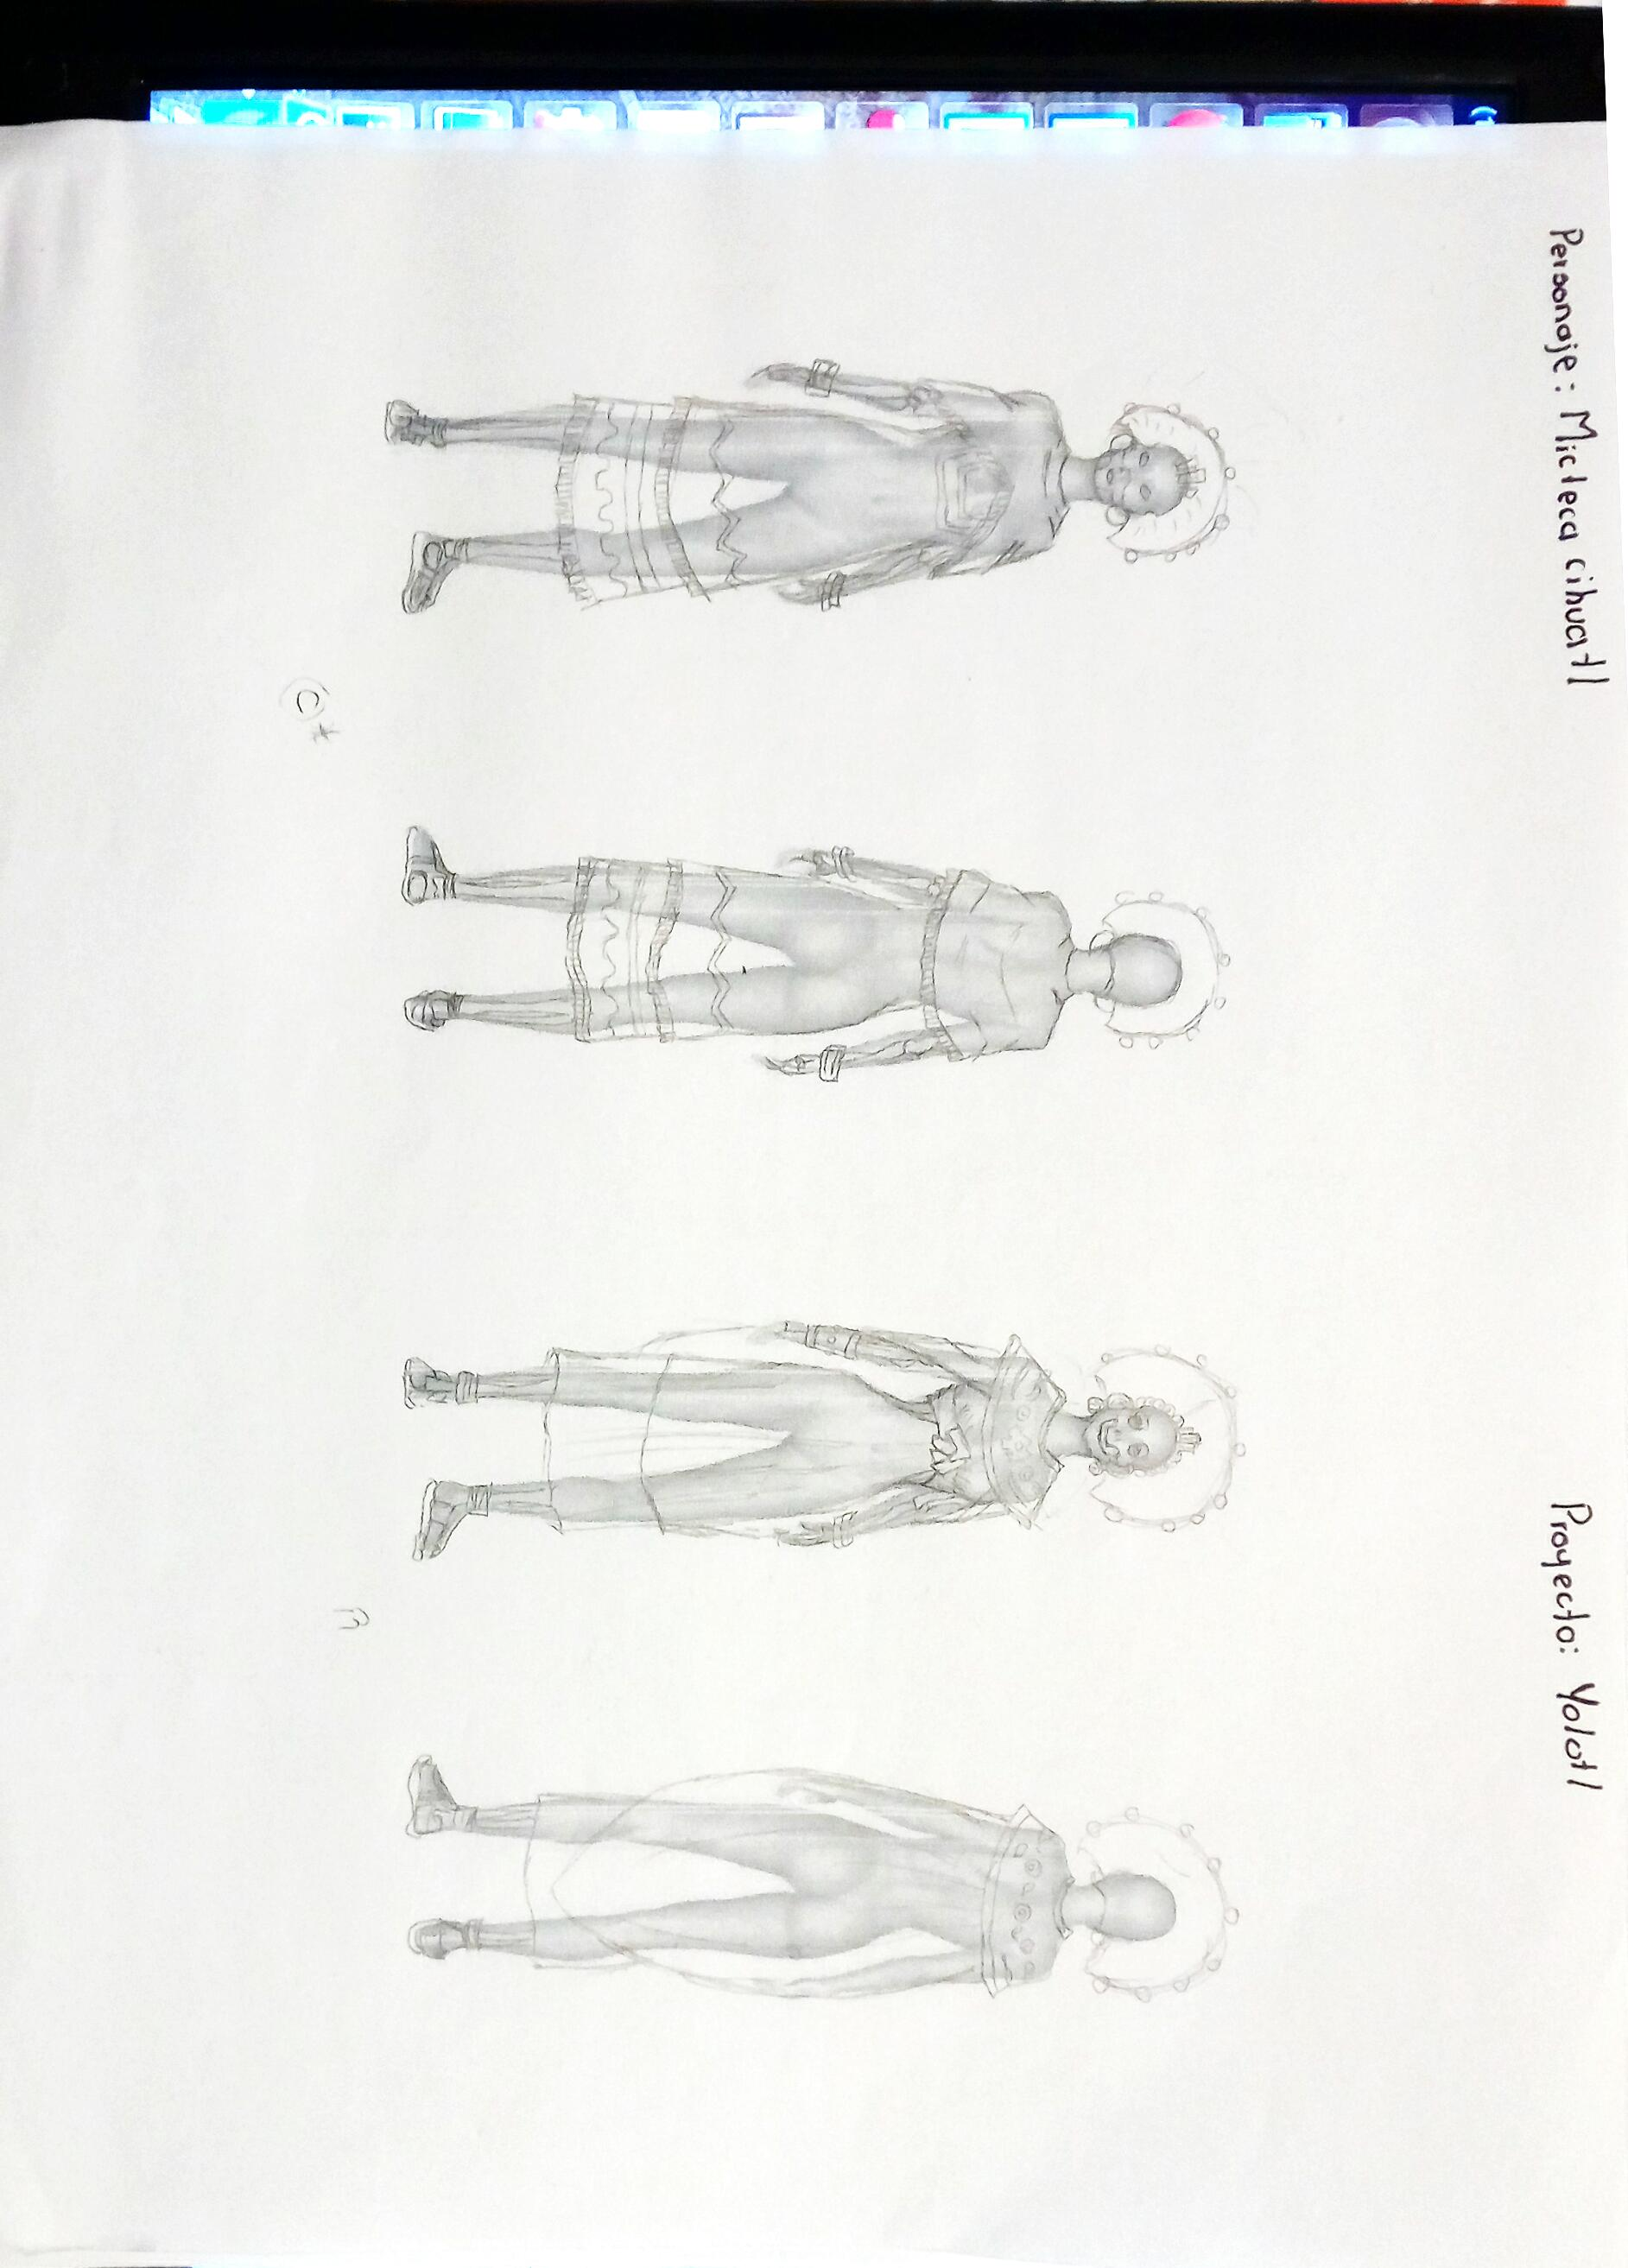
\includegraphics[height=0.2 \textheight]{Imagenes/Mictecacihuatl}
	\caption{Mictecacihuatl.}
	\label{fig:mictecacihuatl}
\end{figure} 
\subsubsection{Concepto:}
\begin{itemize}
	\item \textbf{Historia antes del juego:}
	Nacida como la contraparte femenina de  Mictlantechtli, Mictecacíhuatl comprendio desde el inicio de su existencia cual era su rol como Diosa. Considerándose a sí misma como una reina que debía gobernar.  Mictecacíhuatl ejerce su gobierno sobre el Mictlán al tener la ultima palabra sobre los asuntos de mayor importancia, fungiendo como un puente que comunica el noveno nivel del Mictlán con el resto de los niveles y con los trece cielos.
	\\
	\par
	En diferentes ocasiones Mictecacíhuatl ha conspirado contra su esposo, llegando a enfrentarse a él para mantener el orden en el Mictlán; sus enfrentamientos siempre han surgido por la falta de liderazgo objetivo por parte de Mictlantechtli, ya que mientras  Mictlantechtli tiende a llevarse más por su orgullo y su temperamento a la hora de tomar decisiones, Mictecacíhuatl se guia más por un análisis de la situación.
	\item \textbf{Historia durante el juego:}
	Mictecacíhuatl ve con curiosidad el ataque de Xólotl, siendo la primera en darse cuenta que el ataque al Mictlán tenía connotaciones más fuertes de lo que parecían a primera instancia. A pesar de contar con todos los recursos para frenar a Xólotl, Mictecacíhuatl decide dejarlo avanzar, limitandose a cumplir con las ordenes de Mictlantechtli aun sabiendo que la estrategia de éste no era la más acertada. Ella deja que el Mictlán caiga pues confiaba plenamente en que en los trece cielos seran capaces de frenar a Xólotl, por lo que una vez vencido Xólotl y sin  Mictlantechtli, ella podría gobernar el Mictlán.
	item \textbf{Relaciones:}
	\begin{itemize}
		\item \textbf{Mictlantechtli:} Esposo de Mictecacíhuatl. Diversas malas decisiones que  Mictlantechtli ha tomado a lo largo de su gobierno en el Mictlán han llevado a Mictecacíhuatl a dejar de verlo como un líder.  
		\item \textbf{Xólotl:} Persivido como un traidor,la presencia de Xólotl le permitirá a Mictecacíhuatl iniciar su propia misión para hacerse del control del Mictlán. 
	\end{itemize}                     
\end{itemize}

\subsubsection{Encuentro:}
\begin{itemize}
	\item Su primera aparición es en la cinemática 9.
\end{itemize} 

\subsubsection{Habilidades:}
\begin{itemize}
	\item Mictecacíhuatl no es un jefe o enemigo a enfrentar por lo que no tiene una lista de habilidades a programar.
\end{itemize}  
\subsubsection{Armas:}
Sin armas.
\subsubsection{Ítems:}
Sin ítems


\subsection{Nombre: Tenépal}  \label{per.tenepal}
\subsubsection{Descripción:}   
Hombre de mediana edad de piel morena, ojos café oscuro y cabello largo peinado en una media cola. No usa penacho para denotar su posición como gobernante, debido a que considera el accesorio como estorboso y pesado por lo que solo un par de plumas de Quetzal son utilizadas como símbolo de su poder. Viste una capa algodón fino y un taparrabo de manta con grabados de colores. Usa unas sandalias características de un guerrero mexica. Porta un par de brazaletes en cada brazo una en las muñecas y otra en el biceps.
\\
\par
De carácter fuerte y decidido, se muestra constantemente preocupado por su hija y por su pueblo. A pesar de ser un cacique al servicio del imperio mexica, difiere en cuanto a los métodos que tiene el imperio para gobernar a sus territorios conquistados. Considera el deber y el honor como sus principales valores pero también comprende que no siempre se puede seguir el honor al pie del a letra ya que la moral del mundo no funciona en blanco sino a escala de gises. 
\subsubsection{Status:}
Personaje no jugable.
Aparece solo en cinemáticas, es la motivación de Malinalli para continuar cuando la situación se poner dura. 
\subsubsection{Imagen}
Ver figura \ref{fig:tenepal}
\begin{figure}
	\centering
	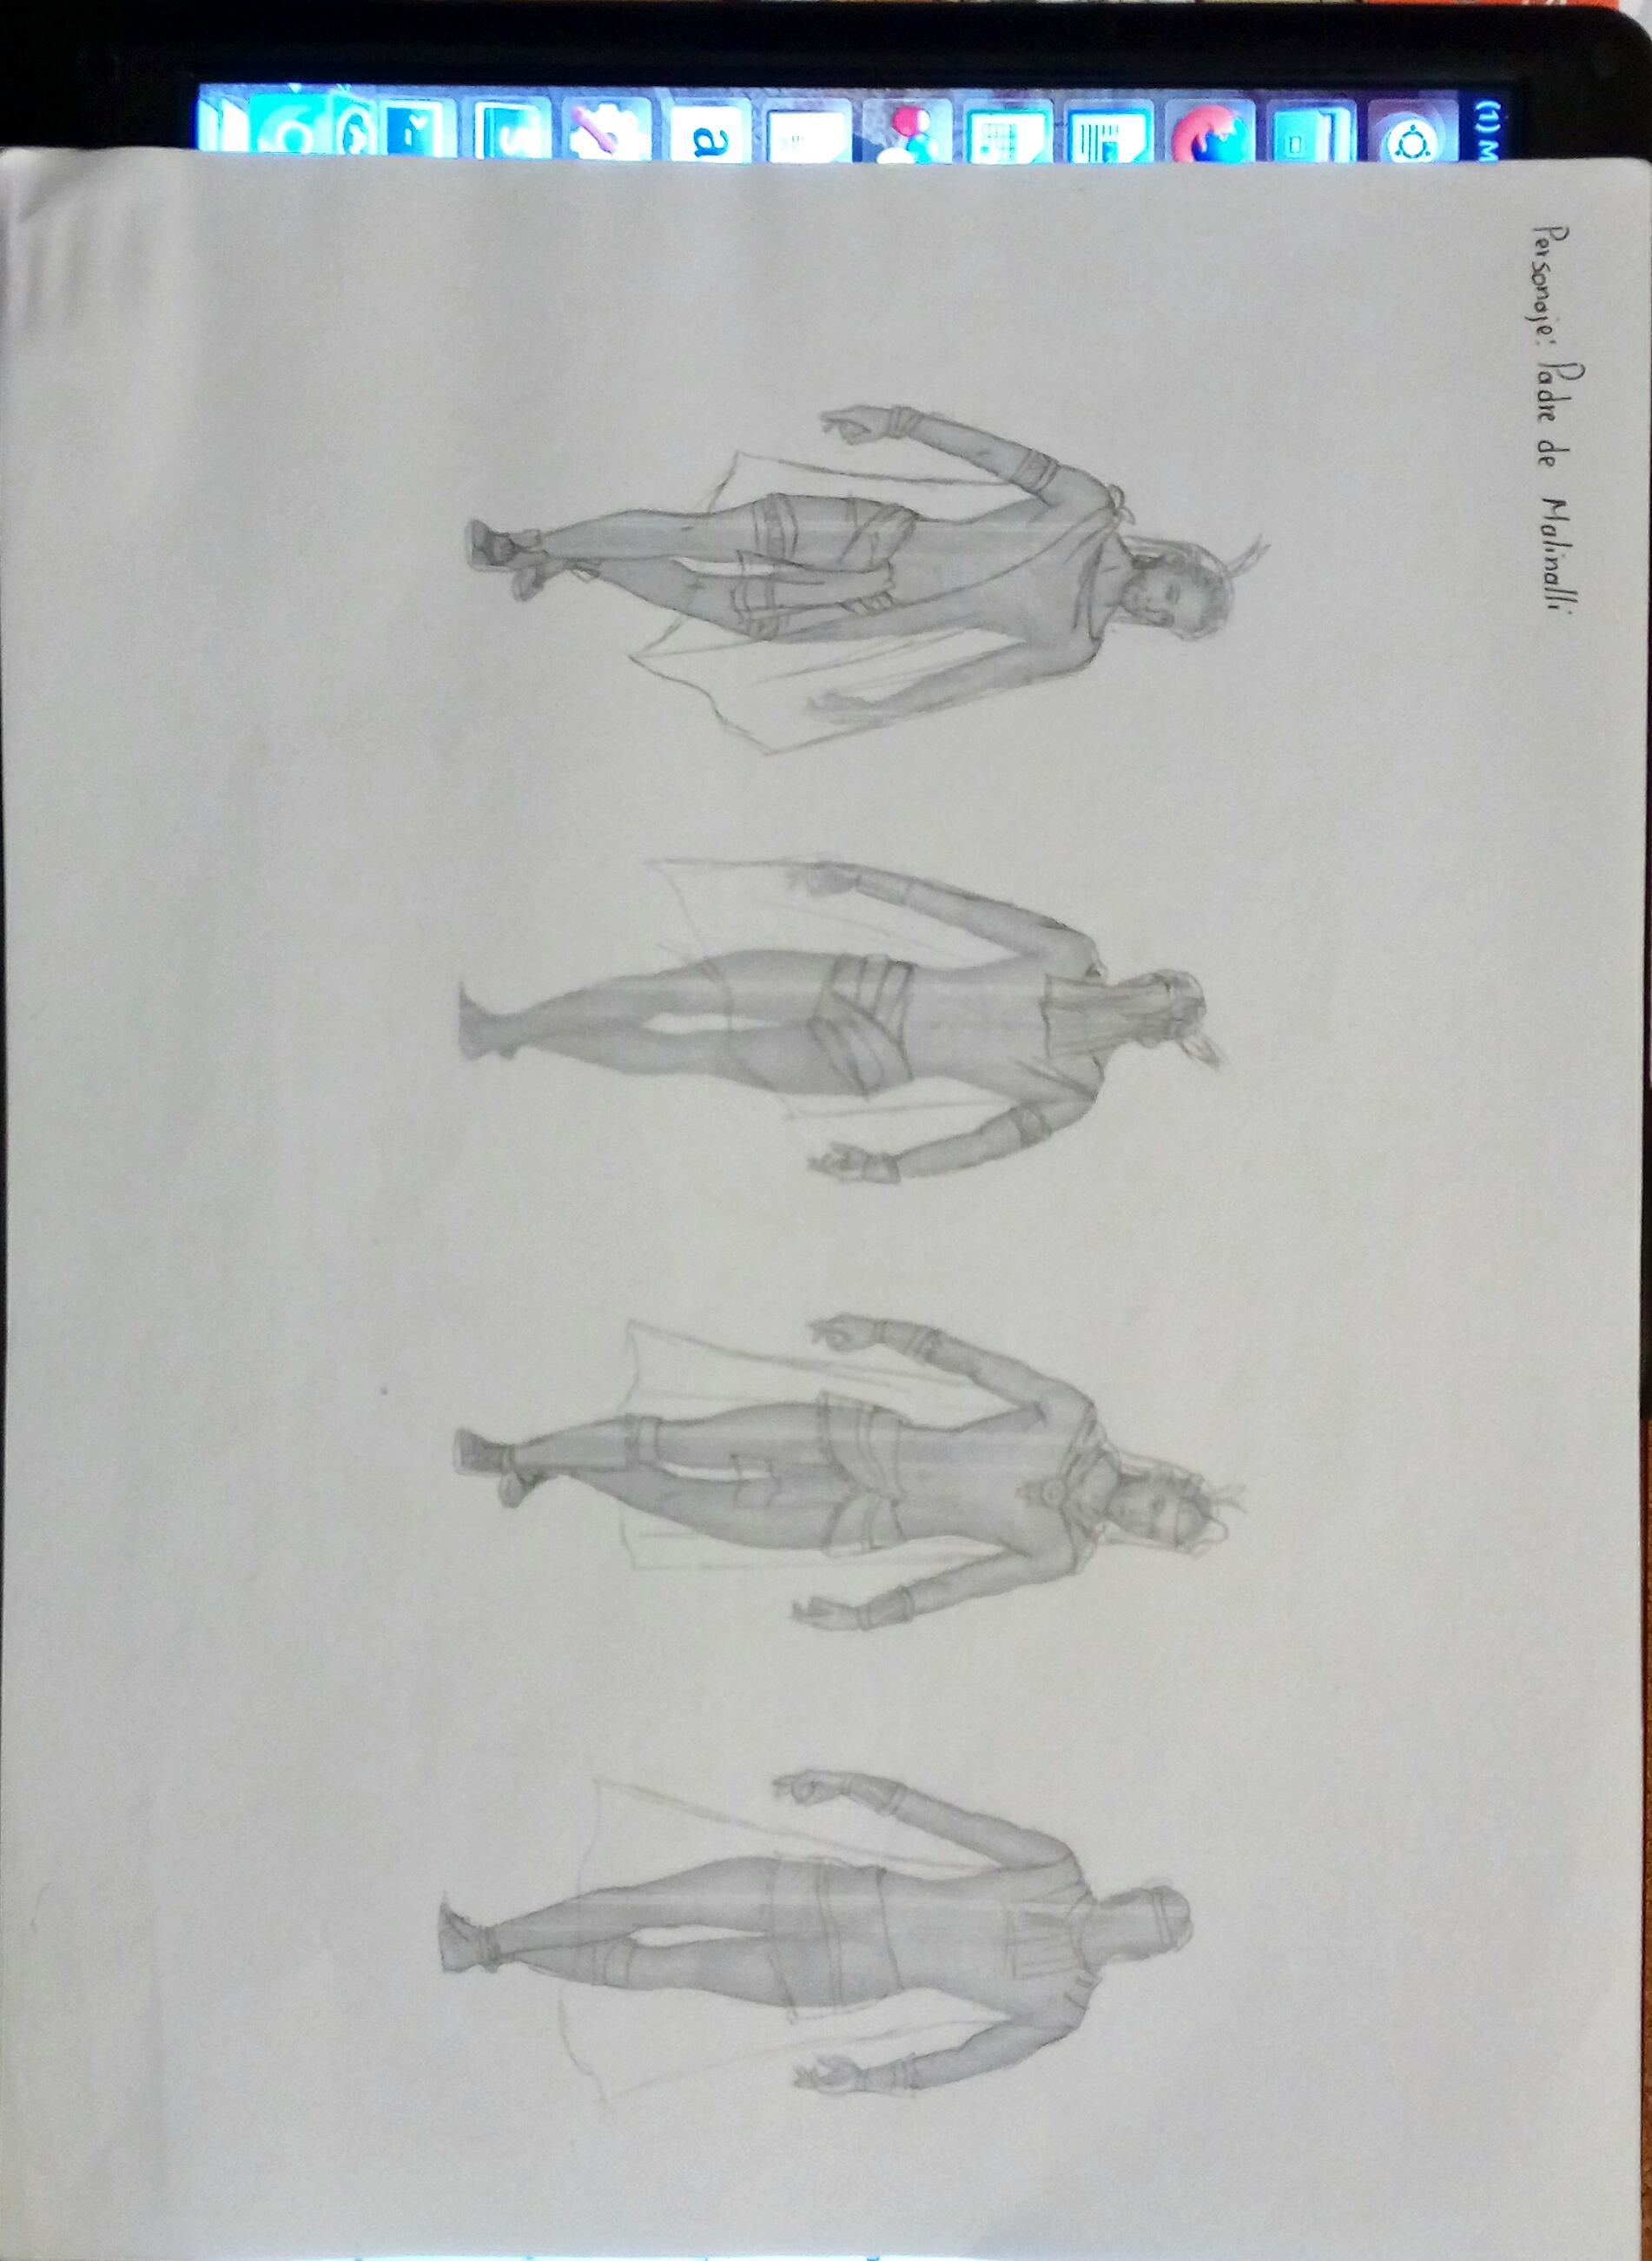
\includegraphics[height=0.2 \textheight]{Imagenes/Tenepal}
	\caption{Tenepal.}
	\label{fig:tenepal}
\end{figure} 
\subsubsection{Concepto:}
\begin{itemize}
	\item \textbf{Historia antes del juego:}
	Tenépal nació dentro de una familia noble y bien posicionada pero fue gracias a sus dotes como guerrero y a su gran carisma como líder que consiguió escalar socialmente hasta convertirse en el cacique de Oluta. Por consejo de su corte decide tomar por esposa a Cimatl, hermosa mujer de noble linaje que le permitió formar formar alianzas comerciales con diferentes pueblos de la región. Varios años despues de contraer nupcias, la pareja tuvo a su primera y única hija: Malinalli. 
	\\
	\par
	Durante los años venideros al nacimiento de su hija, Tenépal viajaría por distinto territorios del imperio, esto lo llevaría a concluir que la situación del imperio era demasiado frágil al no contar con una verdadera unión entre sus territorios, haciéndolo propicio de ser invadido por cualquier potencia con la suficiente astucia como para unir a los pueblos subyugados. En uno de sus viajes, Tenépal conoce a una sacerdotisa que clamaba ver el futuro, quien tras conocerlo le cuenta la profecía del legendario territorio conocido como el ombligo de la luna y como este sería el territorio que unificaría todos las culturas. Tras contarle la leyenda del ombligo de la luna, la sacerdotisa le asegura a Tenépal que su descendencia jugara un papel vital en la formación de este territorio. Es tras esta revelación que Tenépal decide iniciar su campaña para unificar los territorios del sur del imperio para iniciar una rebelión.
	\\
	\par
	La rebelión de Tenépal inicia como una conspiración secreta entre los gobernantes, los guerreros y la nobleza de los territorios sureños; sin embargo, todos los conspiradores son traicionados y mandados a ejecutar en secreto por el Tlatoani.  
	\item \textbf{Historia durante el juego:}
	Cuando el juego inicia Tenépal ya esta muerto, pero su recuerdo acompañara a Malianlli por toda su travesía, siendo su constante aliento y animo en los momentos difíciles.
	\item \textbf{Relaciones:}
	\begin{itemize}
		\item \textbf{Cimatl:} Esposa de Tenépal, ambos se casan por conveniencia sin poder formar un lazo emocional en los años que duraría su matrimonio. Su único punto en común es Malinalli, quien es a momentos utilizada por Cimatl para obtener lo que desea de su esposo.
		\item \textbf{Malinalli:} Hija de Tenépal, es la persona más importante en su vida y la persona a la que más ama. Tenépal cree totalmente en Malinalli. 
	\end{itemize}                     
\end{itemize}

\subsubsection{Encuentro:}
Aparece por primera vez en la cinemática 7.
\subsubsection{Habilidades:}
Tiene las habilidades combativas de un un guerrero humano. Su principal habilidad es su capacidad de planear y de convencimiento.
\subsubsection{Armas:}
En sus años como guerrero usaba una Macuahuitl para enfrentarse a sus enemigos.
\subsubsection{Ítems:}
Sin ítems


\subsection{Nombre: Cimatl}  \label{per.cimatl}
\subsubsection{Descripción:} 
Mujer de edad media. Cimatl es una mujer bella, de piel morena y cabello largo. Lleva el pelo recogido en una especie de chongo como el que usaban las mujeres nobles de la capital del imperio. Viste una especie de chal que le llega hasta la altura de los codos y un huipil cuyo largo es hasta los tobillos. Una un par de pulseras de jade, una en cada mano y un collar de oro labrado por Mixtecos por lo que tiene una gran cantidad de detalles en su labrado. Ademas de eso, utiliza un par de aretes labrados en la misma zona. Porta unas sandalias que cubren la mayor parte de sus pies.
\\
\par
Cimatl es una mujer ambiciosa que se siente atraída al poder. Su deseo por el poder es tal que no durara en hacer lo que sea necesario para mantenerse en el poder y gozar de la riqueza.        
\subsubsection{Status:}
Personaje no jugable.
Es uno de los fantasmas del pasado de Malinalli.
\subsubsection{Imagen}
\subsubsection{Concepto:}
\begin{itemize}
	\item \textbf{Historia antes del juego:}
	Hija de un importante comerciante. Durante su juventud Cimatl tuvo un sin numero de pretendientes que deseaban esposarla por su gran belleza; sin embargo, Cimatl no encontraba en ninguno de sus pretendientes alguno que le garantizara una posición social de mayor rango de la que ya gozaba. Gracias a la amistad de su padre con uno de los consejeros del nuevo cacique, los padres de Cimatl arreglaron el matrimonio de su hija con el cacique. La vida matrimonial solo logro decespcionar a Cimatl, ya que ella esperaba que su esposo fuera un hombre ambicioso y en su lugar encontro un hombre preocupado por su pueblo y no en el poder. Por lo que Cimatl empieza a temer por la seguridad de su patrimonio al temer que su esposo perdiera el poder por su antitud amable.
	\\
	\par
	Después de varios años de matrimonio, Cimatl queda embarazada; a lo que ella empezaría a depositar sus esperanzas de conseguir más poder al dar a luz a un varón. Pero sus planes se ven truncados con el nacimiento de una niña. A los años que siguieron de su matrimonio, Cimatl comenzó a proponerle a su esposo la idea de conseguirle a futuro un arreglo matrimonial a Malinanlli con algún importante señor de la capital del imperio a lo que Tenépal se niega, ganandose la furia de su esposa.
	\\
	\par
	Su oportunidad para hacerse de más poder llega cuando descubre la conspiración que su esposo estaba orquestando contra el imperio. Cimatl, temerosa de que su esposo fuera descubierto y ello significara la ruina de ella, decide entregarlo al tlatoani con la condición de que ella sería la esposa del siguiente cacique.
	\\
	\par
	A los pocos meses de la muerte de su espos, Cimatl contrae nupcias con el nuevo cacique de Oluta. De este matrimonio nacería un hijo varón, que se convertiría en la llave de más poder para Cimatl. Es entonces cuando Malinalli comienza a ser una amenaza para sus pretensiones políticas por lo que decide venderla como una esclava.  
	\item \textbf{Historia durante el juego:}
	Se conocerá a Cimatl a través de los recuerdos de Malinalli ya que no tiene participación en la historia que transcurre dentro del Mictlán.
	\item \textbf{Relaciones:}
	\begin{itemize}
		\item \textbf{Tenépal:} Considerado como un hombre débil y de poca visión por su esposa. Ella lo aborrecía al ser un obstáculo a sus pretensiones de poder. 
		\item \textbf{Malinalli:} vista como el mayor fracaso de Cimatl, ya que por su condición de mujer no resultaba provechosa para mantener la posición política de su madre ni su riqueza. Con el nacimiento de su hermano, Malinalli pasa a ser una amenaza para Cimatl por lo que debe de ser erradicada.
		\item \textbf{Huenupan:} Segundo esposo de Cimatl. No guarda amor por el pero lo considera util.
	\end{itemize}                     
\end{itemize}

\subsubsection{Encuentro:}
Aparece por primera vez en la cinemática 25.
\subsubsection{Habilidades:}
Su principal habilidad es la de planear y conspirar para obtener lo que desea.
\subsubsection{Armas:}
No posee armas ni esta amaestrada en la batalla.
\subsubsection{Ítems:}
Sin ítems.


\subsection{Nombre: Huenupan}  \label{per.huenupan}
\subsubsection{Descripción:} 
Hombre de mediana edad y corpulencia delgada. De tez morena oscura y cabello largo. Usa un penacho para denotar su posición como cacique. Viste una capa de algodón fino que cuelga de sus espalada de manera recta y con un taparrabos de manta de colores. Porta dos brazaletes de diferentes acabados, uno en cada brazo. Y usa unas sandalias sencillas del color de su capa.     
\\
\par
De actitud pasiva y obediente; Huenupan carece de las actitudes para ser un lider por lo que se limita a obdecer las ordenes del imperio. 
\subsubsection{Status:}
Personaje no juegable.
Es uno de los fantasmas del pasado que atormentan a Malinalli.
\subsubsection{Imagen}
\subsubsection{Concepto:}
\begin{itemize}
	\item \textbf{Historia antes del juego:}
	Originario de una familia noble del  norte de Veracruz, logra ascender hasta cacique debido a su ciega lealtad al imperio. Acepta el puesto sin conocer las necesidades de la población, siendo su prioridad garantizar el control del imperio pero no el bienestar de su pueblo.  
	\item \textbf{Historia durante el juego:}
	Su presencia se conoce por los recuerdo de Malinalli, o tiene participación directa en la historia que sucede en el Mictlán.
	\item \textbf{Relaciones:}
	\begin{itemize}
		\item \textbf{Cimatl:} Esposa de Huenupan. Acepta casarse con ella para tomar el puesto de cacique. Debido a su personalidad pasiva, usualmente termina siendo manipulado por su esposa para que haga lo que ella desea. 
		\item \textbf{Malinalli:} No guarda ningún cariño por ella. 
	\end{itemize}                     
\end{itemize}

\subsubsection{Encuentro:}
Su primera aparición es el la cinemática 25.
\subsubsection{Habilidades:}
Es un guerrero de pocas habilidades. 
\subsubsection{Armas:}
Sin armas.
\subsubsection{Ítems:}
Sin ítems.


\subsection{Nombre: Quetzalcóatl}  \label{per.quetzalcoatl}
\subsubsection{Descripción:}
Quetzalcóatl es descrito como un dios blanco y barbado pero nadie lo ha visto después de que decidiera exiliarse.
\subsubsection{Status:}
NPC 
\subsubsection{Imagen}
\subsubsection{Concepto:}
\begin{itemize}
	\item \textbf{Historia antes del juego:}
	Dios que tras perder la batalla de Tula contra Tezcatlipoca decide autoexiliarse. Los dioses que le juraron lealtad cuando se creo el quinto sol esperan su retorno.
	\item \textbf{Historia durante el juego:}
	Al encontrarse exiliado no participa directamente en la historia pero se le ha visto en la caída de Tenochtitlan.
\end{itemize} 
\subsubsection{Encuentro:}
Se le ve por primera y única vez en la cinemática 1.
\subsubsection{Habilidades:}
Dios de gran poder capaz de derrotar a Tezcatlipoca si ayuda. Se sabe que ha sido capaz de destruir mundo enteros así como crearlos
\subsubsection{Armas:}
Sin armas confirmadas.
\subsubsection{Ítems:}
Se sospecha que tiene en su poder muchas armas de carácter legendario.

\subsection{Nombre: Ciudadanos} \label{per.ciudadanos}  
\subsubsection{Descripción:}
Personas comunes de la época prehispánica mesoamericana.
\begin{itemize}
	\item \textbf{Hombre con jarrón:}
	Hombre adulto con solo ropaje cubriendo la parte baja del cuerpo, se encuentra cargando un jarrón con las manos por atrás.
	\item \textbf{Hombre con cacao:}
	Hombre adulto con solo ropaje cubriendo la parte baja del cuerpo, se encuentra cargando un saco de cacao con las manos por atrás.
	\item \textbf{Hombre noble:}
	Hombre adulto con ropaje cubriendo el torax y la parte baja de su cuerpo de colores brillantes.	
	\item \textbf{Mujer con jarrón:}
	Mujer adulta con vestido cargando un jarrón sobre su cabeza.
	\item \textbf{Mujer de puesto:}
	Mujer adulta recostada sobre sus piernas sobre un puesto, que consiste en una manta y sobre de ella algunos artículos de cerámica.	
	\end{itemize} 
\subsubsection{Status:}
NPC
\subsubsection{Imagen}
Ver figura \ref{fig:Ciudadanos}.
\begin{figure}
	\centering
	\subfigure[Hombre con jarrón.]{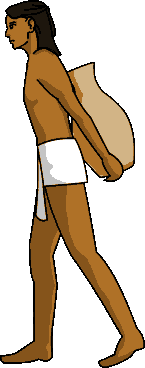
\includegraphics[scale=0.5]{Imagenes/hombre02}}
	\subfigure[Hombre con cacao.]{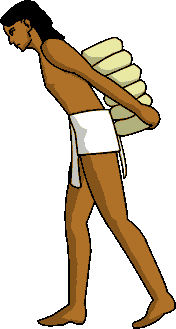
\includegraphics[scale=0.5]{Imagenes/hombre01}}
	\subfigure[Hombre noble.]{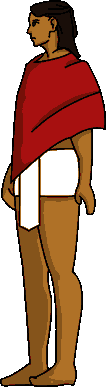
\includegraphics[scale=0.5]{Imagenes/hombre03}}
	\subfigure[Mujer con jarrón.]{
\includegraphics[scale=0.5]{Imagenes/mujer01}}
	\subfigure[Mujer de puesto.]{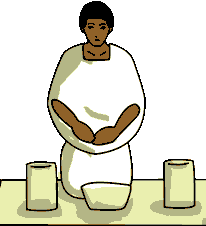
\includegraphics[scale=0.5]{Imagenes/mujer02}}
	\caption{Ciudadanos que se encuentran.}
	\label{fig:Ciudadanos}
\end{figure} 
\subsubsection{Concepto:}
Los ciudadanos se encuentran para relatar al jugador la época en la que se encuentra, la situación actual que enfrentan, el lugar donde se encuentran y más datos para entender el contexto que lo rodea.
\subsubsection{Encuentro:}
En el nivel 1.
\subsection{Nombre: Tunkuluchú}   \label{per.tecolote}
\subsubsection{Descripción:}
Ave de la familia de los buhos. En la mitología mexica este animal podía ingresar al inframundo y regresar al mundo sin restricciones. Este personaje se encuentra en todos los niveles con la función de un checkpoint.
\subsubsection{Status:}
NPC, checkpoint.
\subsubsection{Imagen}
Ver figura \ref{fig:tecolote}.
\begin{figure}
	\centering
	
\includegraphics[height=0.2 \textheight]{Imagenes/tecolote}
	\caption{Tecolote de nombre Tunkuluchú.}
	\label{fig:tecolote}
\end{figure}
\subsubsection{Encuentro:}
Todos los niveles.
\subsection{Nombre: Armadillo}  \label{per.armadillo} 
\subsubsection{Descripción:}
Animal de clima seco. Posee un caparazón dorsal formado por placas y con picos saliendo de estas, con cola bastante larga y extremidades cortas.
\subsubsection{Status:}
Enemigo
\subsubsection{Imagen}
Ver figura \ref{fig:armadillo}
\begin{figure}
	\centering
	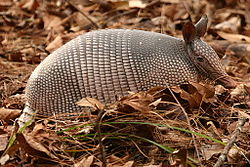
\includegraphics[height=0.2 \textheight]{Imagenes/armadillo}
	\caption{Armadillo.}
	\label{fig:armadillo}
\end{figure} 
\subsubsection{Concepto:}
Enemigo terrestre que se encarga de obstaculizar y dañar al jugador. Se encuentra por el suelo.
\subsubsection{Encuentro:}
Enemigo de la etapa tres del inframundo.
Nivel 4.
\subsubsection{Habilidades:}
\begin{itemize}
	\item Rodar. Ver habilidad \ref{hab.rodar}.
	\item Desenrrollarse. Ver habilidad \ref{hab.desenrrollar}.
\end{itemize}
\subsubsection{Patrón de ataque:}
En un ciclo, realizará la habilidad rodar tres veces y después la habilidad desenrrollarse una vez. Este ciclo se repetirá hasta que el enemigo desaparezca.

\subsection{Nombre: Fantasma rojo}   \label{per.fantasmaR}
\subsubsection{Descripción:}
Alma perdida en el Mictlán. Es un craneo flotate envuelto en una niebla roja.
Se enfrenta al jugador disparándole tonalli negativo para causarle daño. También si toca al jugador le hace daño. 
\subsubsection{Status:}
Enemigo.
\subsubsection{Imagen}
Ver figura \ref{fig:fantasmaR}.
\begin{figure}
	\centering
	
\includegraphics[height=0.2 \textheight]{Imagenes/fantasmaRojo}
	\caption{Fantasma rojo.}
	\label{fig:fantasmaR}
\end{figure} 
\subsubsection{Encuentro:}
Enemigo de los niveles 2, 3, 6, 7 y 9.
\subsubsection{Habilidades:}
\begin{itemize}
	\item Disparo rojo. Ver \ref{hab.disparoR}.
	\item Flotar en vertical. Ver \ref{hab.flotarV}.
\end{itemize}
\subsubsection{Patrón de ataque:}
En un ciclo, realizará la habilidad disparo rojo en todo momento mientras realiza la habilidad flotar en vertical. Este ciclo se repetirá hasta que el enemigo desaparezca.

\subsection{Nombre: Fantasma morado}   \label{per.fantasmaM}
\subsubsection{Descripción:}
Alma perdida en el Mictlán. Es un craneo flotate envuelto en una niebla morada.
Se enfrenta al jugador lanzándosele para causarle daño. Si toca al jugador le hace daño. 
\subsubsection{Status:}
Enemigo.
\subsubsection{Imagen}
Ver figura \ref{fig:fantasmaM}.
\begin{figure}
	\centering
	
\includegraphics[height=0.2 \textheight]{Imagenes/fantasmaMorado}
	\caption{Fantasma morado.}
	\label{fig:fantasmaM}
\end{figure}
\subsubsection{Encuentro:}
En niveles 2, 4, 5, 7, 9.
\subsubsection{Habilidades:}
\begin{itemize}
	\item Embestida. Ver habilidad \ref{hab.embestida}.
	\item Flotar en triángulo. Ver habilidad \ref{hab.flotarT}.
\end{itemize}
\subsubsection{Patrón de ataque:}
En un ciclo, realizará la habilidad embestida una vez y después la habilidad flotar en triángulo una vez. Este ciclo se repetirá hasta que el enemigo desaparezca.

\subsection{Nombre: Zopilote}   \label{per.zopilote}
\subsubsection{Descripción:}
Ave de rapiña, tiene un plumaje negro, su cabeza calva es de color gris oscuro y tiene un pico grisáceo.
\subsubsection{Status:}
Enemigo.
\subsubsection{Imagen}
Ver figura \ref{fig:zopilote}.
\begin{figure}
	\centering
	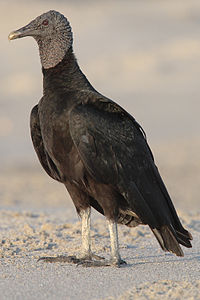
\includegraphics[height=0.2 \textheight]{Imagenes/zopilote}
	\caption{Zopilote.}
	\label{fig:zopilote}
\end{figure}
\subsubsection{Encuentro:}
En el nivel 5.
\subsubsection{Habilidades:}
\begin{itemize}
	\item Rapto. Ver habilidad en \ref{hab.rapto}.
	\item Zopilotear. Ver habilidad en \ref{hab.zopilotear}.
\end{itemize}
\subsubsection{Patrón de ataque:}
En un ciclo, realizará la habilidad rapto cuando se aproxime el jugador a una distancia determinada, mientras no se realice la habilidad rapto la habilidad zopilotear estará activada. Este ciclo se repetirá hasta que el enemigo desaparezca.
\subsection{Nombre: Jaguar}   \label{per.jaguar}
\subsubsection{Descripción:}
Animal felino carnívoro, de color amarillo a café rojizo con manchas negras.
\subsubsection{Status:}
NPC, enemigo.
\subsubsection{Imagen}
Ver figura \ref{fig:jaguar}.
\begin{figure}
	\centering
	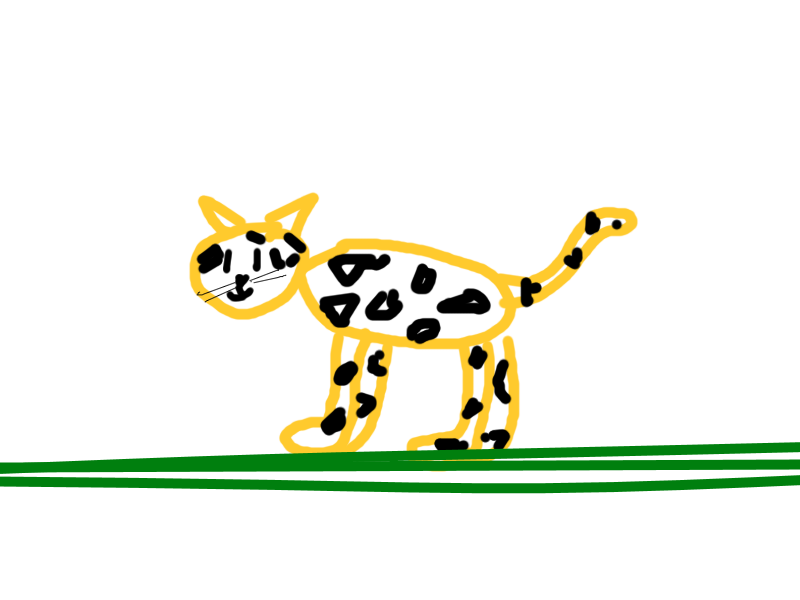
\includegraphics[height=0.2 \textheight]{Imagenes/jaguar}
	\caption{Jaguar.}
	\label{fig:jaguar}
\end{figure}
\subsubsection{Encuentro:}
En el nivel 8.
\subsubsection{Habilidades:}
\begin{itemize}
	\item Zarpazo. Ver en \ref{hab.zarpazo}.
\end{itemize}
\subsubsection{Patrón de ataque:}
El felino va de un lado hacia otro en dirección horizontal, cuando se encuentra con el jugador tira un zarpazo.

\section{Obstáculos}
	\subsection{Nombre: Caja} \label{obs.caja}
\subsubsection{Descripción}
Una caja de madera. El jugador al tocar tendrá una característica rígida. El jugador no podrá moverla, puede pararse sobre ella. No ocasiona ningún efecto adicional al tocarla.
\subsubsection{Esquema}
Ver figura \ref{fig:caja}.
\begin{figure}
	\centering
	
\includegraphics[height=0.2 \textheight]{Imagenes/caja}
	\caption{Caja de madera.}
	\label{fig:caja}
\end{figure}
	\subsection{Nombre: Sacos cacao}\label{obs.saco}
\subsubsection{Descripción}
Sacos de tela blanquezco. El jugador al tocar tendrá una característica rígida. El jugador no podrá moverla, puede pararse sobre ella. No ocasiona ningún efecto adicional al tocarla.
\subsubsection{Esquema}
Ver figura \ref{fig:saco}.
\begin{figure}
	\centering
	
\includegraphics[height=0.2 \textheight]{Imagenes/saco}
	\caption{Sacos de cacao.}
	\label{fig:saco}
\end{figure}
	\subsection{Nombre: Plataforma móvil}\label{obs.plataformaM}
	\subsubsection{Descripción}
	Pedazo de terreno (cualquiera) que está en constante movimiento siguiendo un mismo patrón. El jugador al contacto, la plataforma tiene una característica rígida, puede posarse sobre de él y seguir su trayectoria.
	\subsubsection{Esquema}
	Ver figura \ref{fig:plataformaM}.
	\begin{figure}
		\centering
		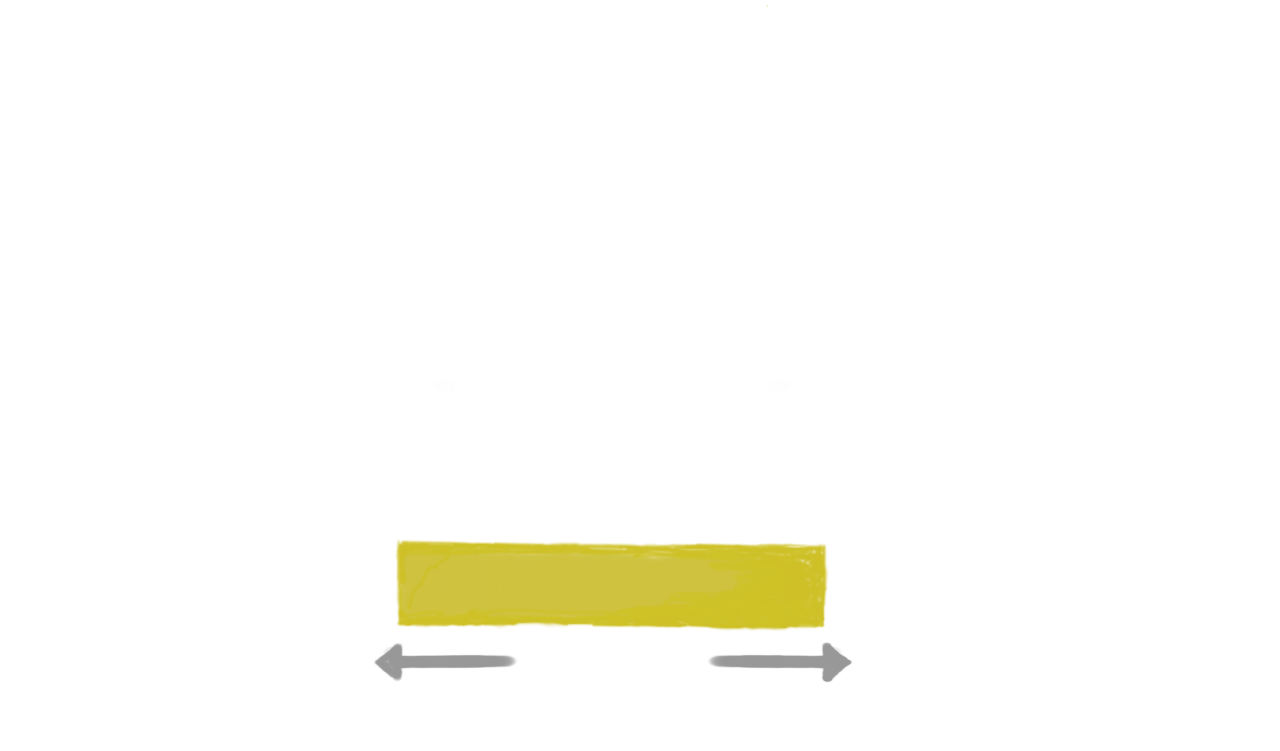
\includegraphics[height=0.2 \textheight]{Imagenes/plataformaM}
		\caption{Plataforma móvil.}
		\label{fig:plataformaM}
	\end{figure}
		\subsection{Nombre: Plataforma débil}\label{obs.plataformaD}
	\subsubsection{Descripción}
	Pedazo de terreno (cualquiera), de característica rígida. El jugador puede posarse sobre de esta, luego de pocos segundos la plataforma empieza a desaparecer. Luego de desaparecer, reaparece en segundos.
	\subsubsection{Esquema}
	Ver figura \ref{fig:plataformaD}.
	\begin{figure}
		\centering
		\includegraphics[height=0.2 \textheight]{Imagenes/plataformaD}
		\caption{Plataforma débil.}
		\label{fig:plafarmaD}
	\end{figure}
		\subsection{Nombre: Rocas}\label{obs.rocas}
	\subsubsection{Descripción}
	Conjunto de piedras o rocas posicionadas en un punto determinado, preferentemente alto. Este objeto cuenta con un área donde se detecta si ha pasado el jugador, de ser así las piedras caerán.
	\subsubsection{Esquema}
	Ver figura \ref{fig:rocas}.
	\begin{figure}
		\centering
		\includegraphics[height=0.2 \textheight]{Imagenes/rocas}
		\caption{Rocas cayendo cuando el jugador ha paso por el área.}
		\label{fig:rocas}
	\end{figure}
		\subsection{Nombre: Viento temporal}\label{obs.vientoT}
	\subsubsection{Descripción}
	Ráfaga de viento, este objeto no es rígido y puede ser visible solo por las animaciones ocasionales de líneas rectas horizontales pasando. El viento se activa por lapsos de tiempo constantes. El jugador al entrar en contacto con el viento le estará dando una velocidad constante negativa al eje horizontal, provocando un "empuje" del personaje. 
	\subsubsection{Esquema}
	Ver figura \ref{fig:vientoT}.
	\begin{figure}
		\centering
		\includegraphics[height=0.2 \textheight]{Imagenes/vientoT}
		\caption{Dirección que el viento toma respecto al jugador.}
		\label{fig:vientoT}
	\end{figure}
		\subsection{Nombre: Piedras filosas}\label{obs.piedrasF}
	\subsubsection{Descripción}
	Piedras puntiagudas en forma de triángulo. Sobresalen del piso o muro de un terreno, son rígidas y no poseen ningún movimiento. Al contacto con el jugador le restan puntos de vida.
	\subsubsection{Esquema}
	Ver figura \ref{fig:piedrasF}.
	\begin{figure}
		\centering
		\includegraphics[height=0.2 \textheight]{Imagenes/piedrasF}
		\caption{Sacos de cacao.}
		\label{fig:piedrasF}
	\end{figure}
		\subsection{Nombre: Piso congelado}\label{obs.pisoC}
	\subsubsection{Descripción}
	Pedazo de hielo congelado en el piso de un terreno, es rígido. Al contacto con el jugador quita toda fricción del piso, ocasionando que no exista suficiente control del jugador de su velocidad y dirección horizontal.
	\subsubsection{Esquema}
	Ver figura \ref{fig:pisoC}.
	\begin{figure}
		\centering
		\includegraphics[height=0.2 \textheight]{Imagenes/pisoC}
		\caption{Piso congelado.}
		\label{fig:pisoC}
	\end{figure}
		\subsection{Nombre: Hielo quebradizo}\label{obs.hieloQ}
	\subsubsection{Descripción}
	Pedazo de terreno, consta de hielo fracturado visualmente, es rígido. Al contacto con el jugador después de unos segundos empieza a desaparecer, reaparece luego de otros segundos más.
	\subsubsection{Esquema}
	Ver figura \ref{fig:hieloQ}.
	\begin{figure}
		\centering
		\includegraphics[height=0.2 \textheight]{Imagenes/hieloQ}
		\caption{Hielo quebradizo y como se rompe cuando el jugador se para en cima.}
		\label{fig:hieloQ}
	\end{figure}
		\subsection{Nombre: Bolas de nieve}\label{obs.bolasN}
	\subsubsection{Descripción}
	Conjunto de bolas de nieve, su característica es rígida. Posicionadas en un punto determinado, preferentemente alto. Este objeto cuenta con un área donde se detecta si ha pasado el jugador, de ser así las bolas de nieve caerán.
	\subsubsection{Esquema}
	Ver figura \ref{fig:bolasN}.
	\begin{figure}
		\centering
		\includegraphics[height=0.2 \textheight]{Imagenes/bolasN}
		\caption{Sacos de cacao.}
		\label{fig:bolasN}
	\end{figure}
		\subsection{Nombre: Viento multidireccional}\label{obs.vientoM}
	\subsubsection{Descripción}
		Ráfaga de viento, este objeto no es rígido y puede ser visible solo por las animaciones ocasionales de líneas rectas (horizontales, verticales, diagonales). El viento se activa por lapsos de tiempo constantes. El jugador al entrar en contacto con el viento le estará dando una velocidad constante en una dirección aleatoria que podría ser horizontal, vertical o en diagonal, provocando un "empuje" del personaje. 
	\subsubsection{Esquema}
	Ver figura \ref{fig:vientoM}.
	\begin{figure}
		\centering
		\includegraphics[height=0.2 \textheight]{Imagenes/vientoM}
		\caption{Sacos de cacao.}
		\label{fig:vientoM}
	\end{figure}
		\subsection{Nombre: Lluvia de flechas}\label{obs.lluviaF}
	\subsubsection{Descripción}
	Consiste en flechas cayendo aleatoriamente sobre el eje horizontal hacia el piso y constantemente. Al contacto con el jugador le resta puntos de vida.
	\subsubsection{Esquema}
	Ver figura \ref{fig:lluviaF}.
	\begin{figure}
		\centering
		\includegraphics[height=0.2 \textheight]{Imagenes/lluviaF}
		\caption{Lluvia de flechas representada en un nivel.}
		\label{fig:lluviaF}
	\end{figure}

\section{Habilidades.}
	\subsection{Nombre: Rodar.} \label{hab.rodar}
		\subsubsection{Descripción}
		El enemigo en forma circular se desplazará rodando a lo largo del suelo en dirección horizontal.
		Rodará hasta llegar al extremo de una plataforma o al proximarse a un muro.
		\subsubsection{Portador}
		Armadillo. Ver \ref{per.armadillo}.
		\subsubsection{Esquema}
		Ver figura \ref{fig:rodar}.
		\begin{figure}
			\centering
			\includegraphics[height=0.2 \textheight]{Imagenes/rodar}
			\caption{Rodar.}
			\label{fig:rodar}
		\end{figure}
	\subsection{Nombre: Desenrrollar.} \label{hab.desenrrollar}
		\subsubsection{Descripción}
		El enemigo pasará a un estado estático. El enemigo visualmente cambiará de forma circular a su forma natural.
		\subsubsection{Portador}
		Armadillo. Ver \ref{per.armadillo}.
		\subsubsection{Esquema}
		Ver figura \ref{fig:desenrrollar}.
		\begin{figure}
			\centering
			\includegraphics[height=0.2 \textheight]{Imagenes/desenrrollar}
			\caption{Desenrrollar.}
			\label{fig:desenrrollar}
		\end{figure}
	\subsection{Nombre: Disparo rojo.} \label{hab.disparoR}
		\subsubsection{Descripción}
		El enemigo lanza pequeños círculos rojos en dirección horizontal que dañan al jugador. Los disparos salen de la parte frontal del enemigo.
		\subsubsection{Portador}
		Fantasma rojo. Ver \ref{per.fantasmaR}.
		\subsubsection{Esquema}
		Ver figura \ref{fig:disparoR}.
		\begin{figure}
			\centering
			\includegraphics[height=0.2 \textheight]{Imagenes/disparoR}
			\caption{Disparo rojo.}
			\label{fig:disparoR}
		\end{figure}
	\subsection{Nombre: Flotar en vertical.} \label{hab.flotarV}
		\subsubsection{Descripción}
		El enemigo se desplaza sobre el piso, moviéndose de manera vertical. Llega a determinada altura y vuelve a bajar al piso.
		\subsubsection{Portador}
		Fantasma rojo. Ver \ref{per.fantasmaR}.
		\subsubsection{Esquema}
		Ver figura \ref{fig:flotarV}.
		\begin{figure}
			\centering
			\includegraphics[height=0.2 \textheight]{Imagenes/flotarV}
			\caption{Flotar en vertical.}
			\label{fig:flotarV}
		\end{figure}
	\subsection{Nombre: Embestida.} \label{hab.embestida}
		\subsubsection{Descripción}
		El enemigo aumenta su velocidad mientras se desplaza de arriba hacia abajo en diagonal.
		\subsubsection{Portador}
		Fantasma morado. Ver \ref{per.fantasmaM}.
		\subsubsection{Esquema}
		Ver figura \ref{fig:embestida}.
		\begin{figure}
			\centering
			\includegraphics[height=0.2 \textheight]{Imagenes/embestida}
			\caption{Embestida.}
			\label{fig:embestida}
		\end{figure}
	\subsection{Nombre: Flotar en triángulo.} \label{hab.flotarT}
		\subsubsection{Descripción}
		El enemigo se mueve por tres diferentes nodos, dibujando un triángulo. Al final regresa al primer nodo.
		\subsubsection{Portador}
		Fantasma morado. Ver \ref{per.fantasmaM}.
		\subsubsection{Esquema}
		Ver figura \ref{fig:flotarT}.
		\begin{figure}
			\centering
			\includegraphics[height=0.2 \textheight]{Imagenes/flotarT}
			\caption{Flotar en triángulo.}
			\label{fig:flotarT}
		\end{figure}
	\subsection{Nombre: Rapto.} \label{hab.rapto}
		\subsubsection{Descripción}
		El enemigo se mueve hacia la posición del jugador, lanzándose de su posición hacia abajo con una desviación curva.
		\subsubsection{Portador}
		Zopilote. Ver \ref{per.zopilote}.
		\subsubsection{Esquema}
		Ver figura \ref{fig:rapto}.
		\begin{figure}
			\centering
			\includegraphics[height=0.2 \textheight]{Imagenes/rapto}
			\caption{Zopilote.}
			\label{fig:rapto}
		\end{figure}
	\subsection{Nombre: Zopilotear.} \label{hab.zopilotear}
		\subsubsection{Descripción}
		El enemigo se mueve de manera circular por sobre el piso.
		\subsubsection{Portador}
		Zopilote. Ver \ref{per.zopilote}.
		\subsubsection{Esquema}
		Ver figura \ref{fig:zopilotear}.
		\begin{figure}
			\centering
			\includegraphics[height=0.2 \textheight]{Imagenes/zopilotear}
			\caption{Zopilotear.}
			\label{fig:zopilotear}
		\end{figure}
			\subsection{Nombre: Zarpazo.} \label{hab.zarpazo}
			\subsubsection{Descripción}
			El enemigo con sus garras ataca al jugador.
			\subsubsection{Portador}
			Jaguar. Ver \ref{per.jaguar}.
			\subsubsection{Esquema}
			Ver figura \ref{fig:zarpazo}.
			\begin{figure}
				\centering
				\includegraphics[height=0.2 \textheight]{Imagenes/zarpazo}
				\caption{Zarpazo.}
				\label{fig:zarpazo}
			\end{figure}
\subsection{Nombre: Disparo de tonalli.}\ref{hab.disparoT}
\subsubsection{Descripción}
Con ayuda de la caracola permite a su portador disparar tonalli.
\subsubsection{Portador}
Malinalli
\subsubsection{Esquema}
			Ver figura \ref{fig:disparoT}.
			\begin{figure}
				\centering
				\includegraphics[height=0.2 \textheight]{Imagenes/disparoT}
				\caption{Disparo de tonalli por el jugador.}
				\label{fig:disparoT}
			\end{figure}
\subsection{Nombre: Zambullida.}\ref{hab.zambullida}
\subsubsection{Descripción}
Zochitónal se sumerge en el río, dejando solo en la superficie parte de su espalda; procediendo a nadar a gran velocidad de un lado a otro para embestir a sus enemigos.  
\subsubsection{Portador}
Zochitónal
\subsubsection{Esquema}
			Ver figura \ref{fig:zambullida}.
			\begin{figure}
				\centering
				\includegraphics[height=0.2 \textheight]{Imagenes/zambullida}
				\caption{Zambullida.}
				\label{fig:zambullida}
			\end{figure}
\subsection{Nombre: Burbujas.}
\subsubsection{Descripción}
Zochitónal dispara burbujas que seguirán al jugador por un tiempo.  
\subsubsection{Portador}
Zochitónal
\subsubsection{Esquema}
			Ver figura \ref{fig:burbujas}.
			\begin{figure}
				\centering
				\includegraphics[height=0.2 \textheight]{Imagenes/burbujas}
				\caption{Burbujas.}
				\label{fig:burbujas}
			\end{figure}
\subsection{Nombre: Coraza.}
\subsubsection{Descripción}
Esta habilidad permite crear una coraza de piedra protegiendo a su portador de ataques enemigos sacrificando velocidad de movimiento.  
\subsubsection{Portador}
Tepeyóllotl.
\subsubsection{Esquema}
			Ver figura \ref{fig:coraza}.
			\begin{figure}
				\centering
				\includegraphics[height=0.2 \textheight]{Imagenes/coraza}
				\caption{Coraza.}
				\label{fig:coraza}
			\end{figure}
\subsection{Nombre: Impacto.}
\subsubsection{Descripción}
Realiza un salto, provocando al aterrizaje una onda de piedras en el suelo.
\subsubsection{Portador}
Tepeyóllotl.
\subsubsection{Esquema}
\subsection{Nombre de la habilidad: Luvia de rocas.}
\subsubsection{Descripción}
Con un poderoso rugido provoca una avalancha de rocas. 
\subsubsection{Portador}
Tepeyóllotl.
\subsubsection{Esquema}
			Ver figura \ref{fig:lluviaR}.
			\begin{figure}
				\centering
				\includegraphics[height=0.2 \textheight]{Imagenes/lluviaR}
				\caption{Lluvia de rocas.}
				\label{fig:lluviaR}
			\end{figure}
\subsection{Nombre: Rugido aturdidor.}
\subsubsection{Descripción}
Poderoso rugido provoca una de continuo echo que inmoviliza a al enemigo, Tepeyóllotl solo puede usar esta habilidad cuando no usa la coraza. 
\subsubsection{Portador}
Tepeyóllotl. 
\subsubsection{Esquema}
			Ver figura \ref{fig:rugido}.
			\begin{figure}
				\centering
				\includegraphics[height=0.2 \textheight]{Imagenes/rugido}
				\caption{Rugido aturdidor.}
				\label{fig:rugido}
			\end{figure}
\subsection{Nombre: Circulo de fuego.}
\subsubsection{Descripción}
Itzpápalotl se eleva en el aire y se rodea a sí misma con fuego, este ataque sera usado cuando el jugador se encuentre junto a ella.
\subsubsection{Portador}
Itzpápalotl. 
\subsubsection{Esquema}
			Ver figura \ref{fig:circuloF}.
			\begin{figure}
				\centering
				\includegraphics[height=0.2 \textheight]{Imagenes/circuloF}
				\caption{Círculo de fuego.}
				\label{fig:circuloF}
			\end{figure}
\subsection{Nombre: Embestida aerea.}
\subsubsection{Descripción}
Itzpápalotl usara este ataque cuando este lejos del jugador. Itzpápalotl saltar y en el aire se lanza contra el enemigo en diagonal.
\subsubsection{Portador}
Itzpápalotl.
\subsubsection{Esquema}
			Ver figura \ref{fig:embestidaA}.
			\begin{figure}
				\centering
				\includegraphics[height=0.2 \textheight]{Imagenes/embestidaA}
				\caption{Embestida aerea.}
				\label{fig:embestidaA}
			\end{figure}
\subsection{Nombre: Invisibilidad.}
\subsubsection{Descripción}
Esta habilidad le permite ser indetectable al ojo de dioses y humanos, permitiendole tomar una posición ventajosa en combate.
\subsubsection{Portador}
Itzpápalotl.
\subsubsection{Esquema}
			Ver figura \ref{fig:invisibilidad}.
			\begin{figure}
				\centering
				\includegraphics[height=0.2 \textheight]{Imagenes/invisibilidad}
				\caption{Invisibilidad.}
				\label{fig:invisibilidad}
			\end{figure}
\subsection{Nombre: Tornado.}
\subsubsection{Descripción}
Poderoso ataque que puede bajar hasta la mitad de la vida del jugador.
\subsubsection{Portador}
Mictlecayotl.
\subsubsection{Esquema}
			Ver figura \ref{fig:tornado}.
			\begin{figure}
				\centering
				\includegraphics[height=0.2 \textheight]{Imagenes/tornado}
				\caption{Tornado.}
				\label{fig:tornado}
			\end{figure}
\subsection{Nombre: Ventisca.}
\subsubsection{Descripción}
Aire helado que puede causar una pérdida considerable de la barra de salud.
\subsubsection{Portador}
Mictlecayotl.
\subsubsection{Esquema}
			Ver figura \ref{fig:ventisca}.
			\begin{figure}
				\centering
				\includegraphics[height=0.2 \textheight]{Imagenes/ventisca}
				\caption{Ventisca.}
				\label{fig:ventisca}
			\end{figure}
\subsection{Nombre: Raíz del diablo.}
\subsubsection{Descripción}
Ataque que produce una confusión en el jugador, haciendo que los botones no reaccionen con las acciones que deberían.
\subsubsection{Portador}
Tlazoltéotl.
\subsubsection{Esquema}
			Ver figura \ref{fig:raiz}.
			\begin{figure}
				\centering
				\includegraphics[height=0.2 \textheight]{Imagenes/raiz}
				\caption{Raíz del diablo.}
				\label{fig:raiz}
			\end{figure}
\subsection{Nombre: Energía corrupta.}
\subsubsection{Descripción}
Esferas de energia oscura que infringen daño al jugador al hacer contacto con éste.
\subsubsection{Portador}
Tlazoltéotl.
\subsubsection{Esquema}
			Ver figura \ref{fig:energiaC}.
			\begin{figure}
				\centering
				\includegraphics[height=0.2 \textheight]{Imagenes/energiaC}
				\caption{Energía corrupta.}
				\label{fig:energiaC}
			\end{figure}	
\subsection{Nombre: Circulo protector.}
\subsubsection{Descripción}
Utilizando energía corrupta,  Tlazoltéotl crea alrededor de ella un circulo con la capacidad de protegerla contra cualquier ataque.
\subsubsection{Portador}
Tlazoltéotl.
\subsubsection{Esquema}
			Ver figura \ref{fig:circuloP}.
			\begin{figure}
				\centering
				\includegraphics[height=0.2 \textheight]{Imagenes/circuloP}
				\caption{Círculo protector.}
				\label{fig:circuloP}
			\end{figure}
\subsection{Nombre: LLuvia de lava.}
\subsubsection{Descripción}
Caen bolas de lava con una gran capacidad de daño.
\subsubsection{Portador}
Itztlacoliuhqui.	
\subsubsection{Esquema}	
			Ver figura \ref{fig:lluviaL}.
			\begin{figure}
				\centering
				\includegraphics[height=0.2 \textheight]{Imagenes/lluviaL}
				\caption{Lluvia de lava.}
				\label{fig:lluviaL}
			\end{figure}
\subsection{Nombre: Manotazo.}
\subsubsection{Descripción}
Genera una onda expansiva que deforma el suelo provonado una oleada de rocas.
\subsubsection{Portador}
\subsubsection{Esquema}
			Ver figura \ref{fig:manotazo}.
			\begin{figure}
				\centering
				\includegraphics[height=0.2 \textheight]{Imagenes/manotazo}
				\caption{Manotazo.}
				\label{fig:manotazo}
			\end{figure}
Itztlacoliuhqui.
\subsection{Nombre: Lluvia de flechas.}
\subsubsection{Descripción}
Como su nombre lo dice, provoca una lluvia de flechas, este es el ataque de Itztlacoliuhqui que genera el menor nivel de daño. 
\subsubsection{Portador}
Itztlacoliuhqui.
\subsubsection{Esquema}
			Ver figura \ref{fig:lluviaF}.
\subsection{Nombre: Todos los hombres del rey.}
\subsubsection{Descripción}
Con este ataque,  Mictlantechtli invoca a varios de los enemigos normales que habitan el Mictlán para que se enfrenten al jugador mientras  Mictlantechhtli desaparece.
\subsubsection{Portador}
Mictlantechtli.
\subsubsection{Esquema}
			Ver figura \ref{fig:rey}.
			\begin{figure}
				\centering
				\includegraphics[height=0.2 \textheight]{Imagenes/rey}
				\caption{Todos los hombres del rey.}
				\label{fig:rey}
			\end{figure}
\subsection{Nombre: Fuego mortífero.}
\subsubsection{Descripción}
Mictlantechtli  lanza poderosas esferas de fuego verde.
\subsubsection{Portador}
Mictlantechtli.	
\subsubsection{Esquema}	
			Ver figura \ref{fig:fuegoM}.
			\begin{figure}
				\centering
				\includegraphics[height=0.2 \textheight]{Imagenes/fuegoM}
				\caption{fuegoM.}
				\label{fig:fuegoM}
			\end{figure}
\subsection{Nombre: Penitencia.}
\subsubsection{Descripción}
Mictlantechtli se eleva en el aire haciendo que salgan huesos filosos del suelo.
\subsubsection{Portador}
Mictlantechtli.
\subsubsection{Esquema}
			Ver figura \ref{fig:penitencia}.
			\begin{figure}
				\centering
				\includegraphics[height=0.2 \textheight]{Imagenes/penitencia}
				\caption{Penitencia.}
				\label{fig:penitencia}
			\end{figure}


\section{Armas.}
\subsection{Nombre: Caracola.}
\subsubsection{Descripción}
Esta arma con forma de cenzontle contiene el alma de uno dentro, lo que le permita generar todo tipo de sonidos. El sonido que produce se ve materializado como energía luminosa que puede atacar a los enemigos y proteger a su portador al generar una barrera.
\subsubsection{Imagen}
\subsubsection{Portador}
Malinalli.

\subsection{Nombre: Atardecer de venus.}
\subsubsection{Descripción}
áculo que permite amplificar la magia de quien lo porta. Xólotl solamente puede utilizarlo en su forma humana.
\subsubsection{Imagen}
\subsubsection{Portador}
Xólotl.

\subsection{Nombre: Matlalpapalotl.}
\subsubsection{Descripción}
Tepoztopilli hecho de obsidiana. Arma creada por Iztpapalotl a partir de las almas de los enemigos derrotados durante la guerra contra los dioses del norte. Es un arma de gran poder, es ligera, ideal para el combate aéreo.
\subsubsection{Imagen}
\subsubsection{Portador}
Itzpápalotl.

\subsection{Nombre: Trepa viento.}
\subsubsection{Descripción}
Macuahuitl creada por Mictlecayotl para canalizar su energía de viento y generar poderoso ataques.
\subsubsection{Imagen}
\subsubsection{Portador}
Macuahuitl.

\subsection{Nombre: Arco solar.}
\subsubsection{Descripción}
Arma legendaria que Itztlacoliuhqui usaba desde antes del quinto Sol, siendo éste el único objeto que se le permiti conservar de su antigua identidad. Es un arco de gran alcance, permite disparar flechas con la capacidad de destruir mundos enteros. 
\subsubsection{Imagen}
\subsubsection{Portador}
Itztlacoliuhqui.



\section{Items.}
	\subsection{Nombre: Peineta en forma de flor.}
	\subsubsection{Descripción}
	Fue un regalo de su padre cuando niña, Malinalli la considera su mayor tesoro.
	\subsubsection{Imagen}
	\subsubsection{Portador}
	Malinalli 

	\subsection{Nombre: Armadura espiritual.}
	\subsubsection{Descripción}
	Cubre todo el cuerpo de Malinalli, pero visualmente adopta una forma que ella desee.
	\subsubsection{Imagen}
	\subsubsection{Portador}
	Malinalli 

\section{Guión.}

\section{Música  y sonidos.}
\subsection{Música  de fondo}
\subsubsection{Nombre: Música  mercado}
La música de fondo que suena en el mercado debe de evocar un sentimiento de cotidianidad, seguridad y alegría. En el tema predominaran instrumentos de viento. 		
\subsubsection{Nombre: Música  selva}
La música en la selva debe de ser sobre inicio de un viaje. Debe de evocar en el jugador el deseo de aventura y a la vez hacerlo sentir que está en un lugar conocido.
\subsubsection{Nombre: Música  Xolotl} 
La música cuando Xólotl le habla a Malinalli debe de ser un tema que se ajuste con la personalidad del Dios ya que será el tema que sonara cuando él tenga diálogos importantes que decir, así que debe ser un tema que muestre determinación y misterio.
\subsubsection{Nombre: Música plataforma segundo nivel}
La musicalización que corresponde a la zona de enemigos normales de este nivel debe de reflejar que uno se encuentra en la entrada de un lugar misterios y peligroso, pero de gran carga espiritual (Por lo que se recomienda alguna canción que contenga coros, los coros preferiblemente deben de estar en Náhualt y deben de hablar sobre el sufrimiento de las almas que no pudieron cruzar).
\subsubsection{Nombre: Música jefe segundo nivel}
La música que acompaña a la batalla con Xochitonal debe de hacer sentir peligro que se está luchando por sobrevivir pero sin perder la carga espiritual que conlleva este nivel. 
\subsubsection{Nombre: Música plataforma tercer nivel} Zona de plataformas: La Música  de este nivel debe reflejar el sentimiento de adrenalina y vértigo que lleva escalar una superficie frágil y peligrosa.
\subsubsection{Nombre: Música jefe tercer nivel} 
Batalla contra el jefe: La batalla contra el jefe debe de mostrar un tema que evoque la misma adrenalina de peligro con el agregado de que la sensación de peligro se intensifica.

\subsubsection{Nombre: Música plataforma cuarto nivel}
La música del nivel evoca a que se está explorando un lugar misterioso y peligroso pero lleno de maravillas.
\subsubsection{Nombre: Música jefe cuarto nivel} 
La música de batalla contra el jefe debe de reflejar el ritmo desenfrenado de batalla que tiene Itzpapálotl, se propone una canción parecida a Bipolar Nightmare de la banda sonora de Nier Automata.

\subsubsection{Nombre: Música plataforma quinto nivel}
Este tema se caracterizara por tener una fuerte carga de nostalgia y renuncia hacia las personas que se aman, ya que representa la nostalgia que siente Mictlecayotl por todo lo que perdió cuando fue condenada a estar en el Mictlán por tratar de asesinar a Tezcatlipoca. El tema puede contener algunas notas como de caja de música y coros.
\subsubsection{Nombre: Música jefe quinto nivel} 
Este tema debe de contener un poco de la nostalgia pero a su vez debe de denotar fuerza y violencia. Su ritmo debe de ser acelerado pues refleja la personalidad de fuerte e innegociable de Mictlecayotl.


\subsubsection{Nombre: Música plataforma sexto nivel}
\subsubsection{Nombre: Música jefe sexto nivel} 


\subsection{Efectos de sonido}

\section{Imagenes de concepto.}
	\begin{figure}
	\centering
	\includegraphics[height=0.4 \linewidth]{Imagenes/Itztlacoliuhqui02}
	\caption{Itztlacoliuhqui.}
	\label{fig:itztla02}
	\end{figure}
	\begin{figure}
	\centering
	\includegraphics[height=0.4 \linewidth]{Imagenes/MalinalliBatalla}
	\caption{Malinalli.}
	\label{fig:malliB}
\end{figure}
	\begin{figure}
	\centering
	\includegraphics[height=0.4 \linewidth]{Imagenes/MalinalliConcepto}
	\caption{Malinalli.}
	\label{fig:bMalinalli}
\end{figure}
	\begin{figure}
	\centering
	\includegraphics[height=0.4 \linewidth]{Imagenes/MalinalliEsclava}
	\caption{Malinalli.}
	\label{fig:malliE}
\end{figure}
	\begin{figure}
	\centering
	\includegraphics[height=0.4 \linewidth]{Imagenes/MalinalliSprite}
	\caption{Malinalli sprite.}
	\label{fig:malliS}
\end{figure}

\begin{figure}
\centering
\includegraphics[height=0.4 \linewidth]{Imagenes/XolotlSprite}
\caption{Sprite de Xolotl.}
\label{fig:xoloS}
\end{figure}

\section{Miembros de equipo.}

\section{Detalles de producción.}
\subsection{Fecha de inicio.}
\subsection{Fecha de terminación.}
\subsection{Presupuesto.}

\printglossary
\end{document}